% \documentclass{cumcmthesis}
\documentclass[withoutpreface,bwprint]{cumcmthesis} %去掉封面与编号页
    \title{基于贪心算法的多波束测深测线最优布设方案设计}
    \tihao{B}            % 题号
    \baominghao{202319060034}    % 报名号
    \schoolname{哈尔滨工业大学(深圳)}
    \membera{刘沛权}
    \memberb{周锐皆}
    \memberc{陈佳锐}
    \supervisor{陈勇勇}
    \yearinput{2023}     % 年
    \monthinput{9}      % 月
    \dayinput{10}        % 日

    \begin{document}
        \maketitle
        \begin{abstract}
            使用搭载多波束系统的测量船沿一定路线获取海底深度数据是目前海底测深的主流方案。其中,测线的布设方案对测量的效率与数据质量
            有显著影响。
            本文基于\textbf{几何分析方法与贪心算法}给出了理想海底面下的测线最优布设方案,得出一般性结论并从理论角度证明该方案的最优性。
            最后,根据理想最优布设方案,通过数值模拟,给出了一个真实非理想海底面下的较优布设方案。

        \textbf{针对问题一},本文将平坦海底上的覆盖宽度和重叠率的基本定义扩展到非平坦海底情形,然后将覆盖宽度与重叠部分宽度的求解转化为平面几何问题,并利用\textbf{波束的
        对称性}与\textbf{角平分线的性质}简化覆盖宽度的计算,并给出任意深度下覆盖宽度 $W$ 与重叠率 $\eta$ 的关系:$ \eta = 1 - \frac{\cos\alpha\cos\frac{\theta}{2}}{\cos(\alpha - \frac{\theta}{2})}\frac{d}{W}$。
        根据上式,
        可得到不同离中心点不同距离的测线的覆盖宽度与重叠率,结果详细见 \cref{table:1}。

        \textbf{针对问题二},本文利用\textbf{矢量分解}方法,给出了不同方向测线的爬升率与海底深度分布。选取垂直于测线的视角,将三维空间中的问题简化
        为平面解三角形问题,并通过计算爬升率确定三角形形状,再次利用波束的对称性与角平分线的性质,求得覆盖宽度 $W$ 与海底深度 $D$、测线方向 $\beta$的关系:
        $W = D\sin\frac{\theta}{2}(\frac{1}{\cos(\frac{\theta}{2}+\gamma)} + \frac{1}{\cos(\frac{\theta}{2} - \gamma)})\cos\gamma$,其中 $\gamma = \arctan(\sin\beta\tan\alpha)$,
        最终给出不同方向测线上离中心点不同距离处的覆盖宽度,结果详细见 \cref{table:2}。
        
        \textbf{针对问题三},本文仅考虑测线间相互平行的情况,用测线角度与测线起始点来描述布线方案。本文先验证了沿坡度方向布线必然无法满足重叠率要求,基于两种重叠率定义,
        给出了满足重叠率要求的 $\beta$ 可行角度范围:$90^\circ\sim 91.026^\circ$或$90^\circ\sim 91.824^\circ$。接下来,本文使用\textbf{贪心算法},根据波束
        路径的可逆性提出了一种根据当前测线起始点计算下一条最优测线起始点的算法,从而可以计算给定测线角度下的一组最优起始点。本文在可行角度范围内进行搜索,得出最短测线长度为
        $125936.0$m,对应角度$ \beta = 90.0^\circ$,即测线与等深线平行的情形。更进一步地,本文证明了一个\textbf{通用结论}:在坡度恒定的理想海底上,沿等深线方向设置测线总是最优的。
        
        \textbf{针对问题四},本文先将原题多目标优化问题转化为以最小化测线总长度为目标,以漏测率,重叠率在合理范围内为约束的单目标约束优化问题。先通过边界条件确定了一条初始最优测线,在给定端点重叠率下,使用\textbf{贪心算法}不断确定下一条最优测线,直到覆盖海域边界。
        为使测线排布方案适应不同海域地形特征,本文在此基础上又提出了两种优化方案:1. 基于当前测线的相关指标动态调整下一条测线的端点重叠率。 2. 将海域划分为多个区域,在每个区域采用不同端点重叠率
        计算。经比较,得出测线最优布设方案及指标如下:\textbf{测线的总长度}:$407050$m,\textbf{漏测海区占总待测海域面积的百分比}:$4.73\%$,\textbf{重叠率超过$20\%$的总长度}:$40600$m。



            \keywords{多波束测深\quad  贪心算法\quad  数值模拟\quad}
        \end{abstract}
        % \tableofcontents % 目录
        \section{问题重述}
        \subsection{问题背景}
        海底地貌建模是海底地理研究的一个重要方向与手段,而海底深度测量是海底地貌建模的一个核心步骤。在现代海底深度测量工作中,一般使用测量船按既定航线
        获取深度数据。具体的深度数据获取方式又分为单波束测量和多波束测量。其中,单波束测量会导致测线之间完全没有数据,必须采用更小的测线间距(意味着更长的总
        测线长度与更大的航行成本)来保证数据不过分稀疏。为提高测量效率,一般使用多波束测量来获取更为稠密与鲁棒的数据。已知重叠率过小时可能发生漏测,即部分较
        浅的海底没有被测量,重叠率过大时会造成总测线长度的快速上升,进而导致资源的浪费。因此,如何针对不同海域地形特性,规划合理的测线图(包括测线方向与间距),
        使其在漏测率、重叠率、总测线距离上均有良好表现,是一个值得研究的重要问题。

        \subsection{问题重述}

        \textbf{问题一}:假设海底仍在测线方向上深度保持不变,但在垂直测线的面内有一定坡度,深度均匀变化,完成以下三个任务:
            $1$.给定坡度$\alpha$与当前位置(中心点)的海底深度 $D_0$,求出测线上各个位置对应的海底深度 $D$ 。
            $2$.基于几何关系建立多波束覆盖宽度$W$到重叠率$\eta$的函数关系。
            $3$.根据$1$中求出海底深度 $D$,基于几何关系计算测线上各个位置的覆盖宽度 $W$,并在给定波束张角等参数下用$2$中建立的模型求解测线上各个位置的重叠率 $\eta$。

        \textbf{问题二}:假设海底仍为有坡度的平面,测线与海底法向量、水平面法向量张成的平面形成了一个角度$\pi - \beta$,可将原问题分解为两个子问题:
            $1$. 给定坡度$\alpha$、测线角$\beta$以及当前位置(中心点)的海底深度 $D_0$,求出测线上各个位置对应的海底深度 $D$。
            $2$. 根据$1$中求出的海底深度 $D$,基于几何关系计算测线上各个位置的覆盖宽度 $W$。
        
        \textbf{问题三}:假设海底仍为有坡度的平面,给定一个矩形的海域范围,要求给出最优的测线排布方案,使得总测线距离最短,同时满足以下约束:
               $1$. 测线上各个位置与相邻测线的重叠率 $\eta$ 在$10\%\sim 20\%$之间。
               $2$. 测量范围覆盖全海底,即无漏测部分。

        \textbf{问题四}:给定海底深度的单波束测量数据,据此分析海底的地形特征与地形分布,并给出最优的测线排布方案,使得:
        $1$.总测线距离尽可能短。
        $2$.测量覆盖率尽可能大。
        $3$.重叠率尽量控制在 $20\%$ 以内。

        \section{问题分析}
        \subsection{问题一的分析}
        问题一需要求解斜面上的重叠率计算公式,以此计算不同深度下的重叠率。
        根据题目中给出的水平面上重叠率的计算公式进行类比,可将测线在斜面上的覆盖宽度投影在水平面上进行计算,通过投影长度给出斜面上重叠率的计算公式。
        然后,通过船只所处位置计算该点水深,带入公式得到重叠率,以此求出船只在不同位置的水深及重叠率。
        
        
        
        \subsection{问题二的分析}
        问题二需要考虑的是一个矩形海域,需要求解的是
        测线覆盖宽度与测量船距海域中心点距离及在测线方向与坡面方向在水平平面的投影的夹角 $\beta$ 的关系。
        首先根据坡面夹角 $\alpha$ 与船距中心点距离以及 测线角$\beta$ 可以求解出测线上各个位置的海底深度 $D$,
        然后计算出海底爬升率 $\varphi$ 的值,
        并根据问题一建立的水深与覆盖宽度的关系,求出测线上各个位置对应的覆盖宽度 $W$。
        \subsection{问题三的分析}
        问题三要求解出约束条件下的最短总测线距离,是一个约束优化问题,故需要先解决两个先置问题:如何将测线排布方案参数化与如何简化约束。
        
        首先要确定测线的形状,由于航船转弯时船头方向与运动方向不完全一致\cite{bib_1},而船头方向为波束面法向量,即无法从确定的航线中得到
        确定的波束覆盖范围,且船体转弯带来的摇晃对测量也会产生影响,故本文不考虑航船的测线为曲线的情况,以下讨论默认所有测线均为直线。

        接下来考虑不同测线之间是否平行的问题。一般的测线布置原则为沿等深线方向尽可能平行排布\cite{bib_2},故本文主要考虑测线之间互相平行
        的情况,并将在问题三的模型建立部分具体比较非平行测线与平行测线的情况。

        综上,每种测线方案可以用测线与坡度方向的夹角、相邻测线间的测线间距唯一表示。

        测线方案必须满足相邻条带重叠率在$10\%\sim 20\%$,并保证无漏测部分。相邻条带的重叠率一般指相邻条带中重叠部分的面积与条带面积之比,本文称
        该定义下的重叠率为全面积重叠率,记为$\eta_S$。
        
        重叠率的主要考量在于多波束系统中边缘波束精度低于中心波束,故需要保证相邻条带有一定重叠部分,来尽可能减小边缘部分的误差\cite{bib_3}。
        由此可知,比起相邻条带重叠面积的大小,条带边缘部分是否总能被两个波束覆盖更为重要。\cref{fig:accuracy}给出了一个全面积重叠率较高但并未保证边缘部分的低精度区被
        多个波束覆盖、甚至发生漏测的例子。
        \begin{figure}[H]
            \centering
            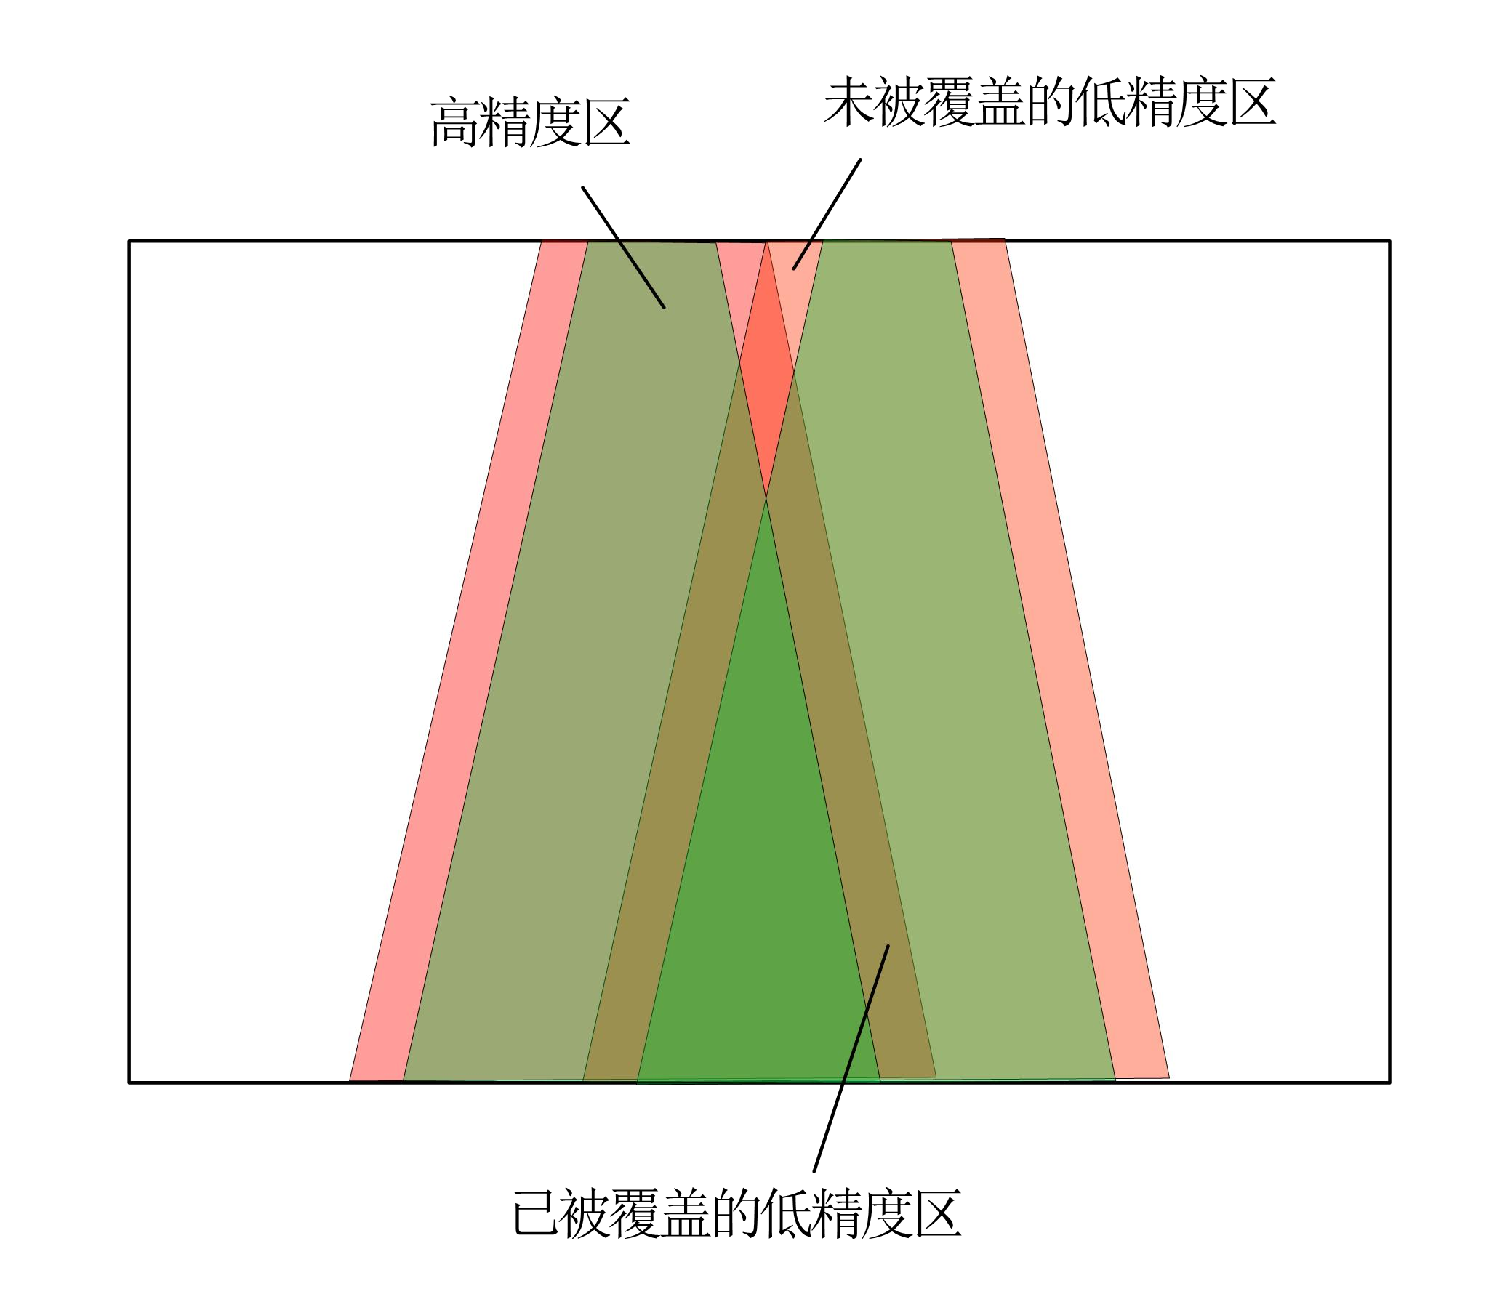
\includegraphics[width=.8\textwidth]{accuracy}
            \caption{一个全面积重叠率失效的实例}
            \label{fig:accuracy}
        \end{figure}
        综合考量重叠率要求、无漏测区域要求与实际情况,本文提出一种新的统计量:逐点重叠率,即船在当前测线上每一点发出的波束覆盖的海底区域与相邻测线上的船
        的重叠宽度与覆盖宽度之比,即$\eta = \frac{W_r}{W}$。当逐点重叠率满足在10\%到20\%内时,由定积分的性质,重叠面积在条带面积的10\%到
        20\%之间,自然满足全面积重叠率要求,且满足无漏测区域要求,并有更好的实际意义。由此,原约束条件简化为每条航线上的逐点重叠率在10\%到20\%之间,对该条件
        的进一步简化将在问题三的模型建立部分讨论。

        \subsection{问题四的分析}
        由题设知,单波束测量数据的特点为沿测线稠密,测线间无数据,为获取不同方向上分辨率一致的数据,理论上应在测线方向上进行采样或在测线间方向进行插值。
        题目中所给数据不同方向的分辨率一致,均为 $0.02$ 海里,可知已完成预处理操作,无需重复处理。

        问题四要求给出测线总长度尽可能短,漏测率尽可能小的方案,并用高于$20\%$重叠率占比的测线长度比例来衡量数据的冗余程度。在实际测量工作中,一般要求漏测率在
        5\%以下,故可以将漏测率小于5\%为约束条件\cite{bib_3}。
        随高于20\%重叠率占比的测线长度比例增大,测量数据冗余越严重,测线总长度有变大的趋势,故只需优化总测线长度,即可保证高于20\%重叠率占比的测线长度比例在合理区间。
        故问题四可简化为带约束的单目标优化问题:$$\min \sum\limits_{i=1}^N l_i, \quad\mathbf{s.t.}\quad \varepsilon < 5 \%$$
        
        本文仍考虑使用贪心算法逐条确定最优测线,具体方案将在后文讨论。
        \section{模型假设}
        \begin{enumerate}
            \item 多波束系统中边缘波束精度低于中心波束精度。
            \item 测量船工作时保持匀速直线运动。
            \item 忽略测量船因纵摇、垂荡运动引起的姿态变化对测量的影响。
            \item 假设海面为静止水平面。
            \item 忽略多波束仪器的测量误差。
            \item 假设波束所在面与测线方向垂直。
        \end{enumerate}
        
        \section{符号说明}
        \begin{longtable}{ccc}
            \label{tab:symbol} \\
            \toprule[1.5pt]
            \makebox[0.18\textwidth][c]{符号} & \makebox[0.4\textwidth][c]{意义} & \makebox[0.18\textwidth][c]{单位} \\
            \midrule[0.75pt]
            \endfirsthead
            \toprule[1.5pt]
            \endhead
            \bottomrule[1.5pt]
            \endfoot
            $\theta$ & 波束换能器开角 & $^\circ$ \\  
            $\alpha$ & 海底坡面坡度 & $^\circ$ \\
            $\beta$ & 测线方向与海底坡面的法向在水平面上投影的夹角 & $^\circ$ \\
            $\varphi$ & 测线方向海床高度爬升角 & $^\circ$ \\
            $\gamma$ & 垂直测线方向的海床高度爬升角 & $^\circ$ \\
            $\Phi$ & 测线方向与等深线方向夹角 & $^\circ$ \\
            $D$ & 海水深度 & m \\
            $W$ & 覆盖宽度 & m \\
            $W_r$ & 重叠部分的宽度 & m \\
            $d$ & 相邻两条测线的间距 & m \\
            $l$ & 测线长度 & m \\
            $\eta$ & 相邻条带之间的重叠率 & $-$ \\
            $\eta_S$ & 相邻条带之间的全面积重叠率 & $-$ \\
            $\varepsilon$ & 漏测率 & $-$ \\
            $n$ & 测线数 & $-$ \\
          
        \end{longtable}
         
        \section{模型的建立与求解}
        \subsection{问题一模型的建立与求解}
        求解问题一主要需要三个步骤:(1)建立覆盖宽度-重叠率的关系模型;(2)计算测线上各点深度与覆盖宽度;(3)计算测线上各点重叠率。
        \subsubsection{覆盖宽度-重叠率模型建立}
        
        根据题目中给出的平坦海底下的重叠率定义式,考虑到真实测量任务中对海底地形的不确定性,
        本文将覆盖宽度$W$明确为两条最外侧波束与海底的交点在海平面投影的距离,重叠部分的宽度$W_r$也按在海平面投影点的距离
        度量,来消除不同海底地形对覆盖长度和重叠率等概念的影响。
        \begin{figure}[H]
            \centering
            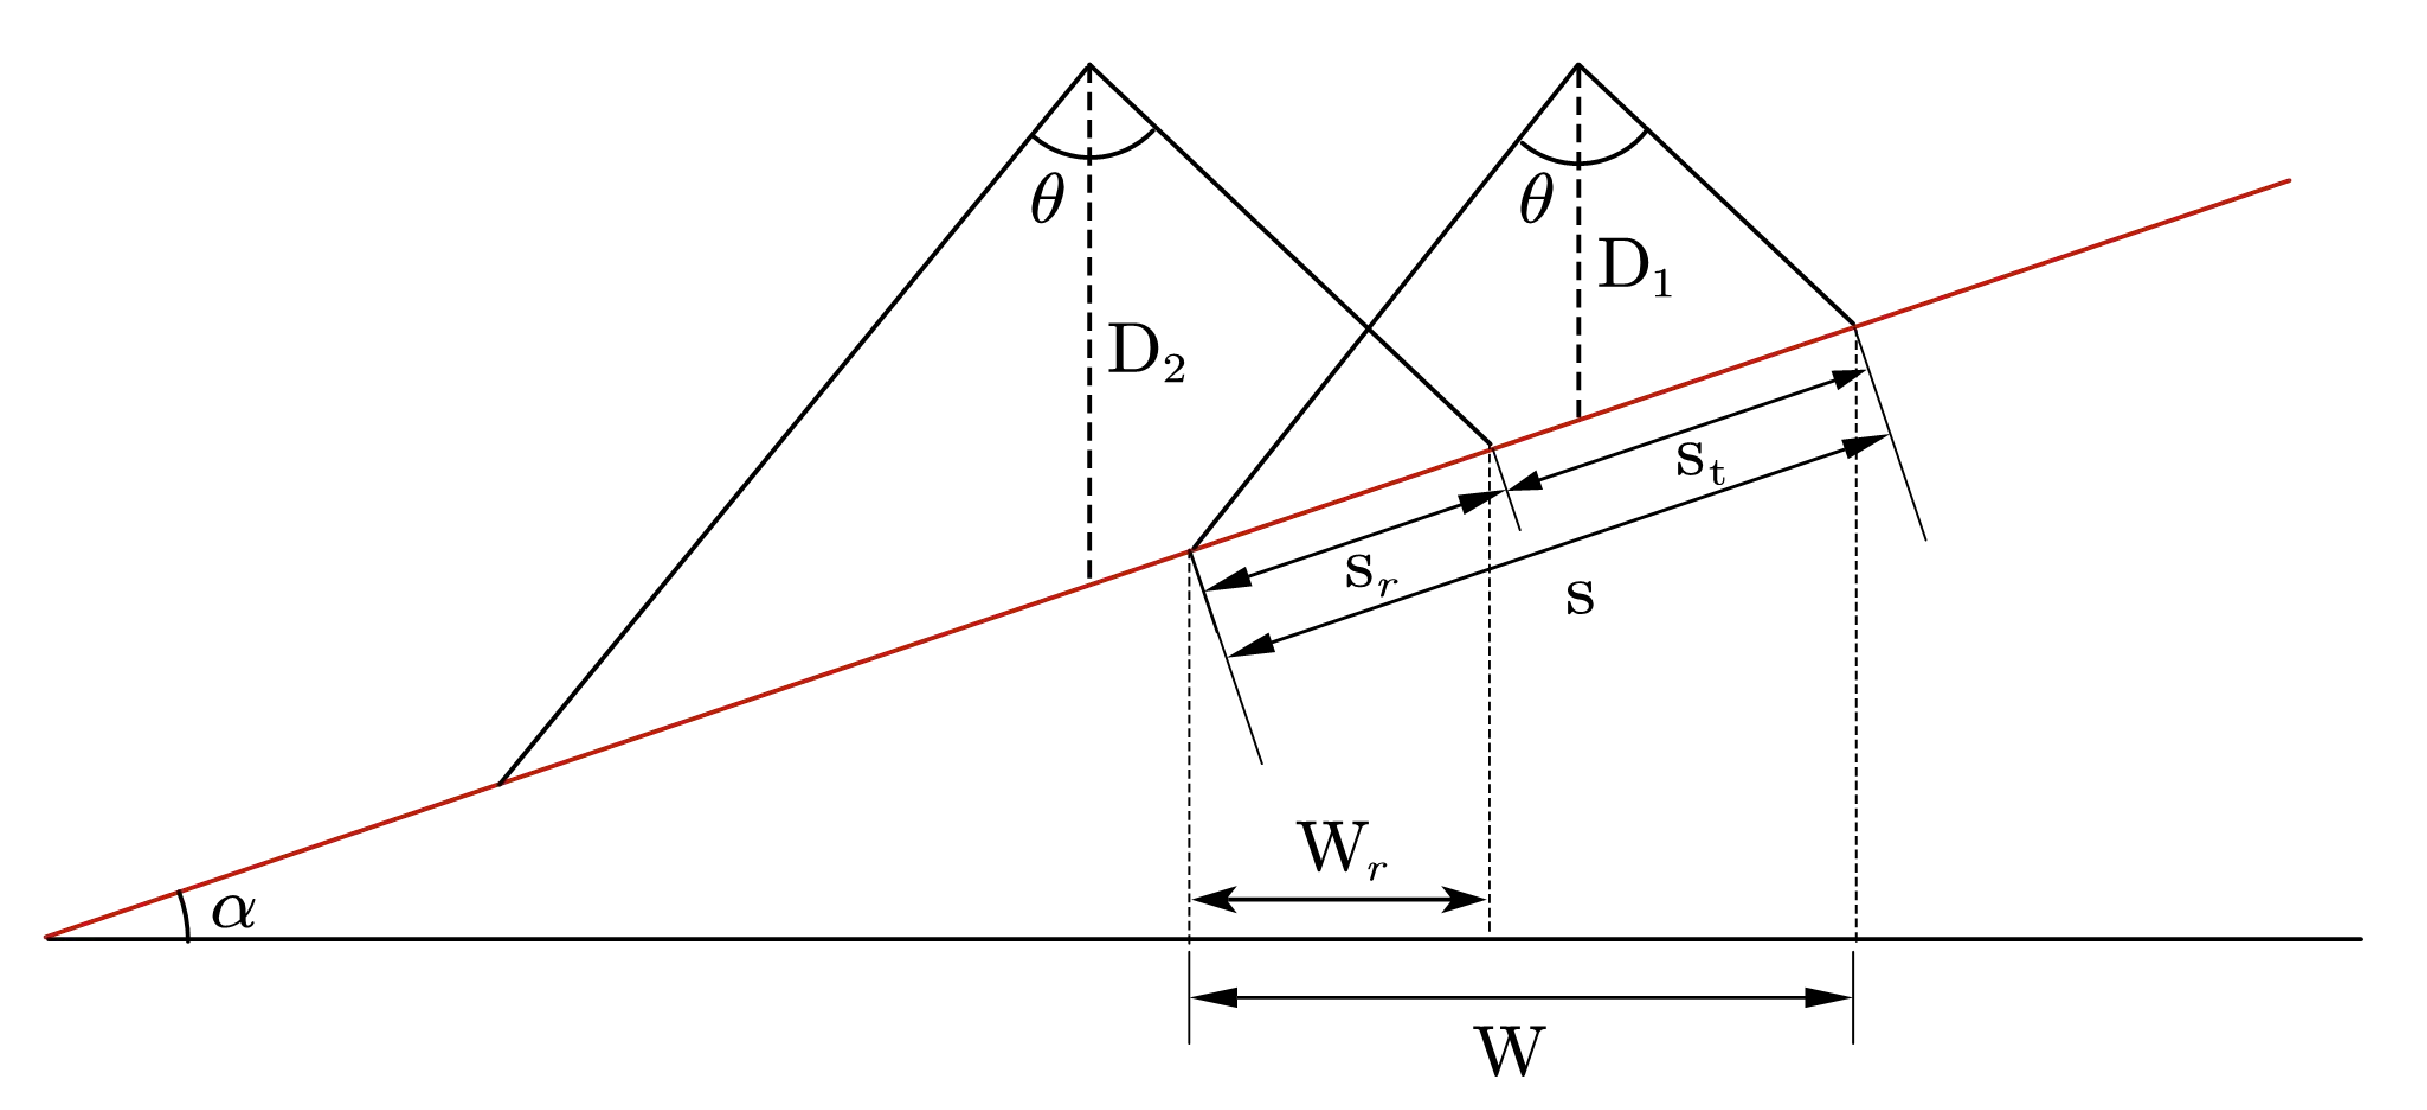
\includegraphics[width=.7\textwidth]{f2}
            \caption{覆盖宽度示例}
            \label{fig:f2}
        \end{figure}
        考虑到两次投影的角度相同,为方便计算,本文用
        \begin{equation}
            \eta=\frac{s_r}{s} = 1-\frac{s_t}{s}
            \label{eq:over_rate}
        \end{equation}
        来计算重叠率。 
        \begin{figure}[H]
            \centering
            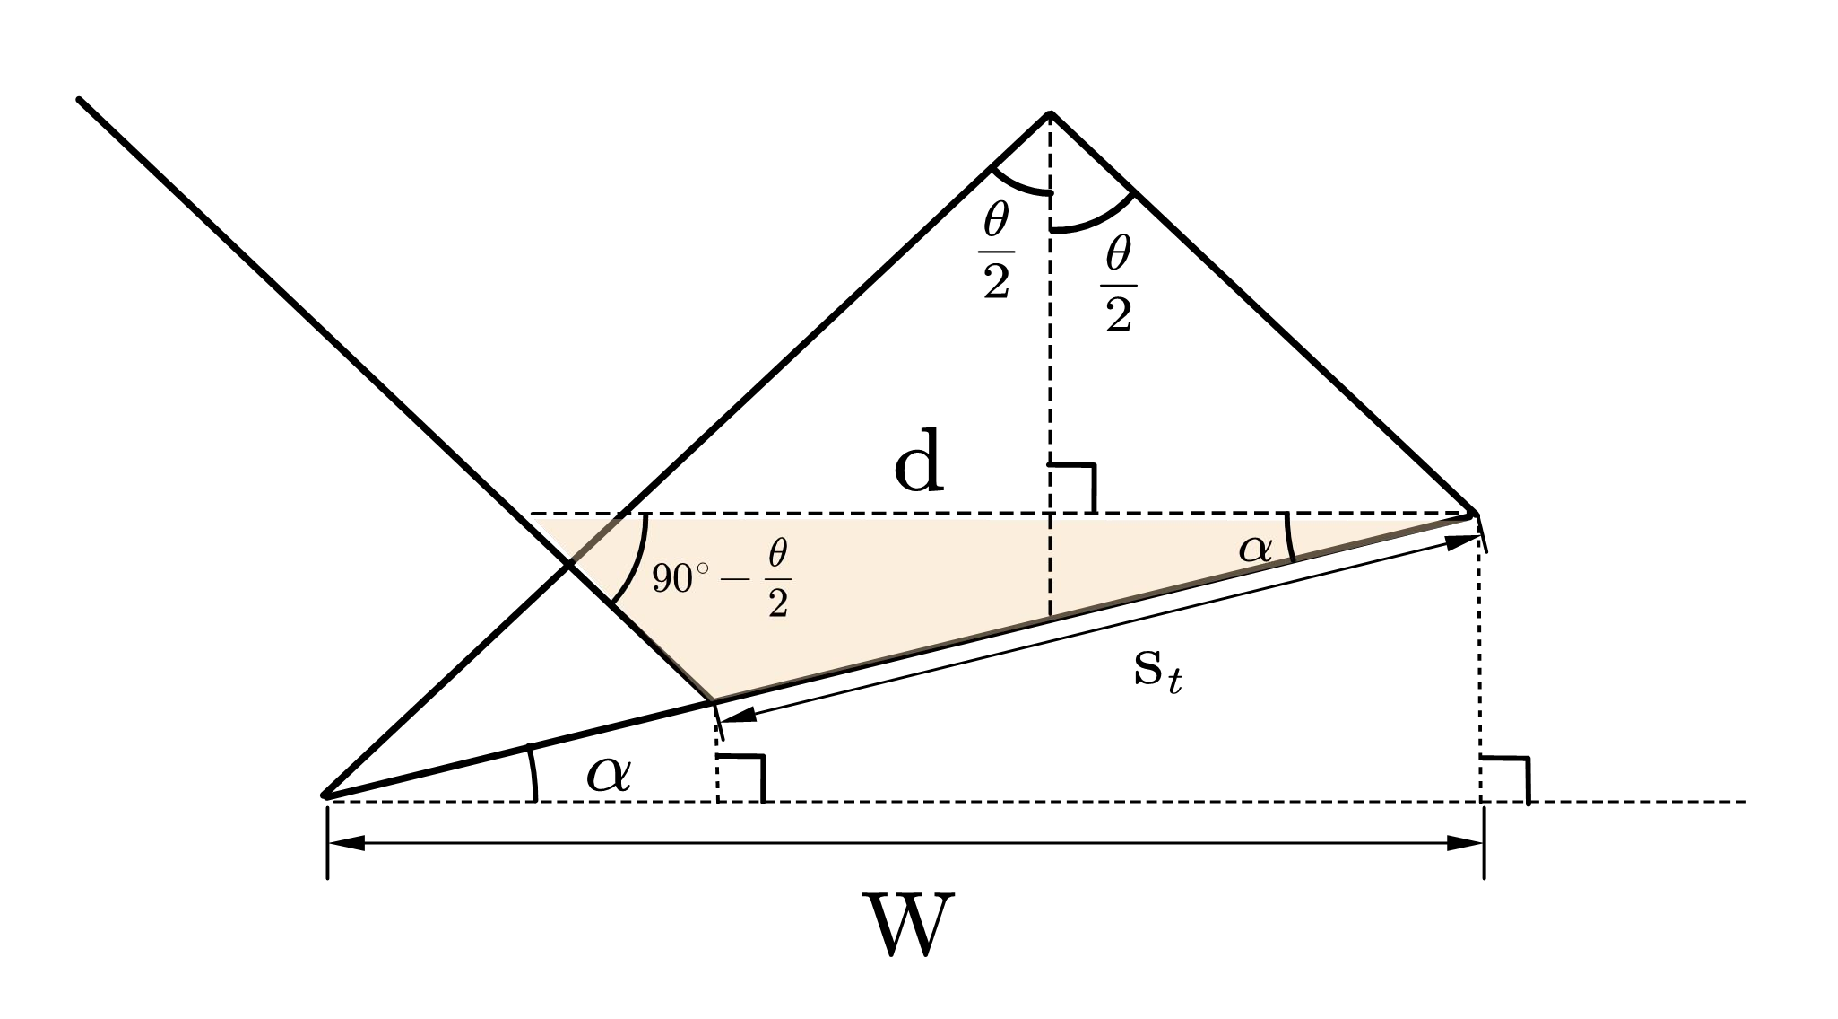
\includegraphics[width=.65\textwidth]{sin}
            \caption{解三角形示意图}
            \label{fig:sin}
        \end{figure}
        对于 $s_r$ 的求解,本文对\cref{fig:sin}所示的三角形采用\textbf{正弦定理}:
        \begin{equation}
            \frac{d}{\sin(\pi - (\frac{\pi}{2}-\frac{\theta}{2})-\alpha)} = \frac{s_t}{\sin(\frac{\pi}{2} - \frac{\theta}{2})}
            \label{eq:sin}
        \end{equation}
        求得 
        \begin{equation}
            s_t = \frac{d\cos\frac{\theta}{2}}{\cos(\alpha-\frac{\theta}{2})}
            \label{eq:solve_s_t}
        \end{equation}
        又因为
        \begin{equation}
            s=\frac{W}{\cos\alpha}
            \label{eq:solve_s}
        \end{equation}
        联立\cref{eq:over_rate}\cref{eq:solve_s_t}\cref{eq:solve_s},可得,覆盖宽度与重叠率的关系为:
        \begin{equation}
            \eta = 1 - \frac{\cos\alpha\cos\frac{\theta}{2}}{\cos(\alpha - \frac{\theta}{2})}\frac{d}{W}
            \label{eq:eta_W}
        \end{equation}
       
        \subsubsection{海底深度、覆盖宽度与重叠率的求解}
        \textbf{海底深度求解}:
        由于题目中已给定海底的坡度角与中心点深度,可用$\tan\alpha$表示海底平面的爬升率,各点离中心点的有向距离 $\Delta x = x - x_0$与爬升率 $\tan \alpha$ 的乘积即为
        该点相对于中心点的海底深度差 $\Delta D$,从而计算该点的海底深度 $D$。即$\Delta D = (x - x_0)\tan\alpha$,$D = D_0 - \Delta D$。
        \begin{figure}[H]
            \centering
            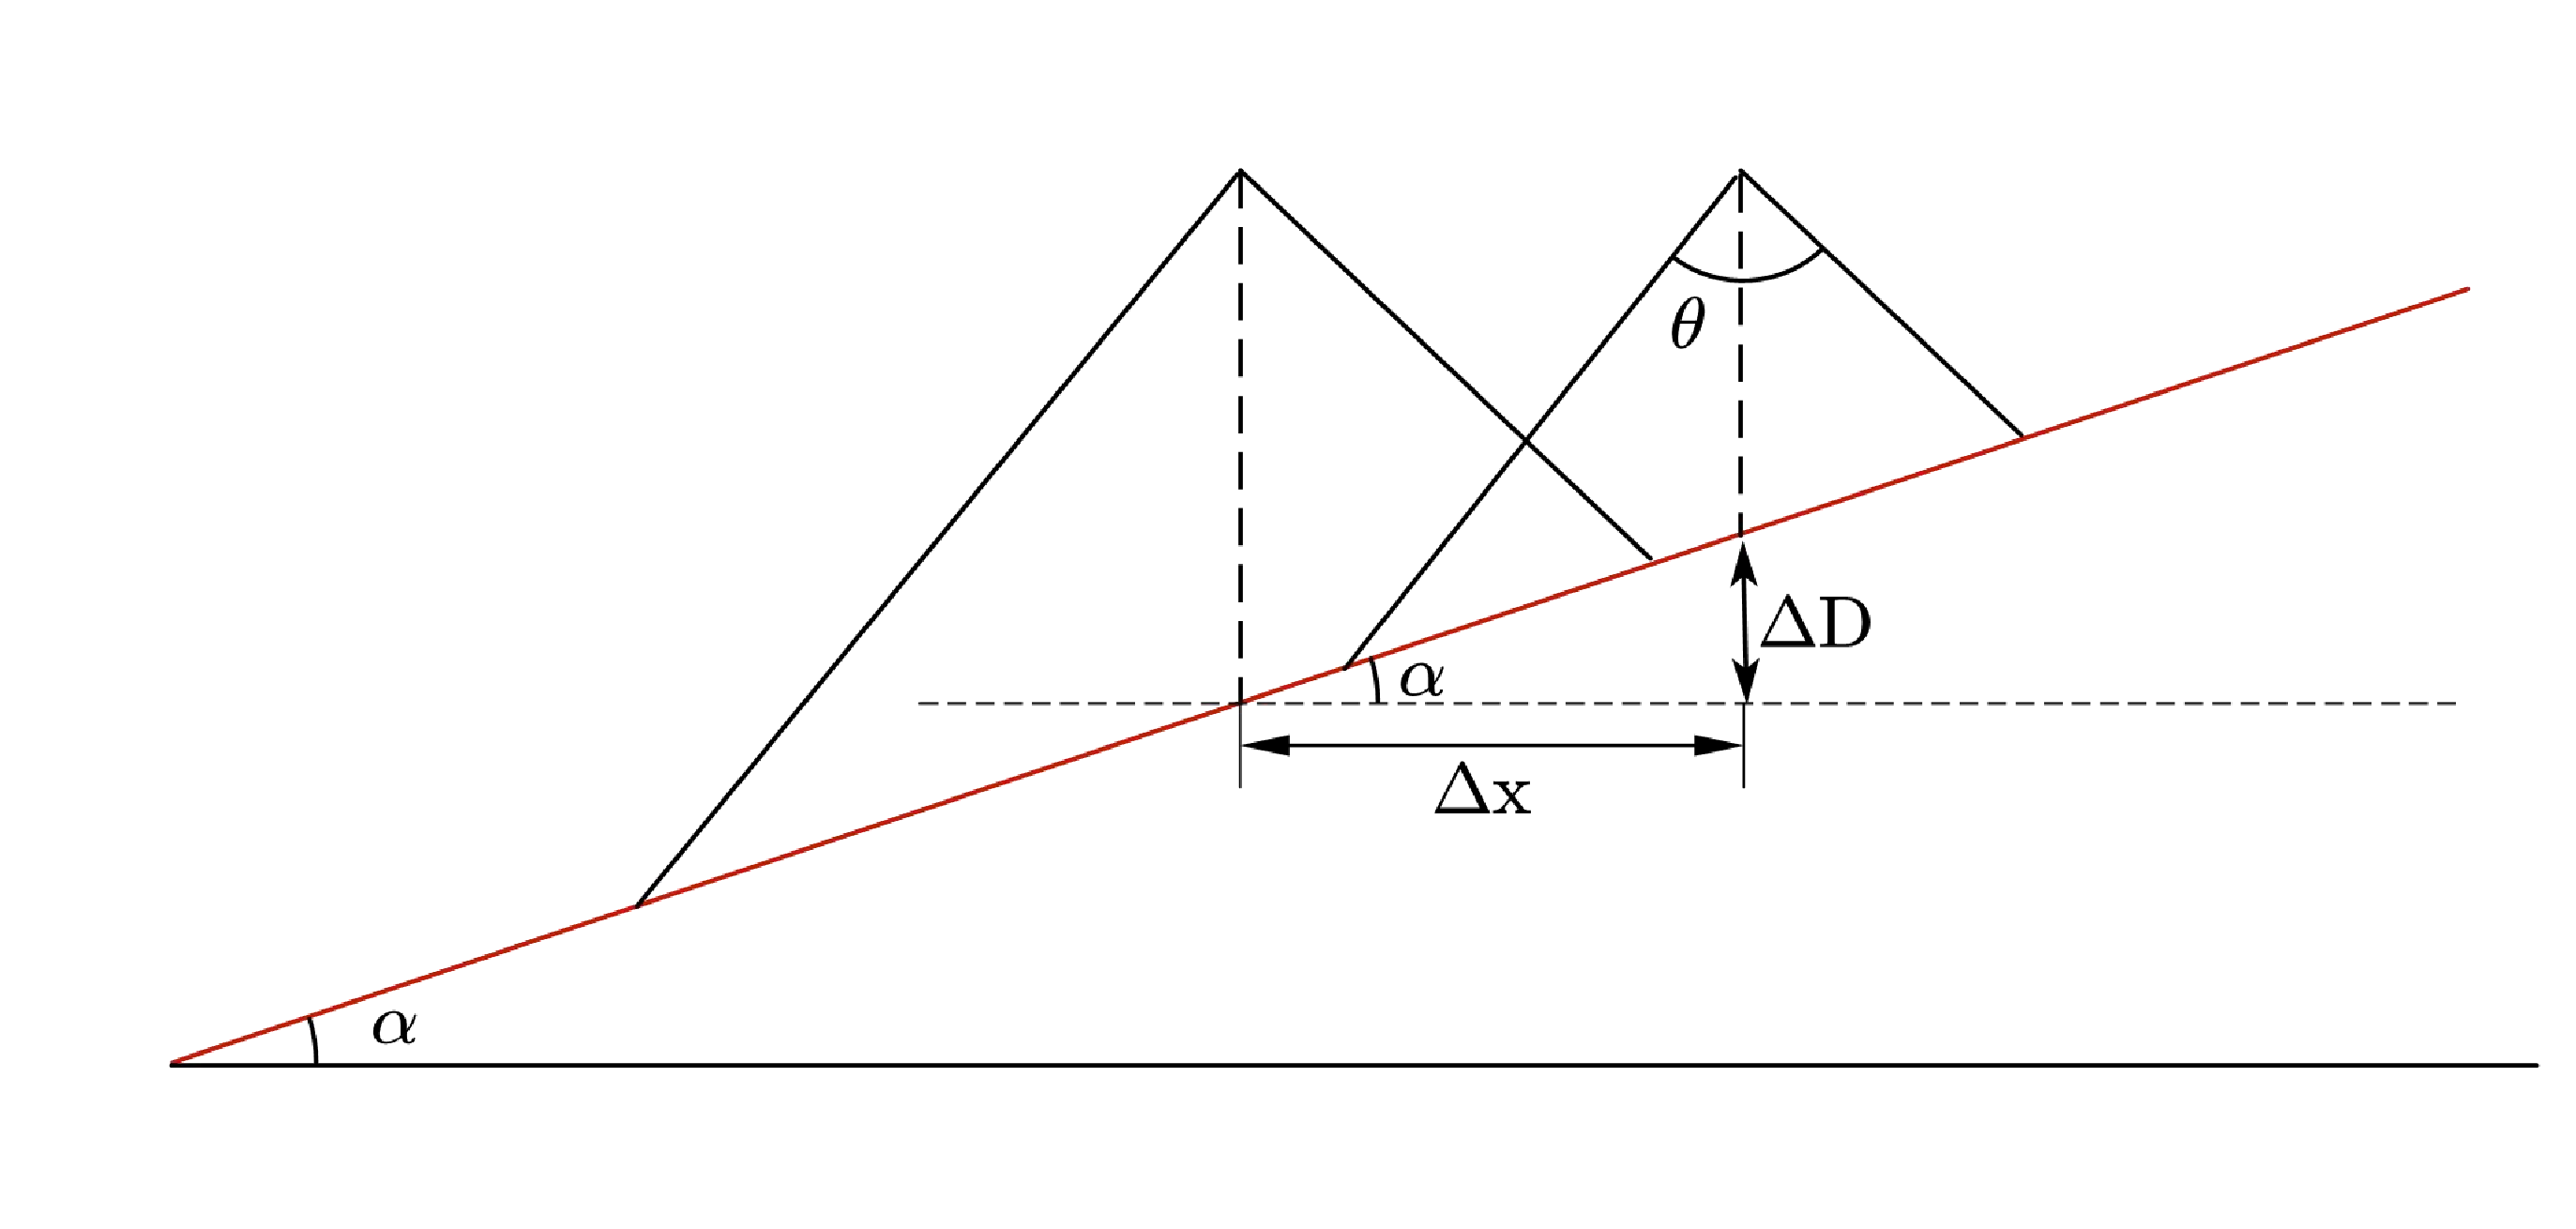
\includegraphics[width=.6\textwidth]{f1}
            \caption{海底深度求解示意图}
            \label{fig:f1}
        \end{figure}

        \textbf{覆盖宽度求解}:
        \begin{figure}[!htbp]
            \centering
            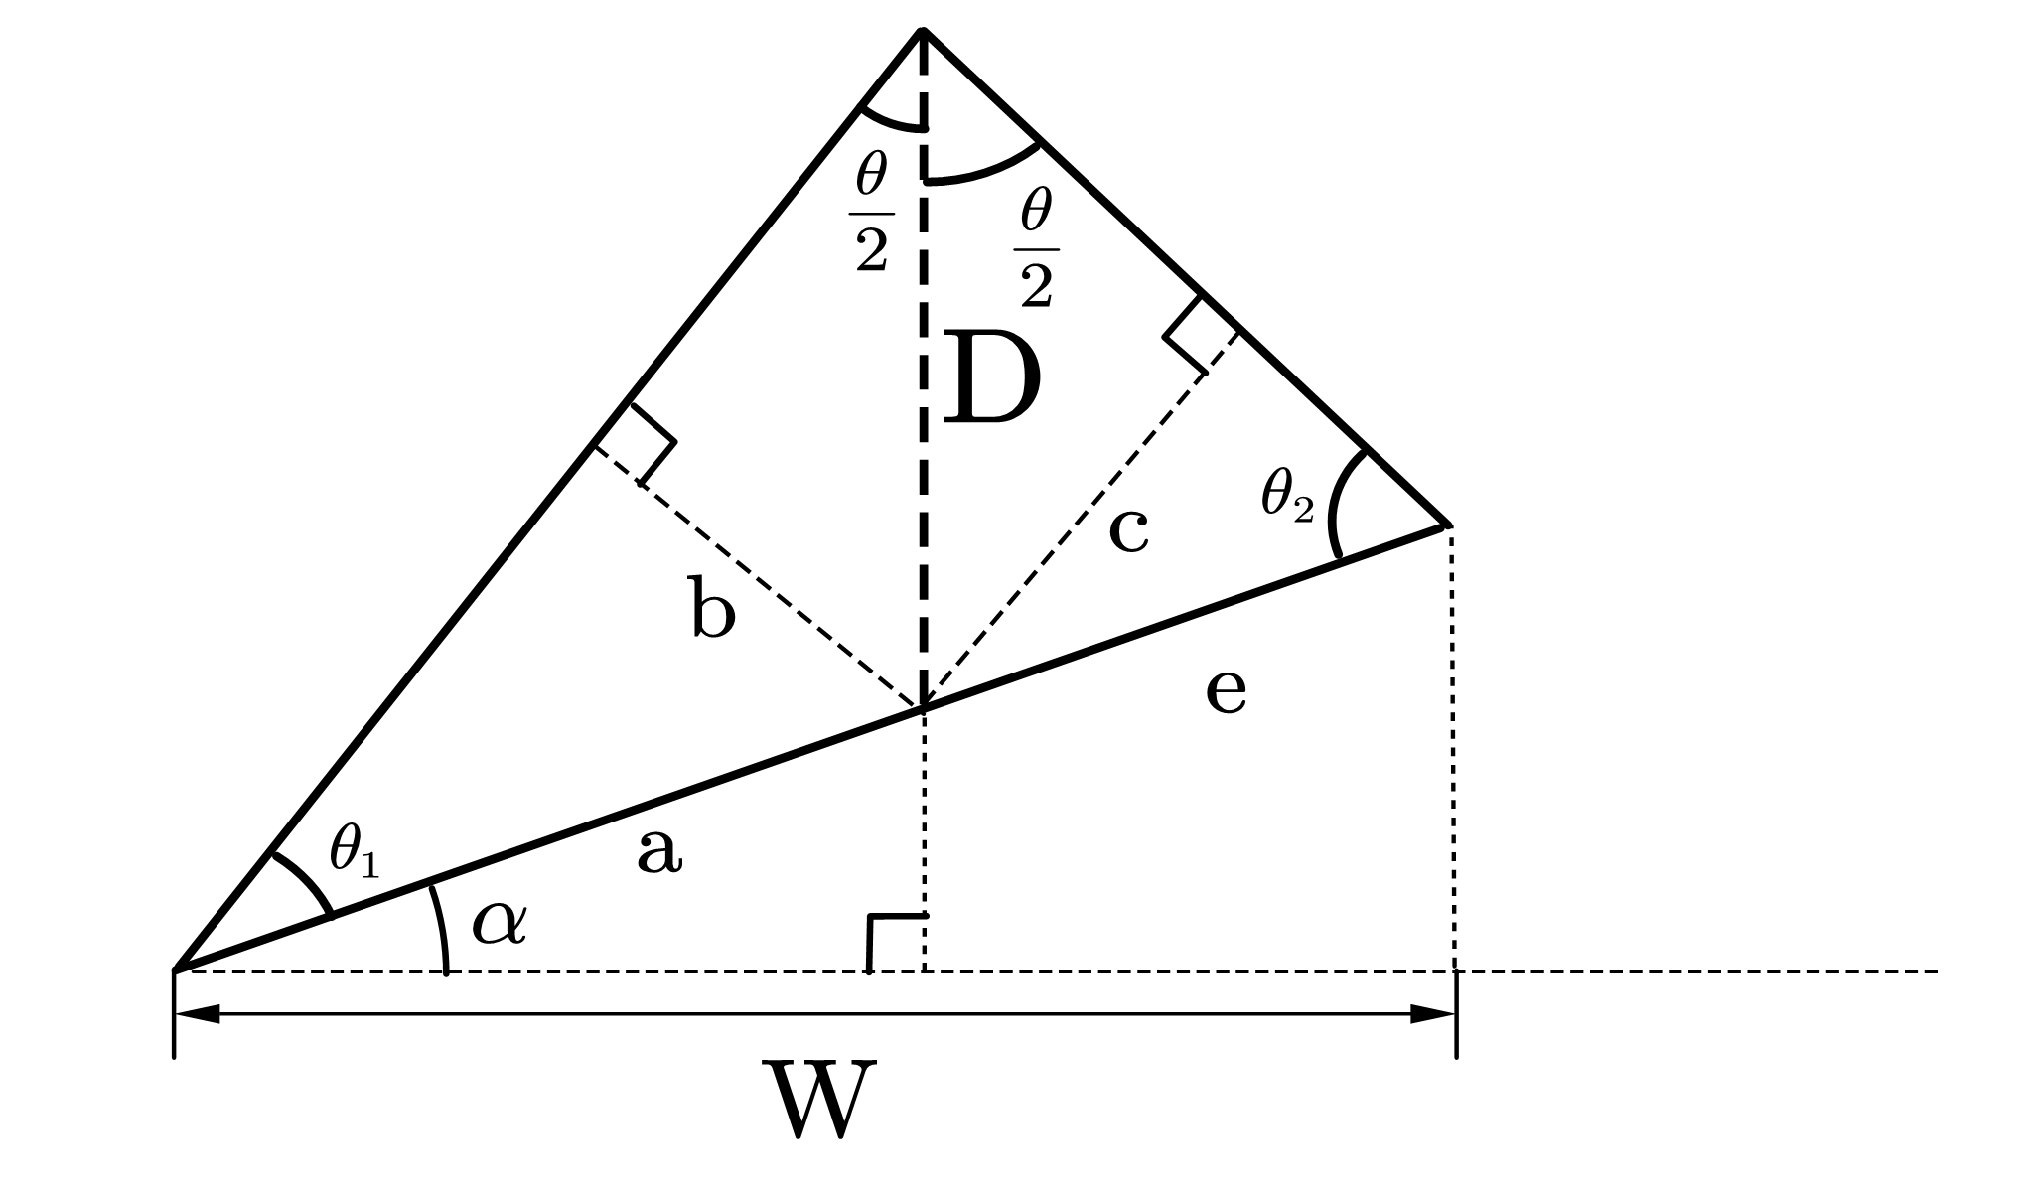
\includegraphics[width=.7\textwidth]{W1}
            \caption{角平分线定理示意图}
            \label{fig:}
        \end{figure}
        本文利用了波束的对称性,可利用角平分线简化覆盖宽度的计算:
        \begin{equation}
            \begin{cases}
                \theta_1 = 90^{\circ} - \alpha - \frac{\theta}{2} \\
                \theta_2 = 90^{\circ} + \alpha - \frac{\theta}{2} \\
                b = D\sin\frac{\theta}{2} \\
                c = D\sin\frac{\theta}{2} \\
                a = \frac{b}{\sin\theta_1} \\
                e = \frac{c}{\sin\theta_2} \\
                W = (a + e)\cos \alpha
            \end{cases}
            \label{eq:solve_over_width}
        \end{equation}
        可得覆盖宽度的表达式为:
        \begin{equation}
            W = D\sin\frac{\theta}{2}(\frac{1}{\cos(\frac{\theta}{2}+\alpha)} + \frac{1}{\cos(\frac{\theta}{2} - \alpha)})\cos\alpha
            \label{eq:over_width_1}
        \end{equation}

        重叠率求解:
        使用前文建立的覆盖宽度-重叠率模型, 将测线上各个位置的覆盖宽度 $W$ 带入模型
        即可求得测线上各个位置的重叠率 $\eta$。

        \subsubsection{求解结果}
        最终答案如下:
        \begin{table}[H]
            \setlength{\tabcolsep}{3.5pt}
            \centering
            \caption{问题一的计算结果}  
            \label{table:1} 
            \begin{tabular}{|m{2.6cm}|c|c|c|c|c|c|c|c|c|}   
            \hline 测线距中心点处的距离/m\centering & -800 & -600 & -400 & -200 & 0 & 200 & 400 & 600 & 800 \\
            \hline 海水深度/m\centering & 90.95 & 85.71 & 80.47 & 75.24 & 70.00 & 64.76 & 59.53 & 54.29 & 49.05 \\
            \hline 覆盖宽度/m\centering & 315.71 & 297.53 & 279.35 & 261.17 & 242.99 & 224.81 & 206.63 & 188.45 & 170.27 \\
            \hline 与前一条测线的重叠率/\%\centering & - & 35.69 & 31.51 & 26.74 & 21.26 & 14.89 & 7.41 & -1.53 & -12.36 \\
            \hline
            \end{tabular}       
        \end{table}

        由求解结果可知,在坡度一定的情况下,随着海水深度 $D$ 的增加,覆盖宽度 $W$ 也相应的增加,重叠率 $\eta$ 也增加。

        \subsection{问题二模型的建立与求解}
        求解问题二主要需要两个步骤:(1)将三维空间中的问题转化为平面解三角形问题;(2)通过解三角形求出各点覆盖宽度。
        \subsubsection{坐标系的建立}
        \begin{figure}[H]
            \centering
            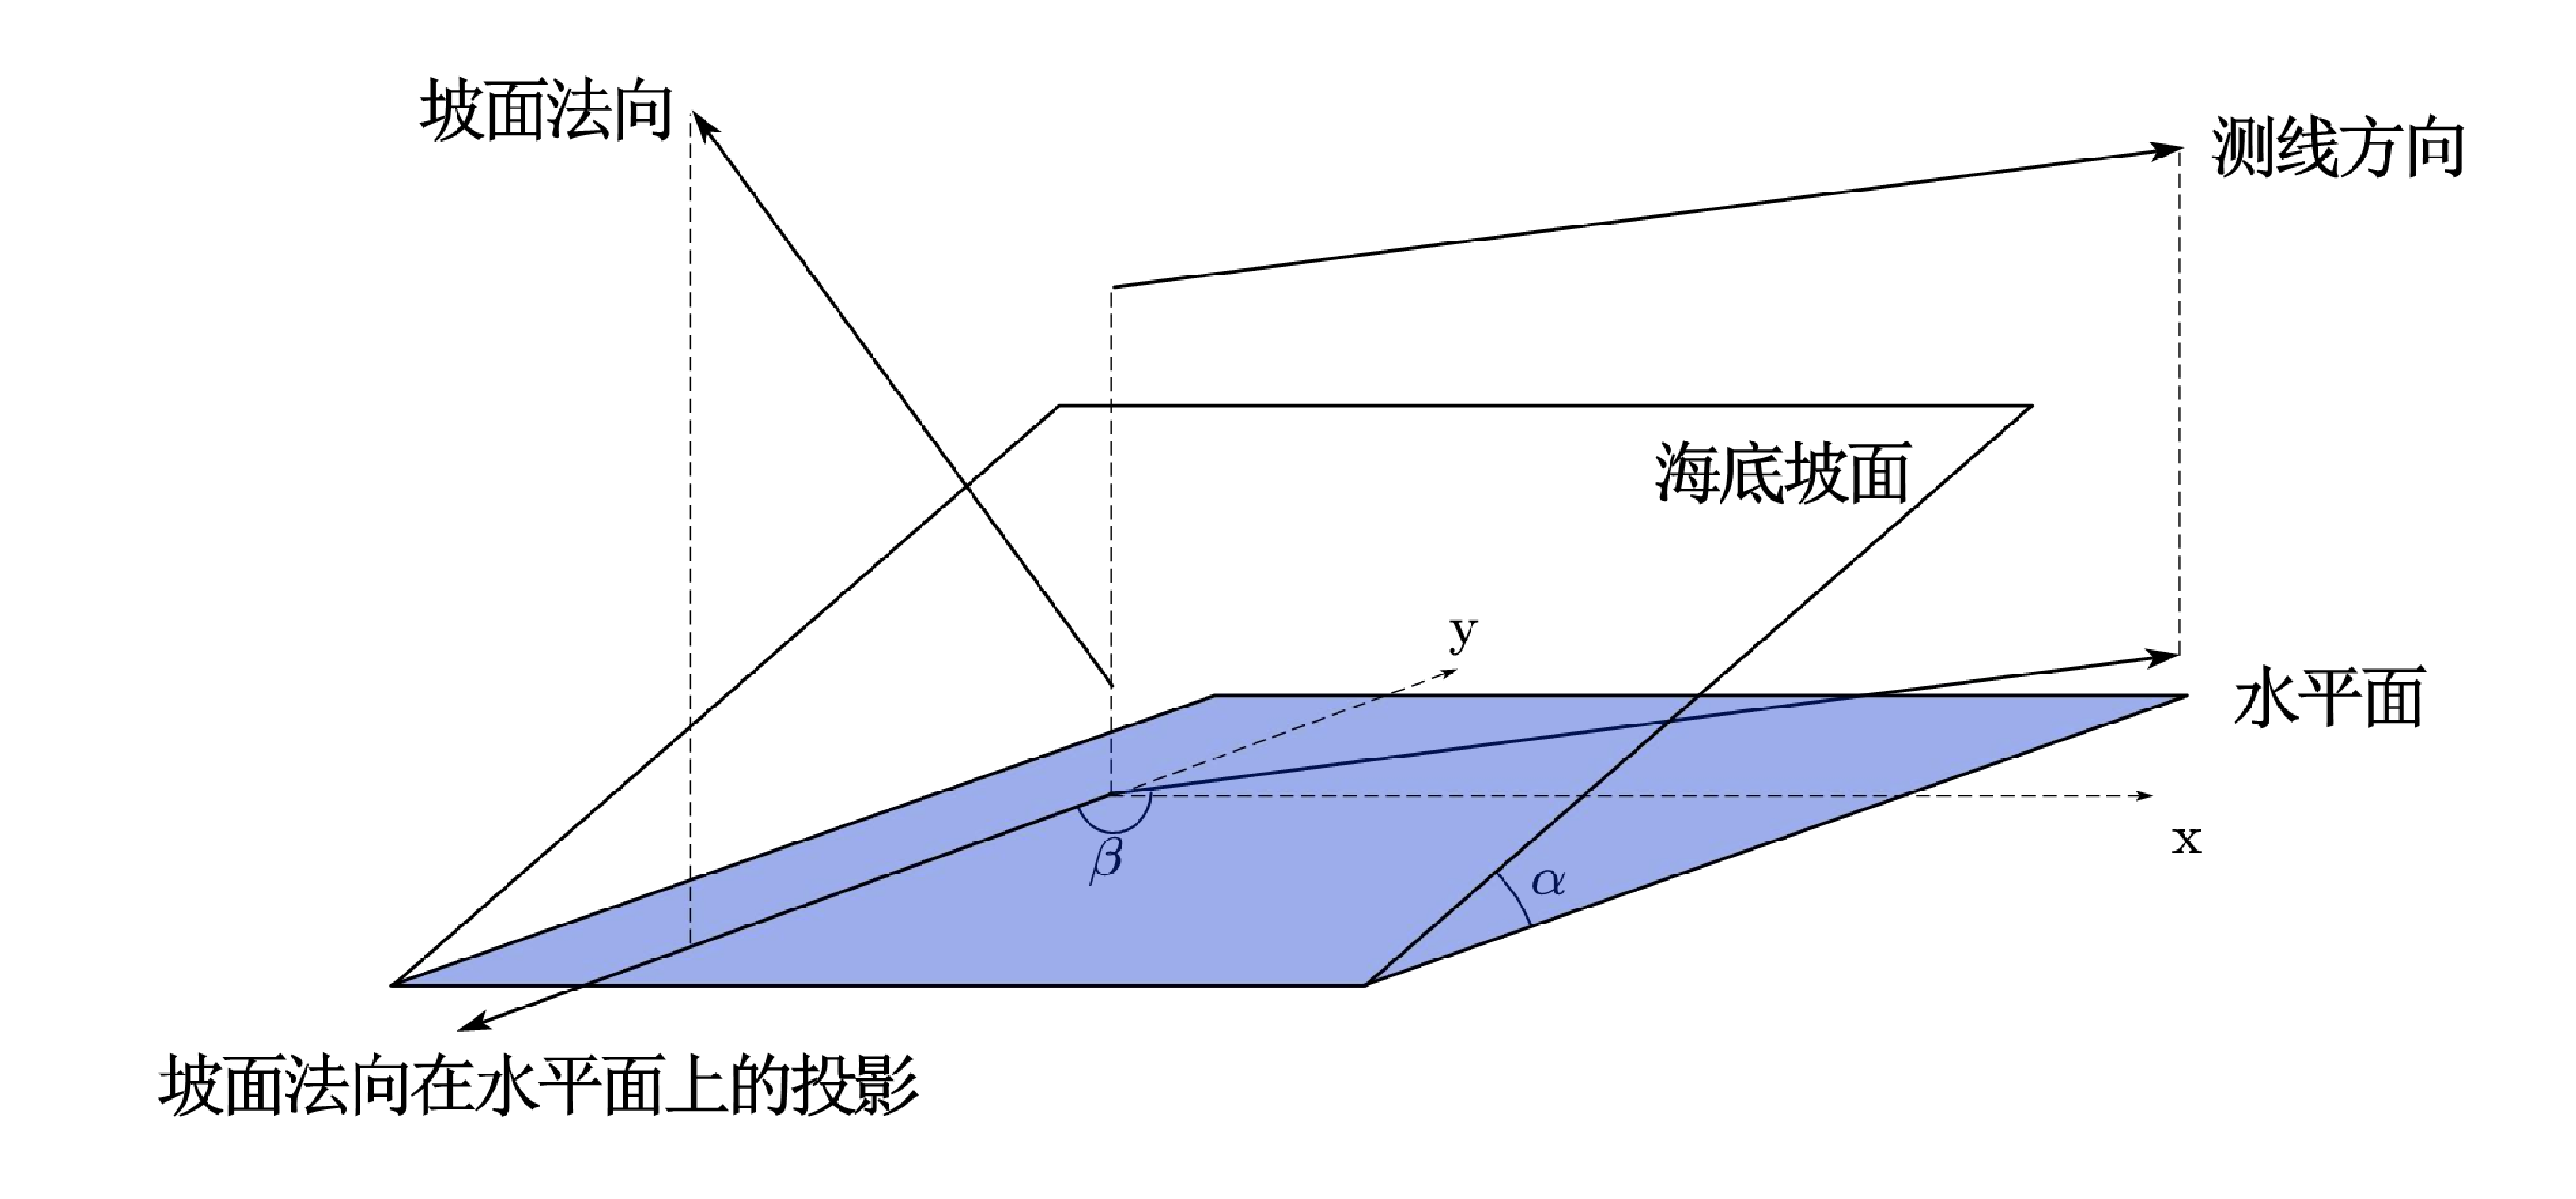
\includegraphics[width=.9\textwidth]{f4}
            \caption{坐标系的建立}
            \label{fig:f4}
        \end{figure}
        如图,以等深线方向为$x$轴,以坡度升高方向为y轴正方向,建立直角坐标系。
        特别地,称$y$轴为坡度方向。

        \subsubsection{海底爬升率的计算}
        \begin{figure}[H]
            \centering
            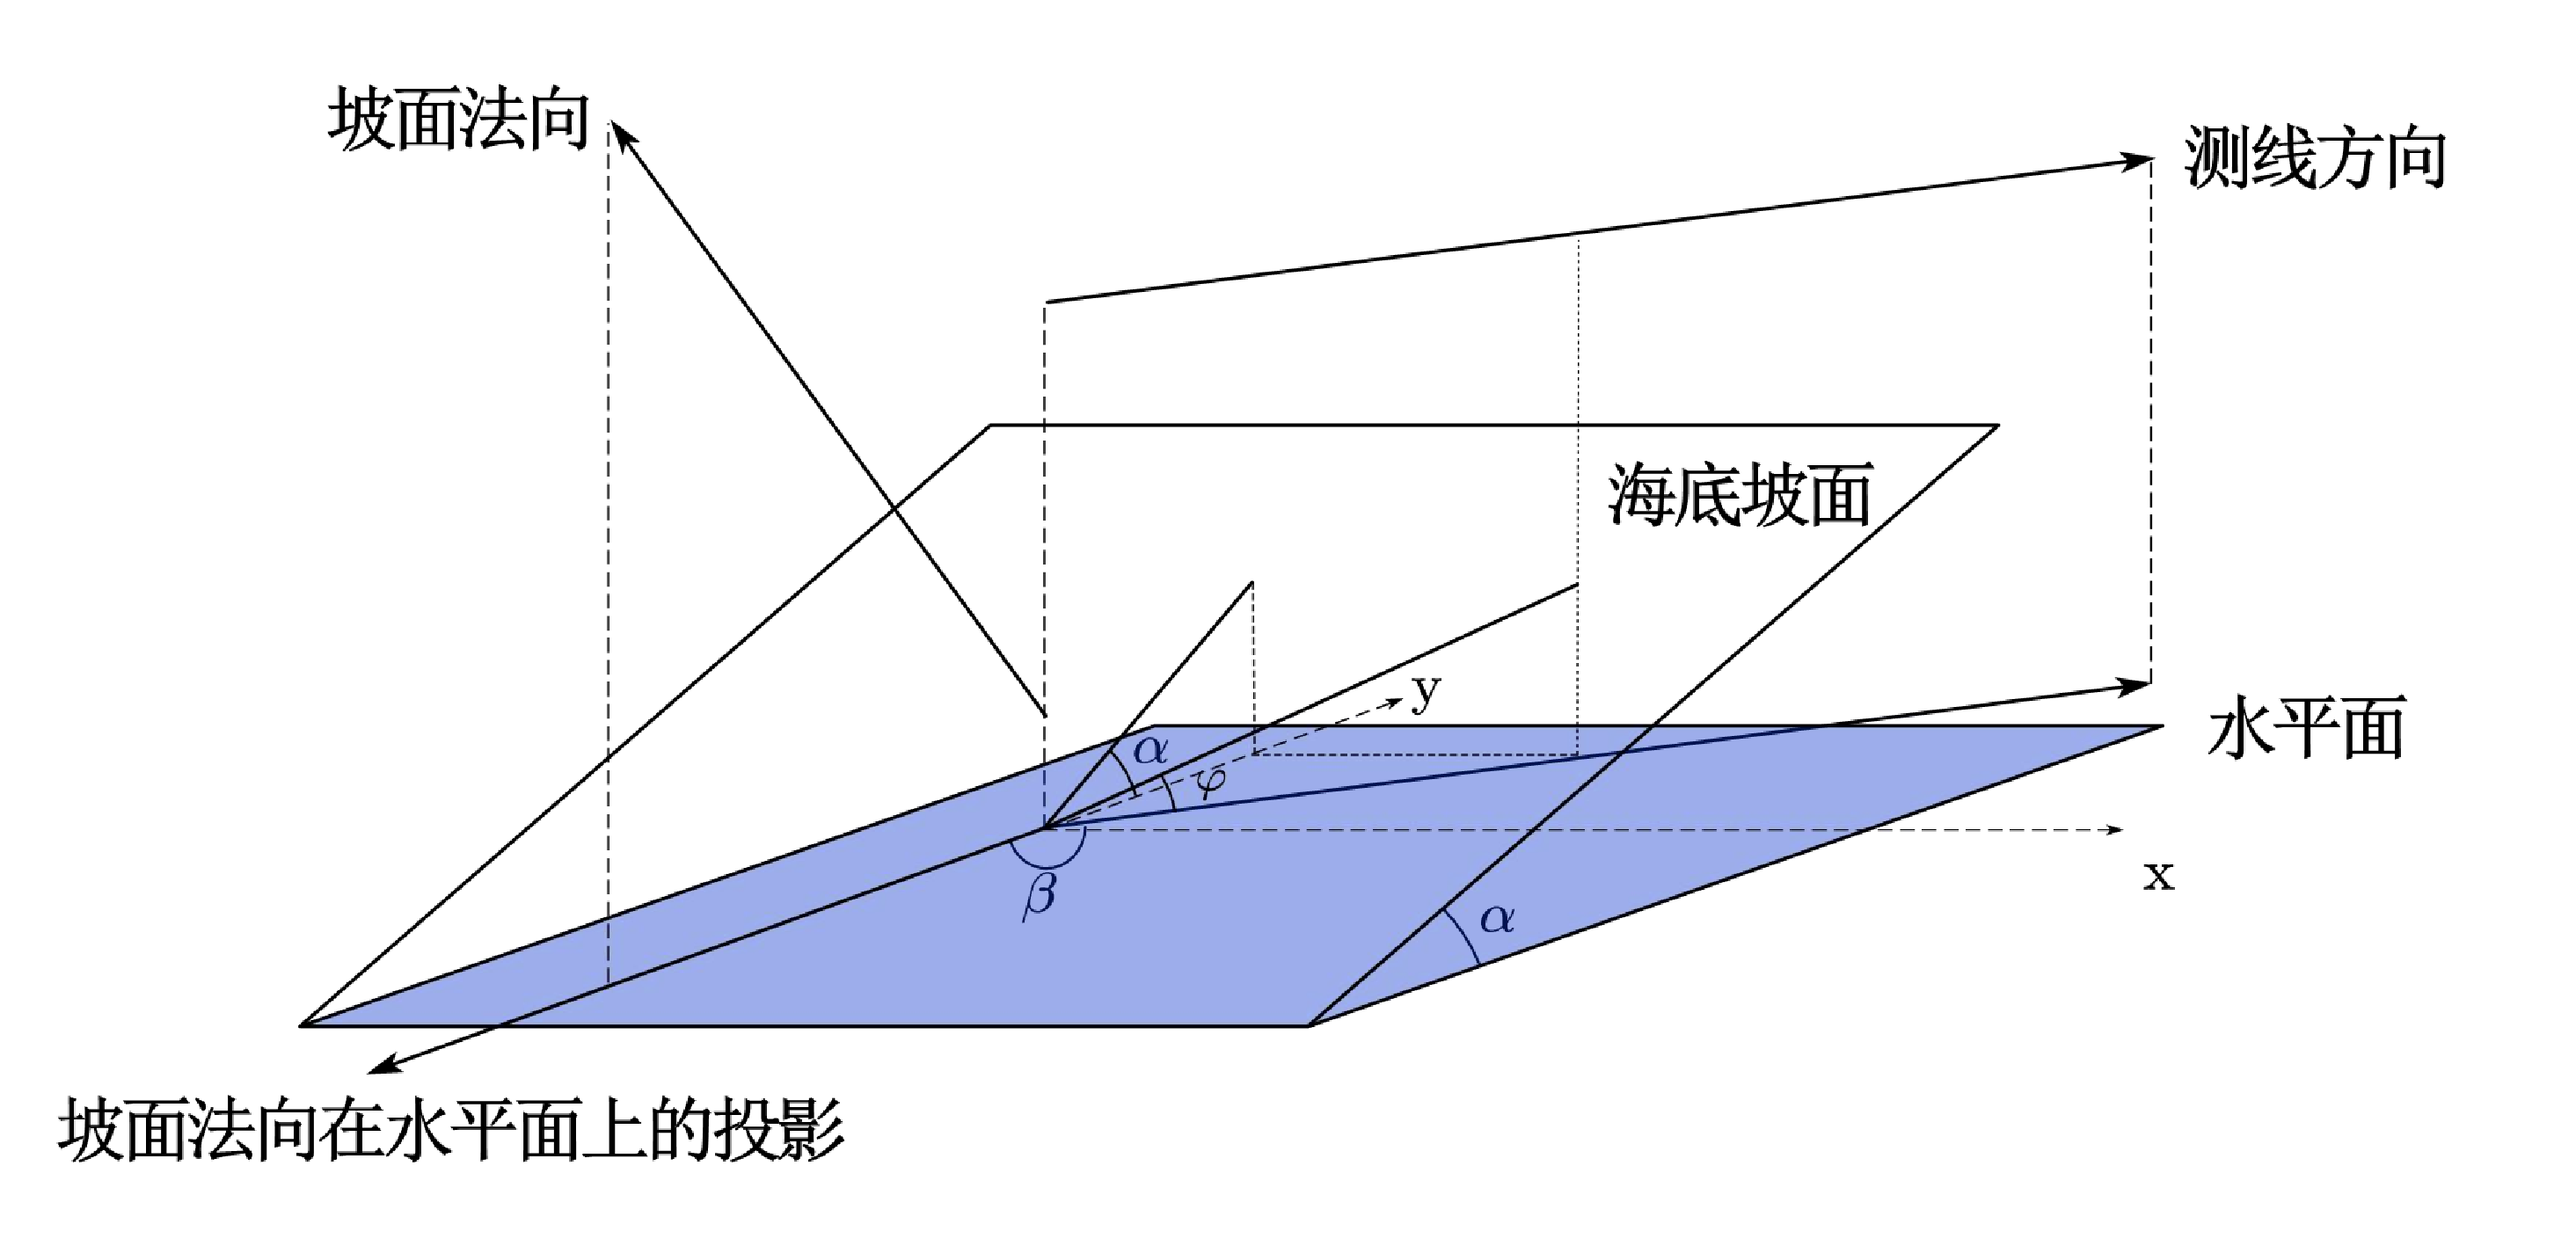
\includegraphics[width=.9\textwidth]{varphi}
            \caption{测线方向爬升角示意图}
            \label{fig:varphi}
        \end{figure}
        考虑到测线与坡度方向有夹角,可先将测线方向分解到平行坡度方向与垂直坡度方向。已知垂直坡度方向的部分对海底的高度变化无贡献,故只需考虑
        平行坡度方向的部分带来的高度变化,该方向上的爬升率可以用$\tan\alpha $表示。因此,沿测线爬升率可用公式$\tan\varphi = -\cos\beta \tan\alpha $表示,其中称$\varphi$为爬升角。
        
        \subsubsection{覆盖宽度的求解}
        \begin{figure}[H]
            \centering
            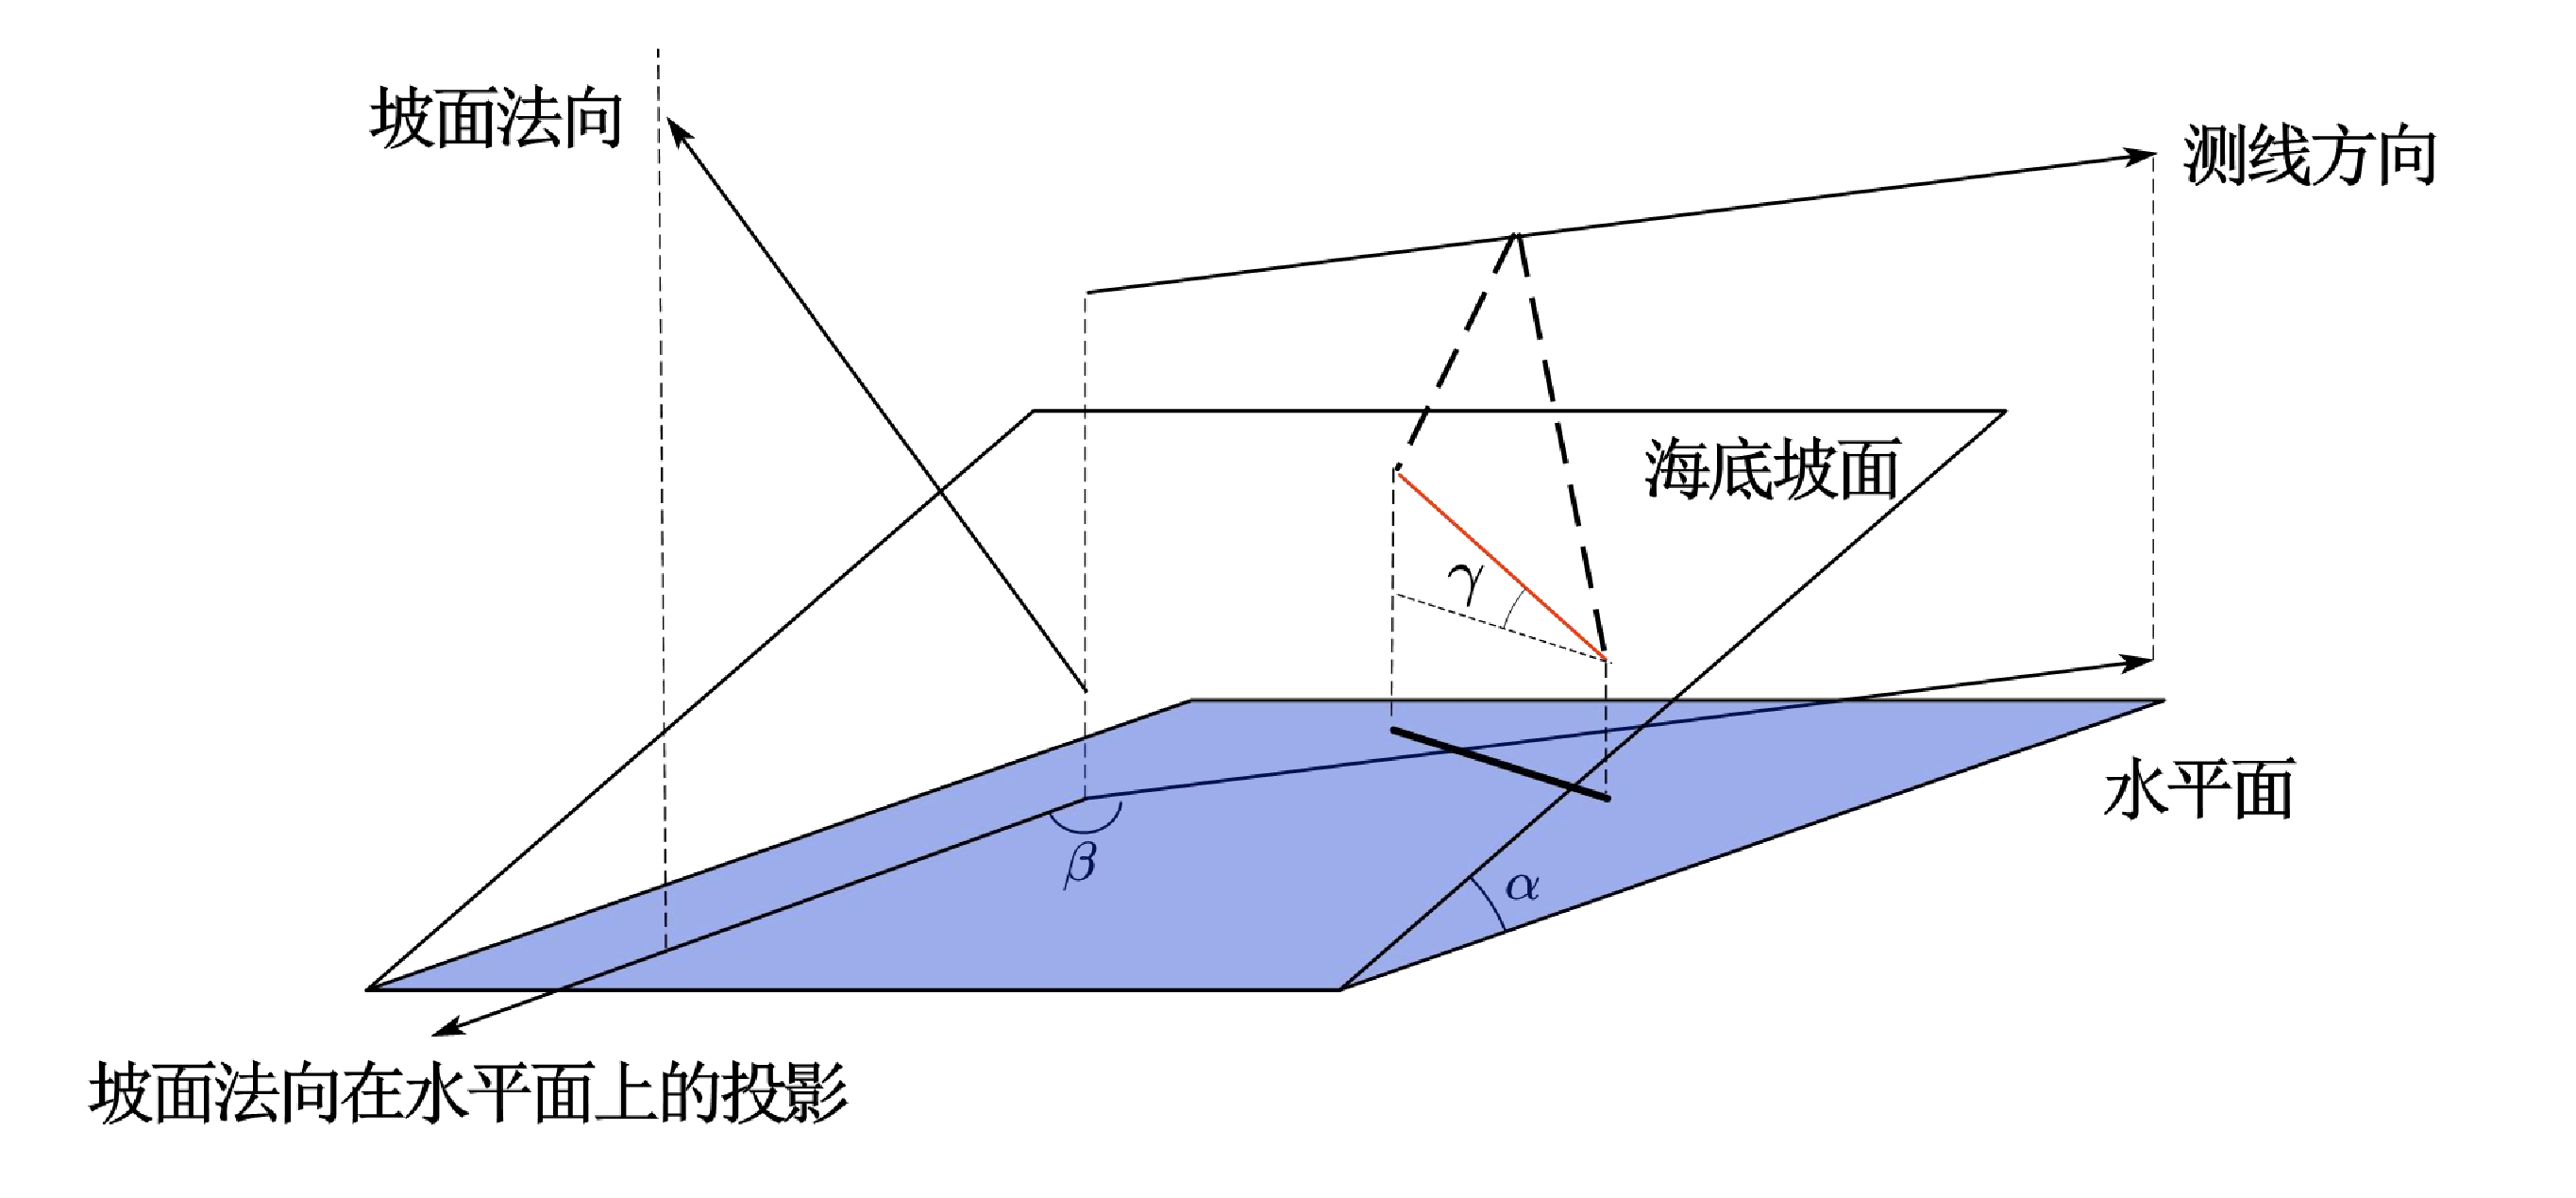
\includegraphics[width=.9\textwidth]{gamma}
            \caption{垂直测线方向爬升角示意图}
            \label{fig:gamma1}
        \end{figure}
        本文先将覆盖宽度 $W$ 的求解转化为解三角形问题,可先确定$\gamma$的值,从而得到三角形各角角度,再沿用问题一中的简化方法求解。

        求解$\gamma$等价于求解覆盖宽度所在边的爬升率,则仍可沿用前文中爬升率计算的方法,将覆盖宽度分解到平行坡度方向与垂直坡度方向,
        得$\tan\gamma = \sin\beta \tan\alpha $。
        \begin{figure}[H]
            \centering
            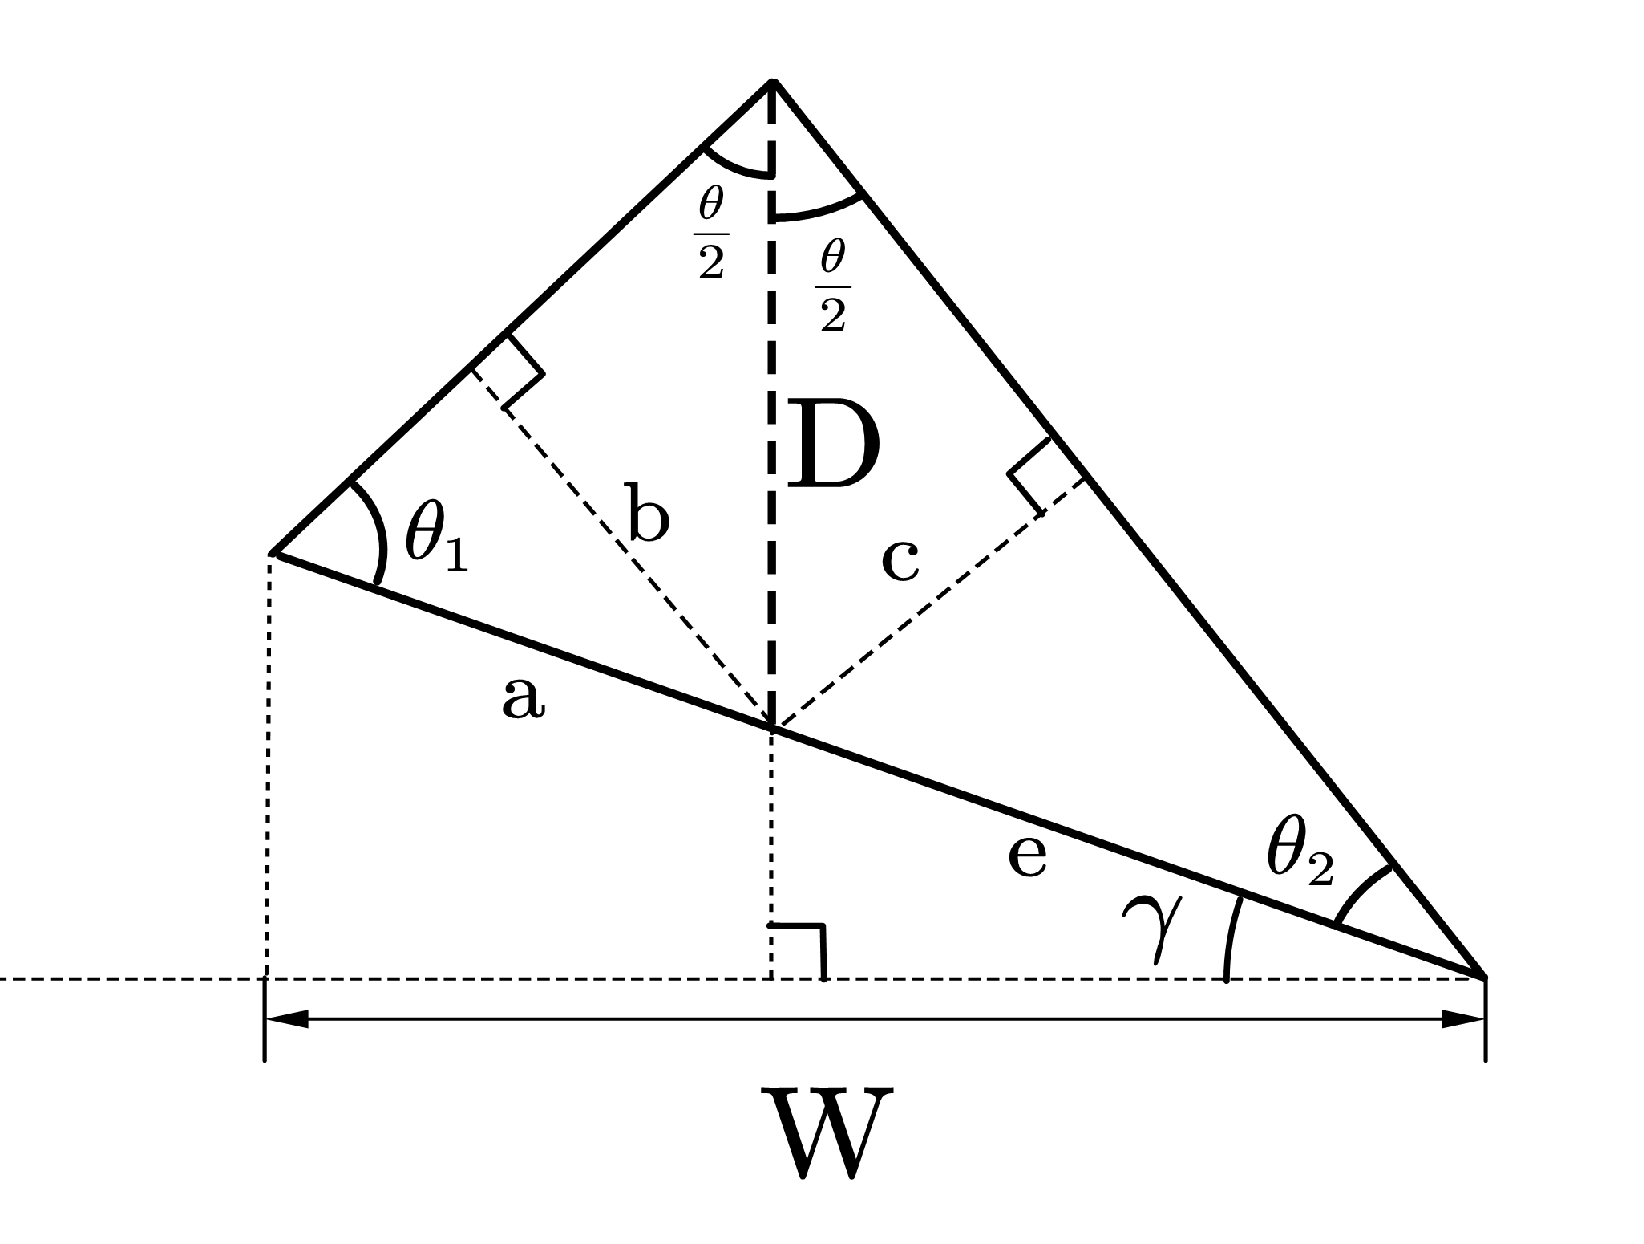
\includegraphics[width=.6\textwidth]{W2}
            \caption{角平分线定理示意图}
            \label{fig:W2}
        \end{figure}
        沿用问题一中方法,可得覆盖宽度的表达式为
        \begin{equation}
            W = D\sin\frac{\theta}{2}(\frac{1}{\cos(\frac{\theta}{2}+\gamma)} + \frac{1}{\cos(\frac{\theta}{2} - \gamma)})\cos\gamma
            \label{eq:over_width_2}
        \end{equation}
        
        \subsubsection{求解结果}
        最终答案如下:
        \begin{table}[H]
            \caption{问题二的计算结果}
            \label{table:2}
            \begin{center}
            \begin{tabular}{|cc|cccccccc|}
            \hline
            \multicolumn{2}{|c|}{\multirow{2}{*}{覆盖宽度/m}}         & \multicolumn{8}{c|}{测量船距海域中心点处的距离/海里}                                                                                                                                                          \\ \cline{3-10} 
            \multicolumn{2}{|c|}{}                                & \multicolumn{1}{c|}{0} & \multicolumn{1}{c|}{0.3} & \multicolumn{1}{c|}{0.6} & \multicolumn{1}{c|}{0.9} & \multicolumn{1}{c|}{1.2} & \multicolumn{1}{c|}{1.5} & \multicolumn{1}{c|}{1.8} & 2.1 \\ \hline
            \multicolumn{1}{|c|}{\multirow{8}{*}{\makecell[c]{测线\\方向\\夹角\\/$^{\circ}$}}} & 0   & \multicolumn{1}{c|}{415.69}  & \multicolumn{1}{c|}{466.09}    & \multicolumn{1}{c|}{516.49}    & \multicolumn{1}{c|}{566.89}    & \multicolumn{1}{c|}{617.29}    & \multicolumn{1}{c|}{667.69}    & \multicolumn{1}{c|}{718.09}    &  768.48  \\ \cline{2-10} 
            \multicolumn{1}{|c|}{}                          & 45  & \multicolumn{1}{c|}{416.12}  & \multicolumn{1}{c|}{451.79}    & \multicolumn{1}{c|}{487.47}    & \multicolumn{1}{c|}{523.14}    & \multicolumn{1}{c|}{558.82}    & \multicolumn{1}{c|}{594.49}    & \multicolumn{1}{c|}{630.16}    &   665.84  \\ \cline{2-10} 
            \multicolumn{1}{|c|}{}                          & 90  & \multicolumn{1}{c|}{416.55}  & \multicolumn{1}{c|}{416.55}    & \multicolumn{1}{c|}{416.55}    & \multicolumn{1}{c|}{416.55}    & \multicolumn{1}{c|}{416.55}    & \multicolumn{1}{c|}{416.55}    & \multicolumn{1}{c|}{416.55}    &   416.55  \\ \cline{2-10} 
            \multicolumn{1}{|c|}{}                          & 135 & \multicolumn{1}{c|}{416.12}  & \multicolumn{1}{c|}{380.45}    & \multicolumn{1}{c|}{344.77}    & \multicolumn{1}{c|}{309.10}    & \multicolumn{1}{c|}{273.42}    & \multicolumn{1}{c|}{237.75}    & \multicolumn{1}{c|}{202.08}    &   166.40  \\ \cline{2-10} 
            \multicolumn{1}{|c|}{}                          & 180 & \multicolumn{1}{c|}{415.69}  & \multicolumn{1}{c|}{365.29}    & \multicolumn{1}{c|}{314.89}    & \multicolumn{1}{c|}{264.50}    & \multicolumn{1}{c|}{214.10}    & \multicolumn{1}{c|}{163.70}    & \multicolumn{1}{c|}{113.30}    &   62.90  \\ \cline{2-10} 
            \multicolumn{1}{|c|}{}                          & 225 & \multicolumn{1}{c|}{416.12}  & \multicolumn{1}{c|}{380.45}    & \multicolumn{1}{c|}{344.77}    & \multicolumn{1}{c|}{309.10}    & \multicolumn{1}{c|}{273.42}    & \multicolumn{1}{c|}{237.75}    & \multicolumn{1}{c|}{202.08}    &   166.40  \\ \cline{2-10} 
            \multicolumn{1}{|c|}{}                          & 270 & \multicolumn{1}{c|}{416.55}  & \multicolumn{1}{c|}{416.55}    & \multicolumn{1}{c|}{416.55}    & \multicolumn{1}{c|}{416.55}    & \multicolumn{1}{c|}{416.55}    & \multicolumn{1}{c|}{416.55}    & \multicolumn{1}{c|}{416.55}    &   416.55  \\ \cline{2-10} 
            \multicolumn{1}{|c|}{}                          & 315 & \multicolumn{1}{c|}{416.12}  & \multicolumn{1}{c|}{451.79}    & \multicolumn{1}{c|}{487.47}    & \multicolumn{1}{c|}{523.14}    & \multicolumn{1}{c|}{558.82}    & \multicolumn{1}{c|}{594.49}    & \multicolumn{1}{c|}{630.16}    &   665.84  \\ \hline
            \end{tabular}
            \end{center}
        \end{table}

        特别地,当 $\beta = 90^\circ$ 或 $\beta = 270^\circ$ 时,此时测线方向与等深线平行,沿测线方向覆盖宽度不变。
        
        \subsection{问题三模型的建立与求解}
        关于测线的形式、重叠率定义等问题的讨论已在问题分析中给出,此处不再赘述。本文先分三种方案讨论平行测线的情况,接着证明了沿等深线方向设置测线方案的最优性,自然证明了非平行测线的
        方案必然不是最优解。
        \subsubsection{方案一(不成立):沿坡度方向设置测线}
        \begin{figure}[H]
            \centering
            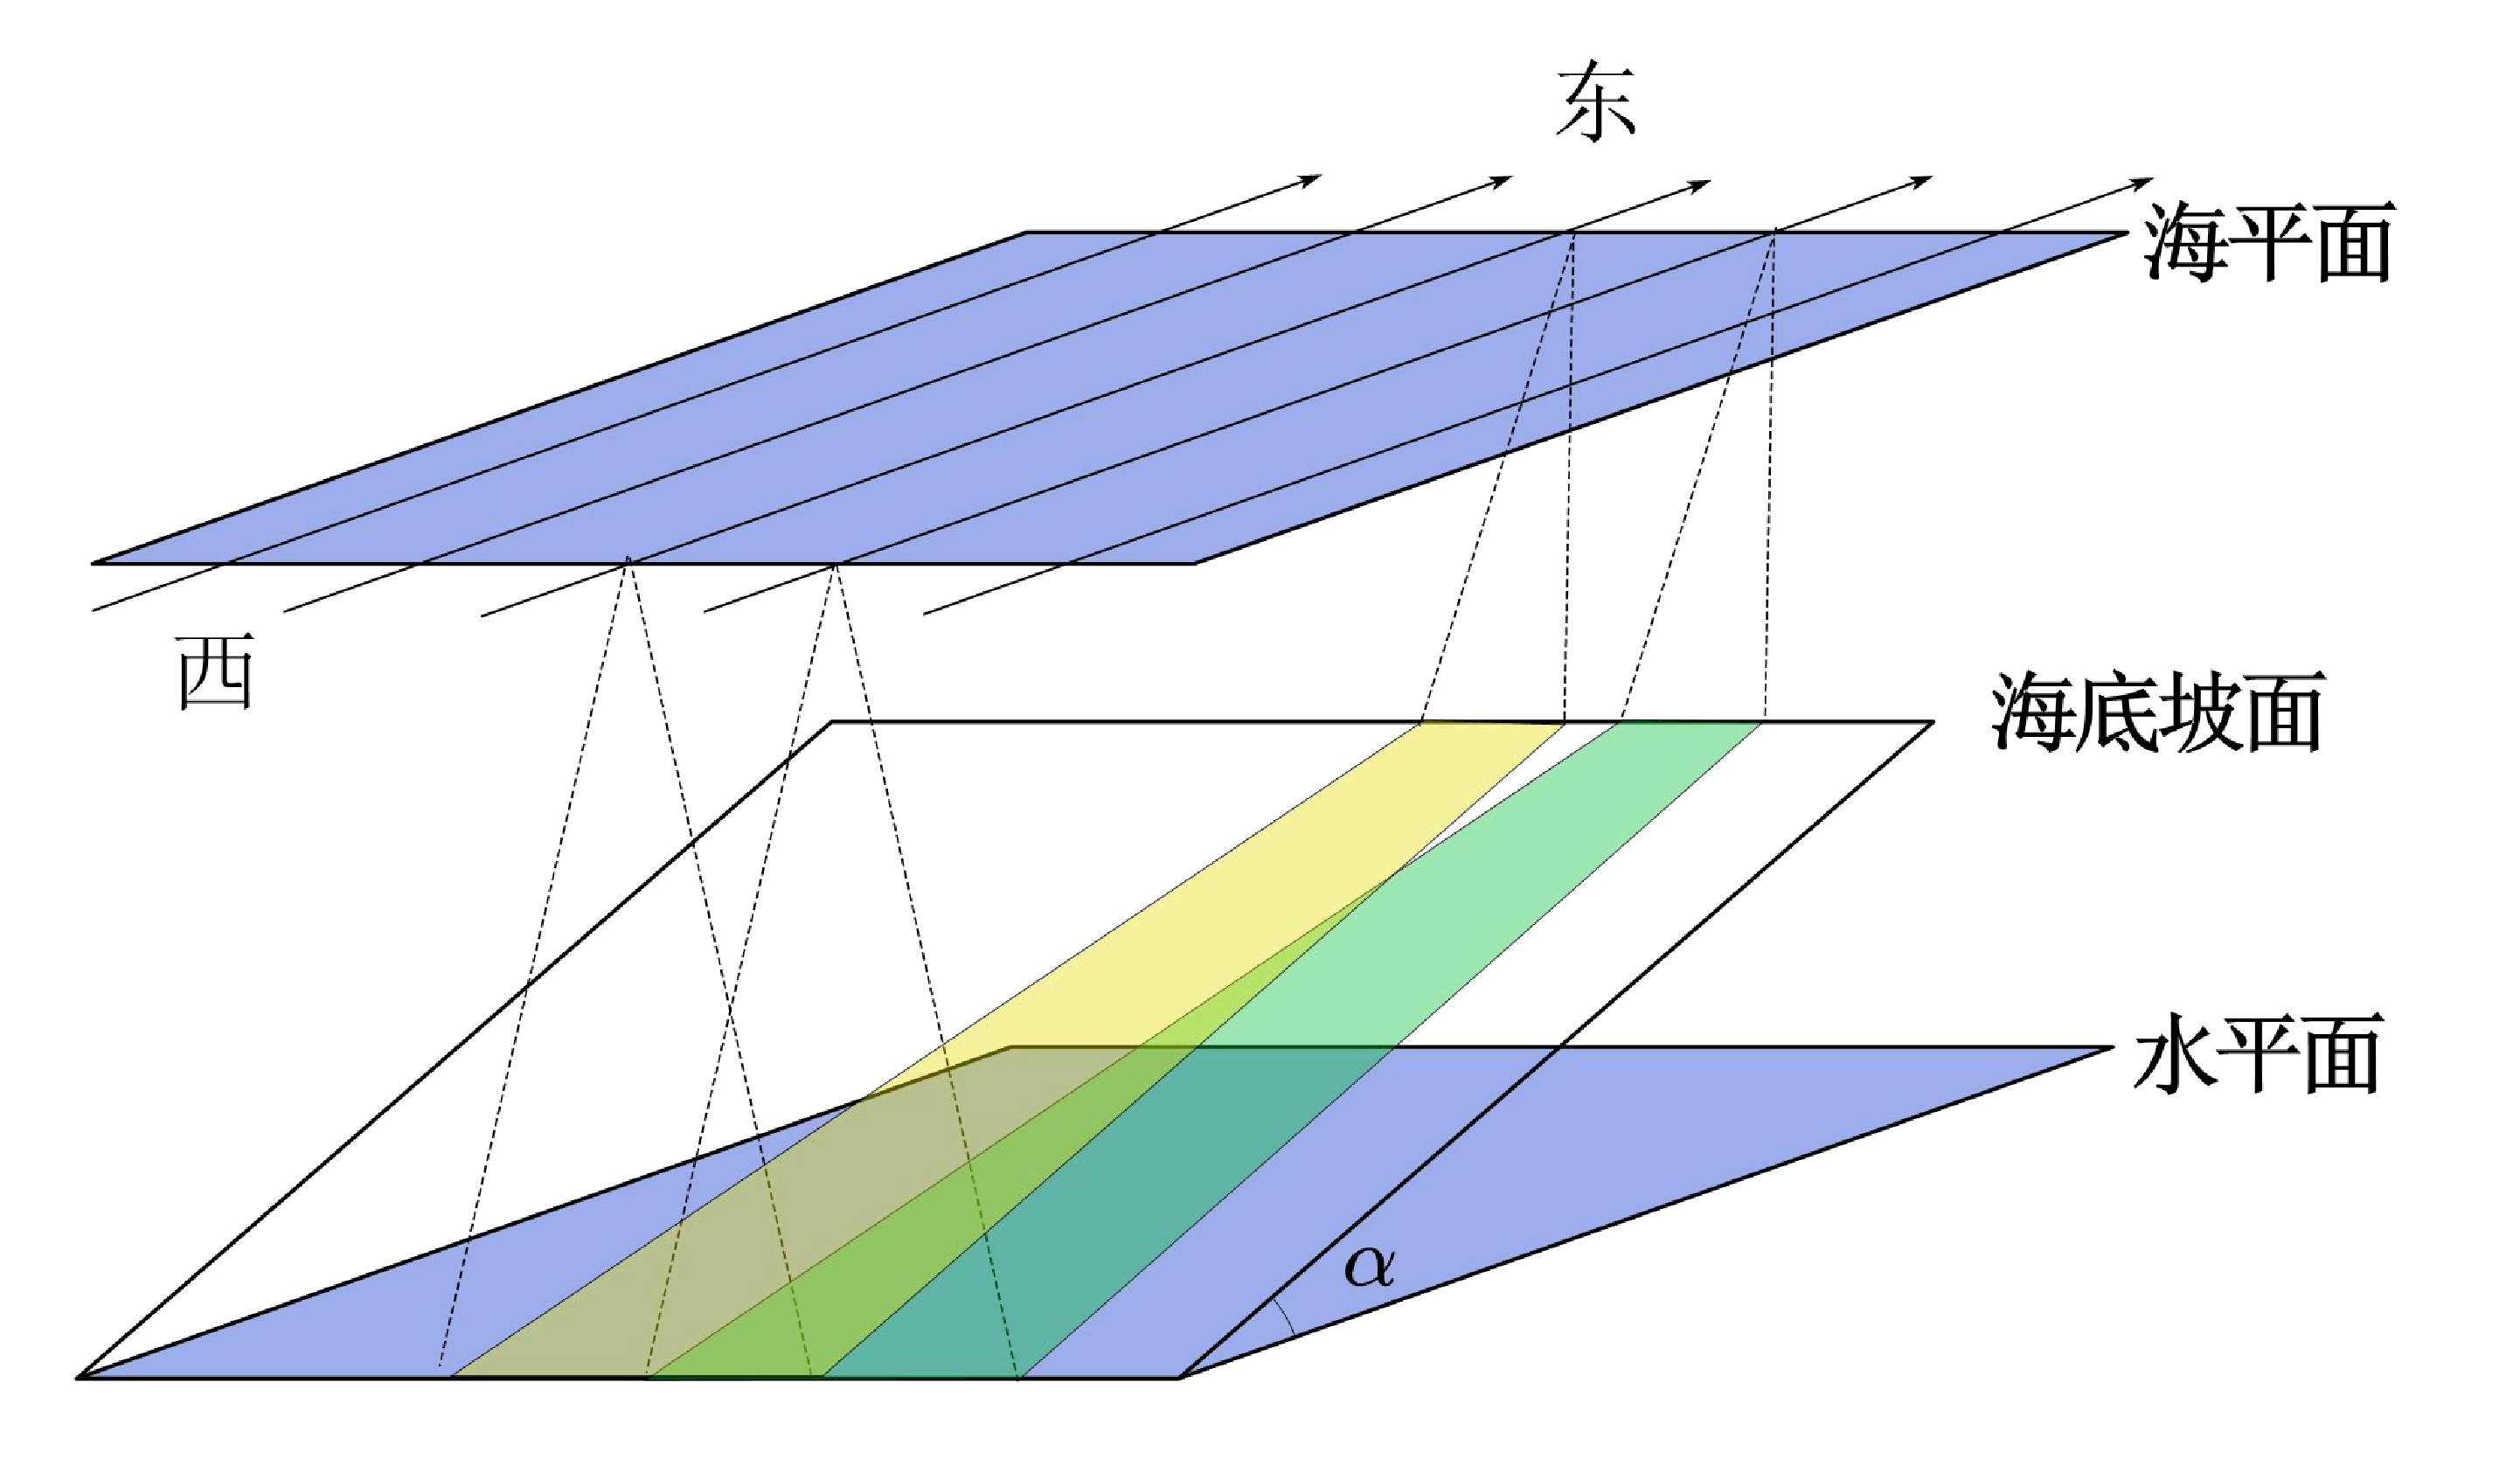
\includegraphics[width=.6\textwidth]{W_E}
            \caption{方案一示意图}
            \label{fig:W_E}
        \end{figure}
        如\cref{fig:W_E},
        此时,垂直测线方向的海床高度不变,即 $\gamma = 0$,由式\cref{eq:over_width_2}可得,此时覆盖宽度:
        \begin{equation}
            W = 2D\tan\frac{\theta}{2}
            \label{eq:over_width_3}
        \end{equation}
        可知,在固定波束张角 $\theta$ 的前提下,水深越深的区域,波束覆盖宽度越大。
        在题设海域中,测线两端(对应最深处与最浅处)水深分别为$D_{max} = 206.99m$和$D_{min} = 13.90m$,此时覆盖宽度分别为$W_{max} = 717.03m$和$W_{min} = 48.15m$。
        若希望满足不漏测的条件,则
        \begin{equation}
            d \leq W_{min} = 2D_{min}\tan\frac{\theta}{2}
            \label{range_d}
        \end{equation}
        \begin{figure}[H]
            \centering
            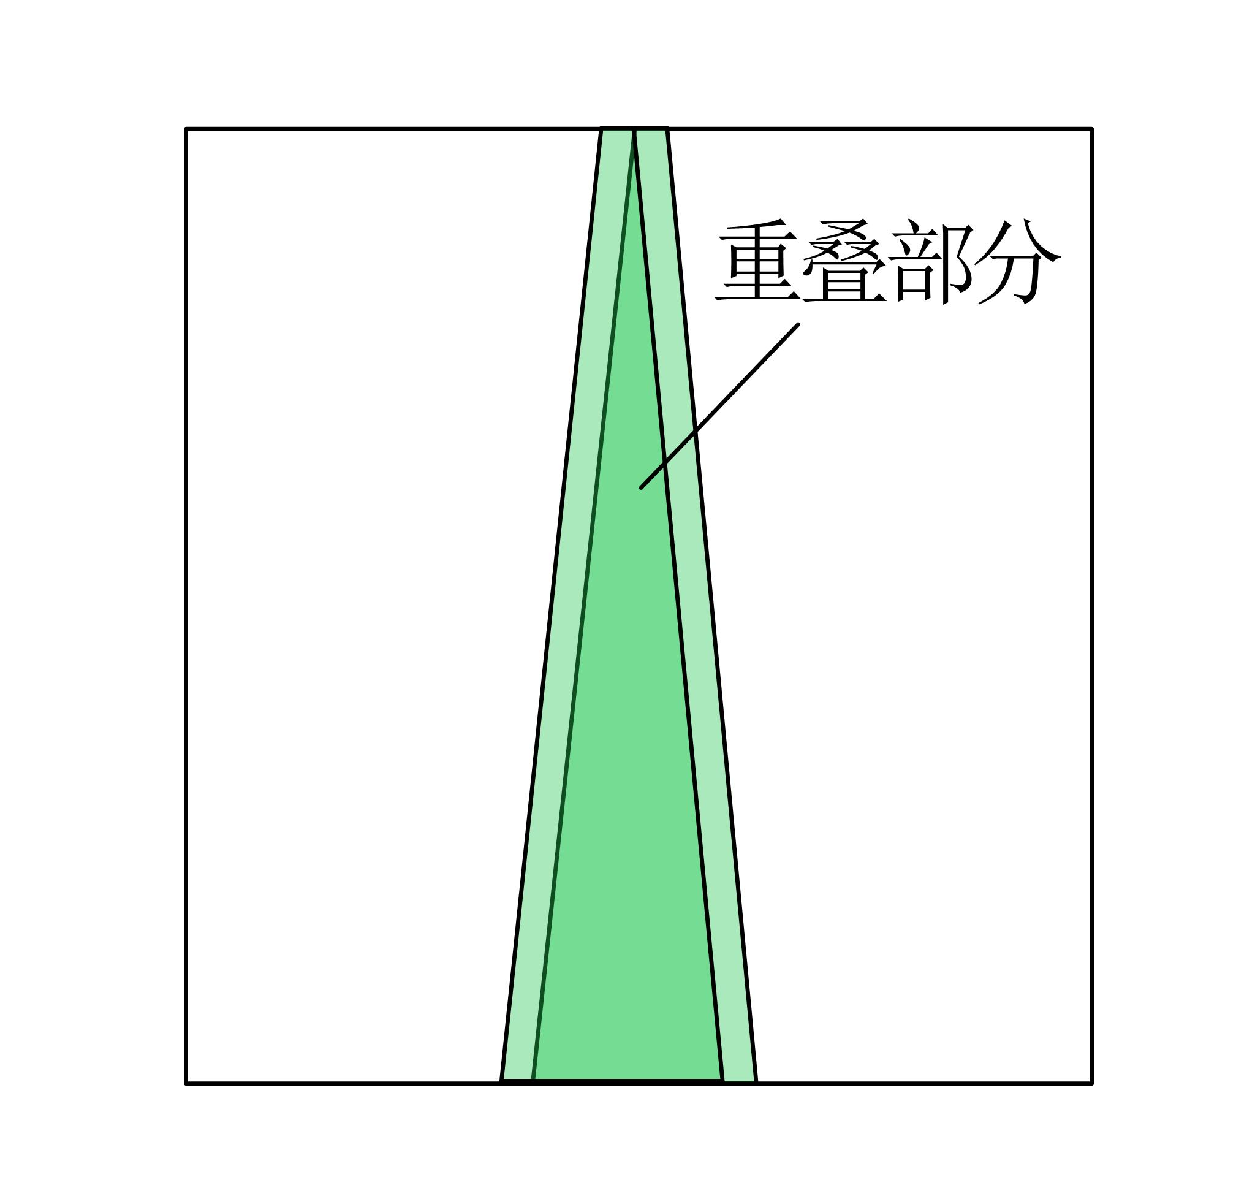
\includegraphics[width=.55\textwidth]{parallel}
            \caption{恰满足不漏测的情形}
            \label{fig:parallel}
        \end{figure}
        此时
        \begin{equation}
            \eta_S = 1 - \frac{d}{\frac{W_{min} + W_{max}}{2}} \geq 1 - \frac{W_{min}}{\frac{W_{min}+W_{max}}{2}} = 87.4\%
            \label{solve_eta_S}
        \end{equation}
        不满足条件。
        由此可知,方案一不成立。
        
        通过该方案的讨论,可得出测线设计的一个基本条件为测线两端的水深变化不应过大。
    
        \subsubsection{方案二:沿等深线方向设置测线}
        \begin{figure}[H]
            \centering
            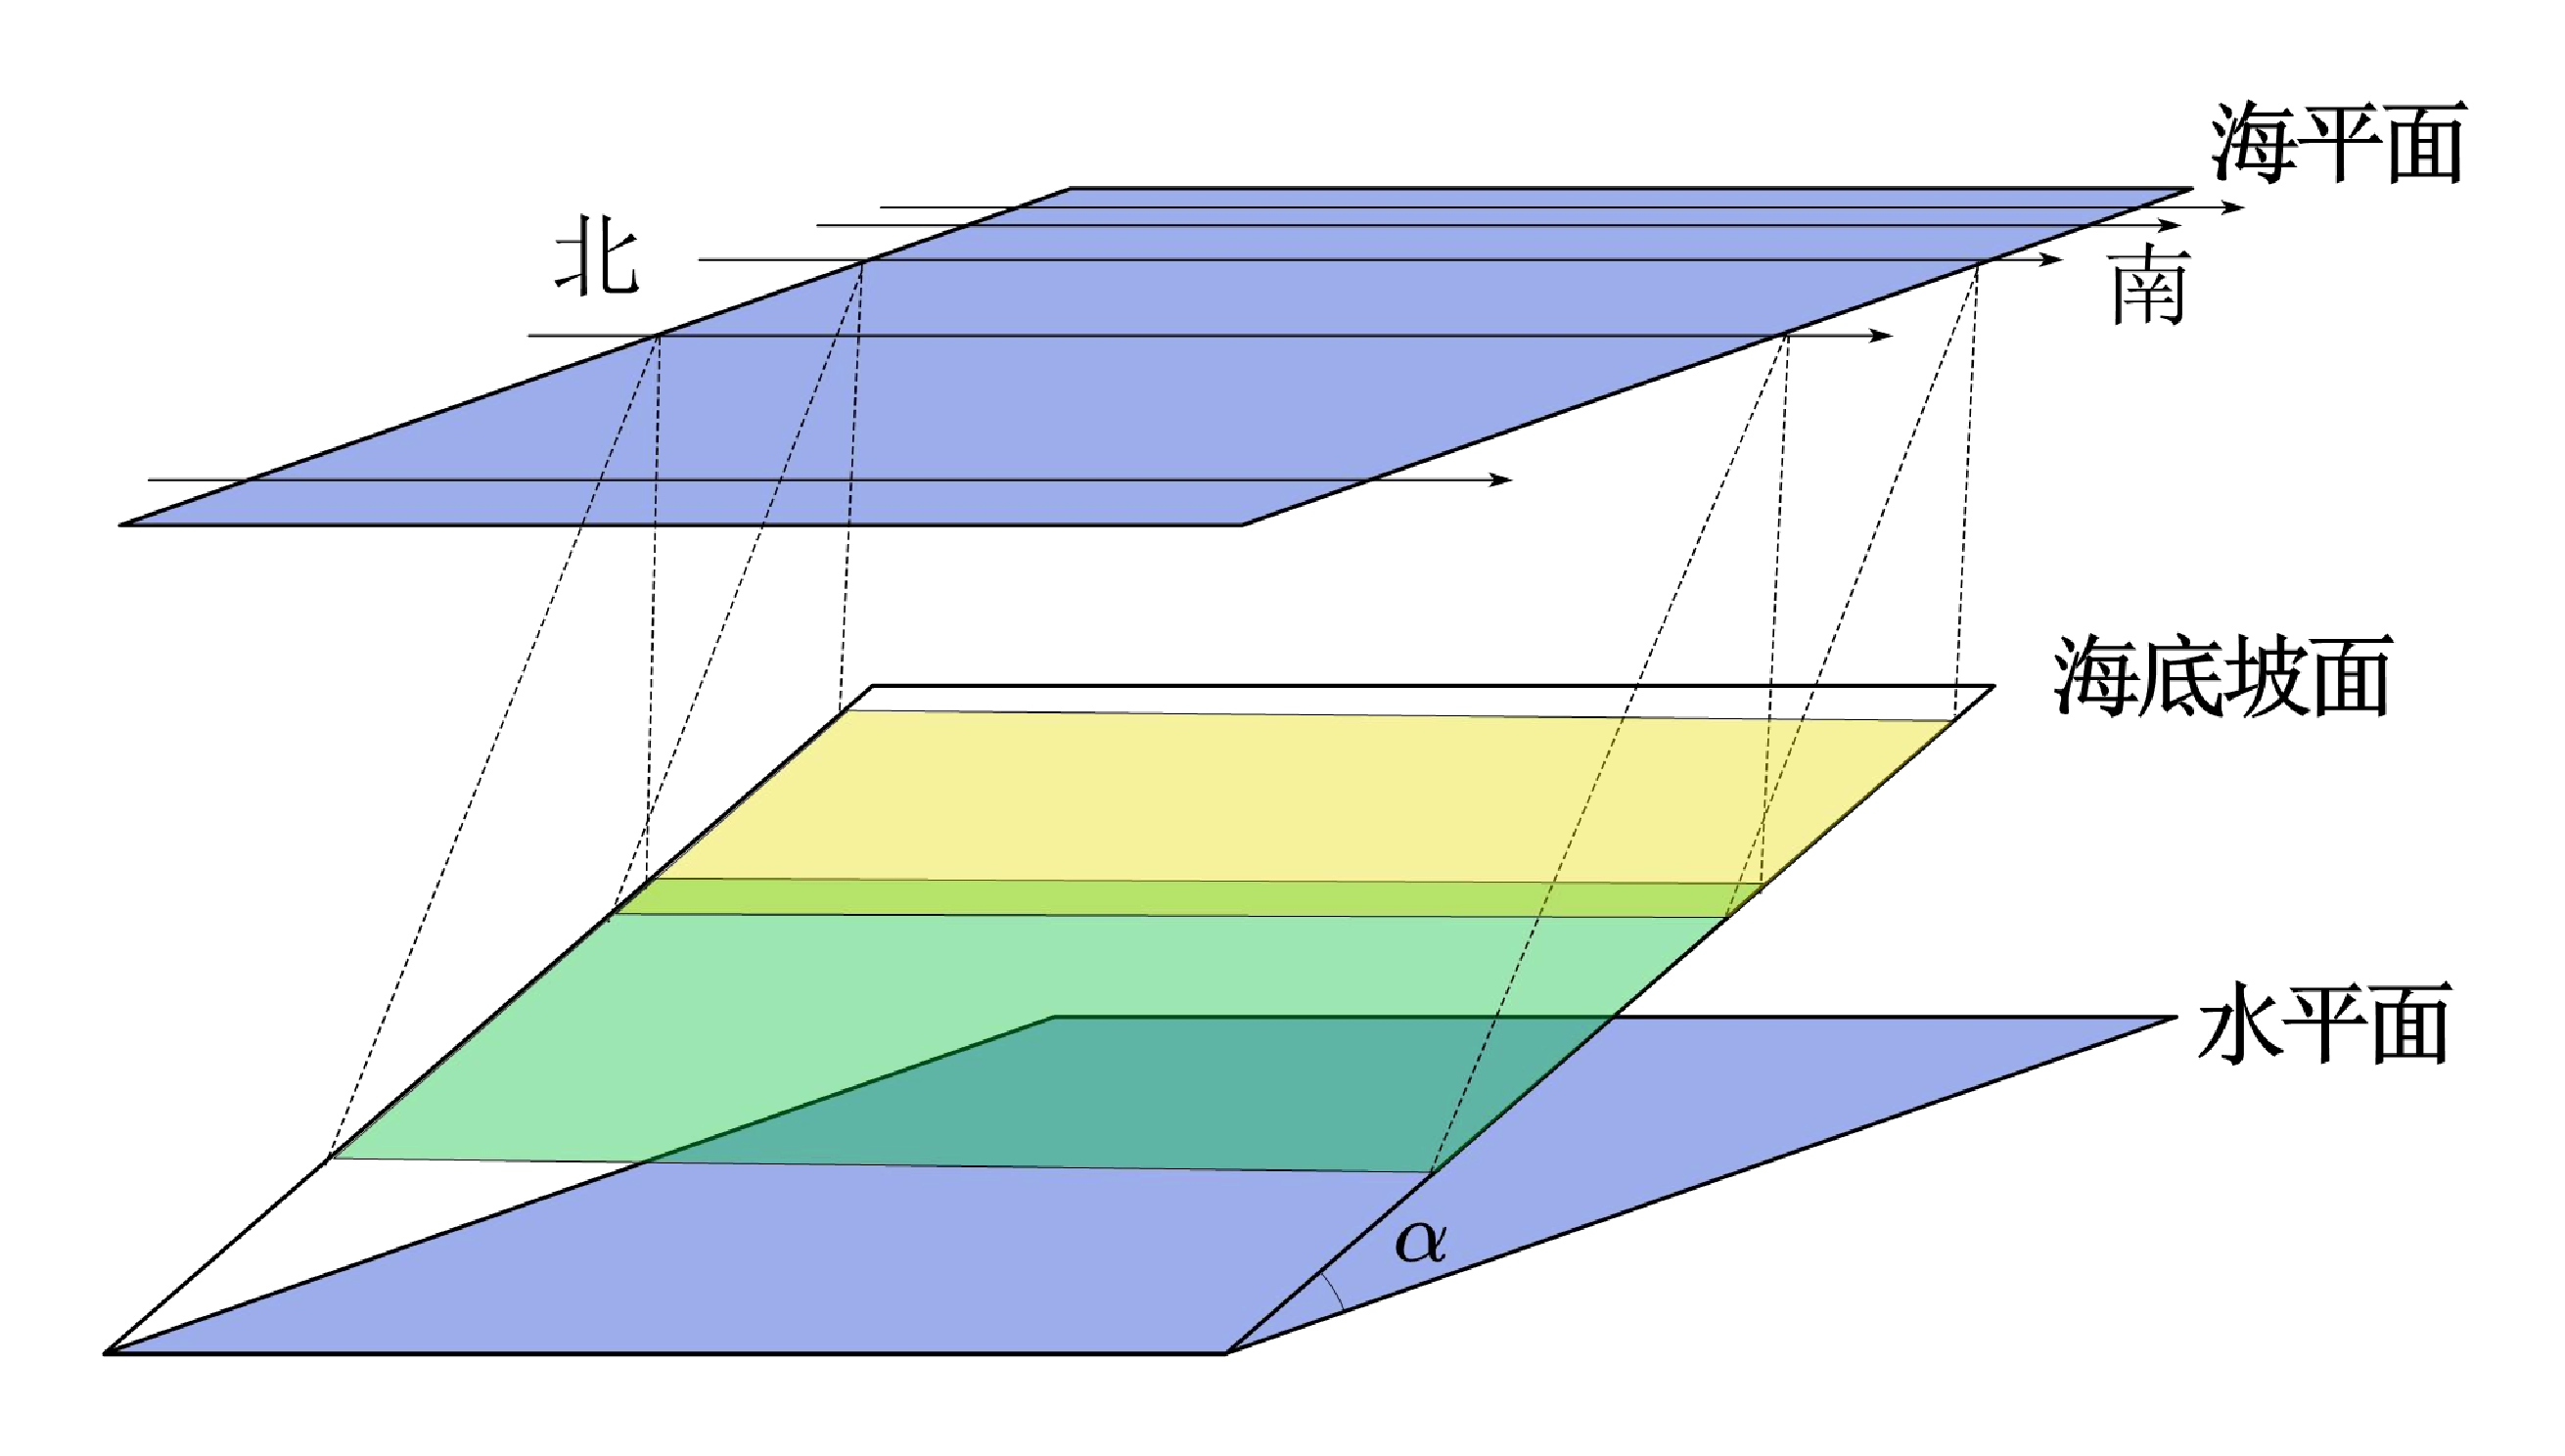
\includegraphics[width=.7\textwidth]{N_S}
            \caption{方案二示意图}
            \label{fig:N_S}
        \end{figure}
        该方案下,每条测线测量的条带形状均为矩形,由\cref{fig:N_S}可知,此时的全面积重叠率$\eta_S$与逐点重叠率$\eta$一致,均可转化为
        $\eta = \eta_S = \frac{W_r}{W}$计算。因此,可以将原问题迁移到一维的情况下求解,如\cref{fig:f5}。
        \begin{figure}[H]
            \centering
            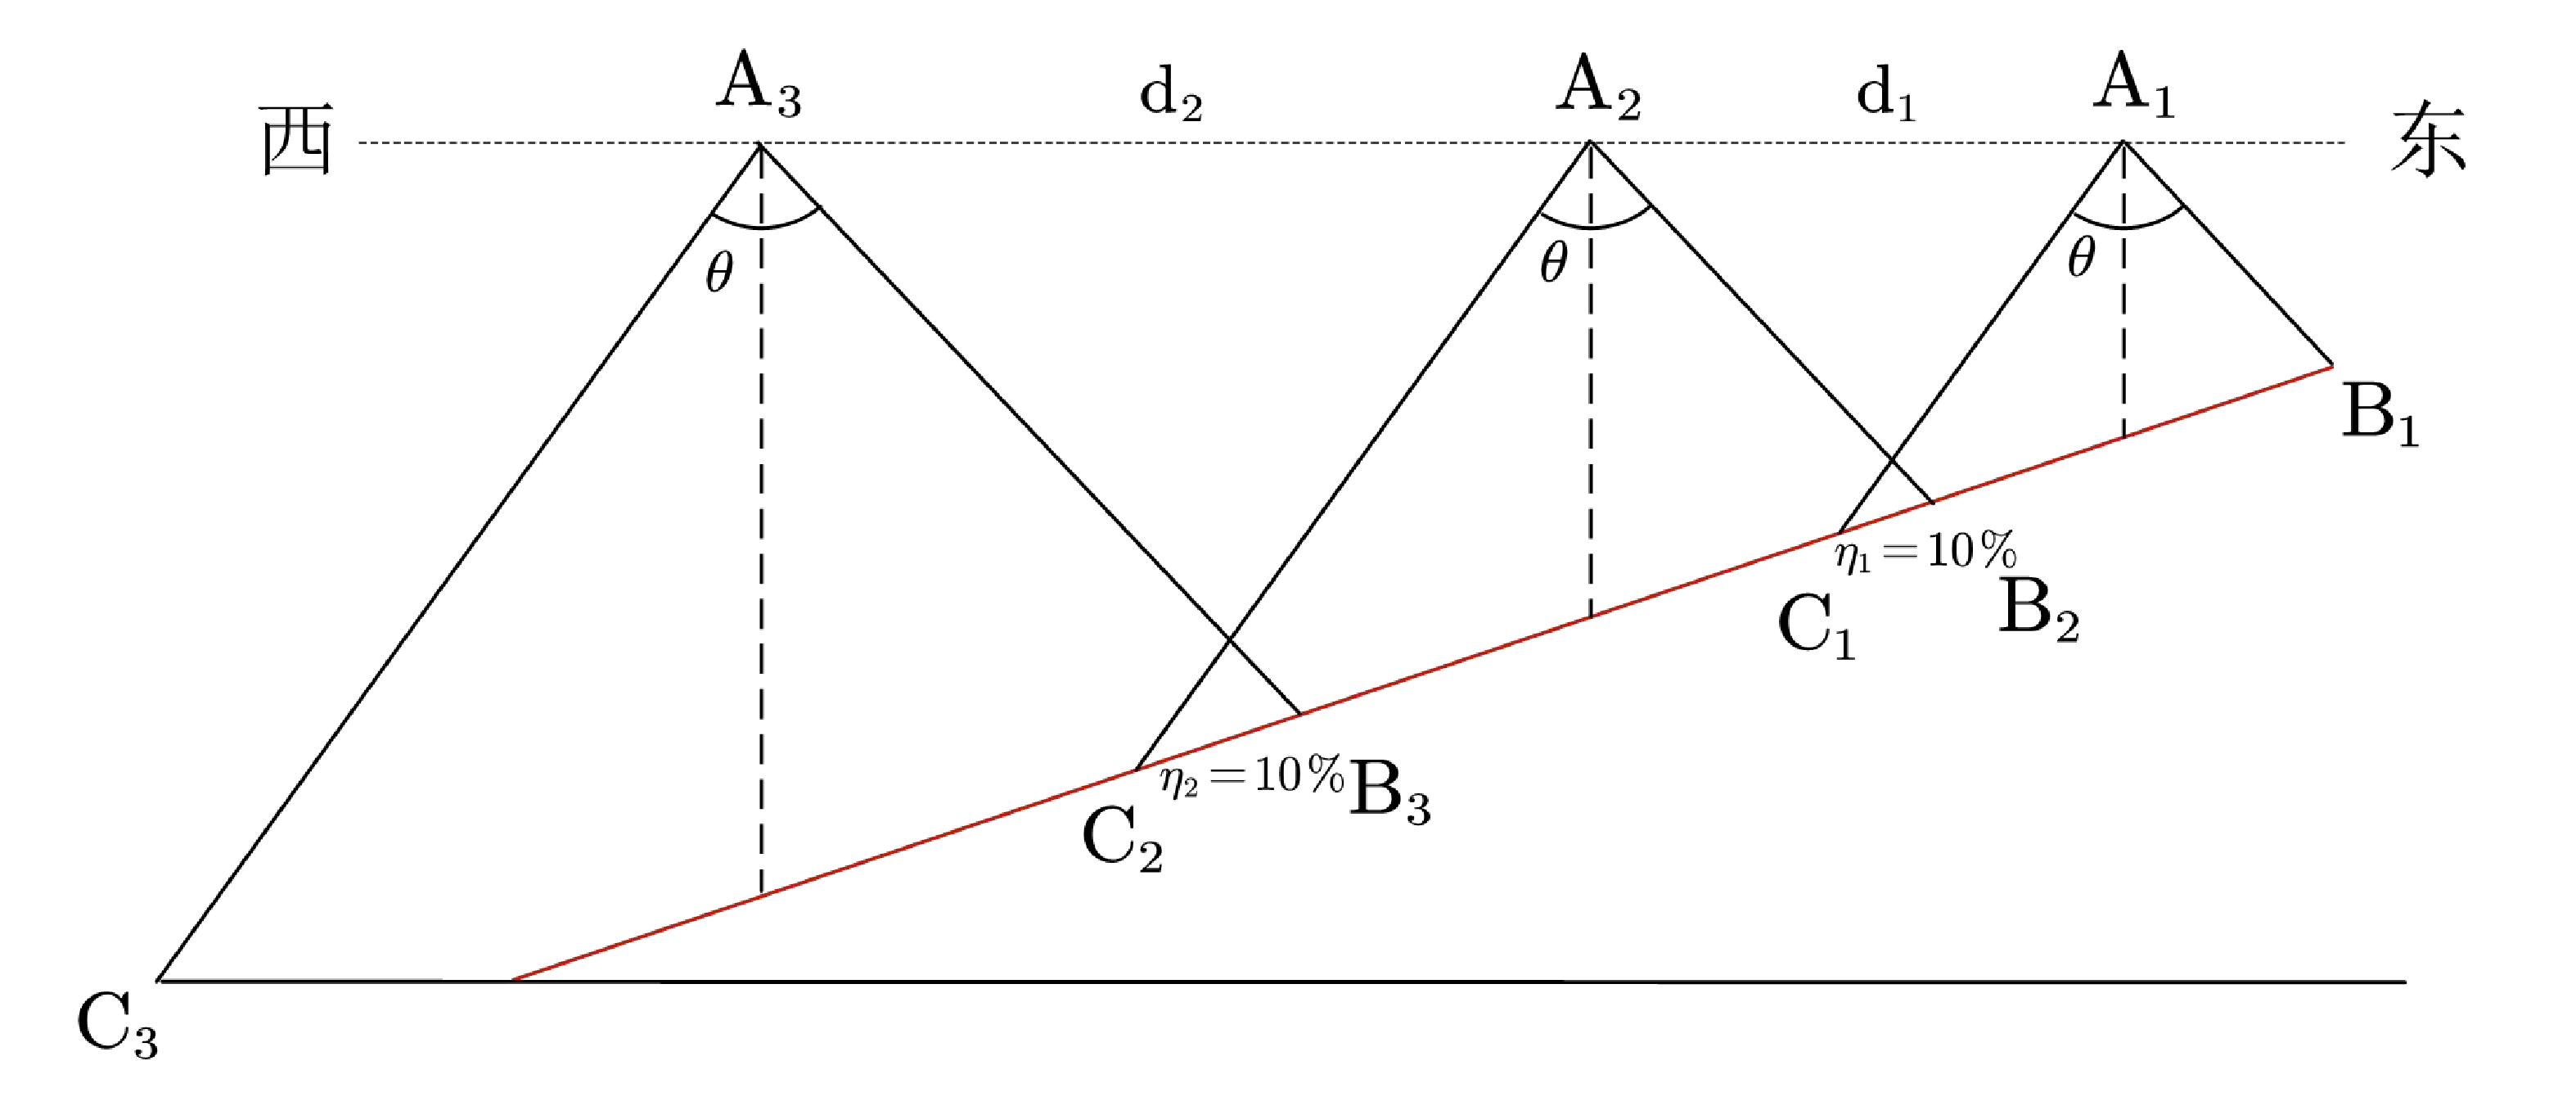
\includegraphics[width=.8\textwidth]{f5}
            \caption{贪心策略示意图}
            \label{fig:f5}
        \end{figure}
        
        同等覆盖率下,水深越深的区域测线间距越大,即测线排布沿西向东方向越来越密。

        已知优化目标为最小化总测线长度,且单条测线长度恒为$2$海里,
        因此只需最小化测线数 $n$,这可以通过求每次求得的最大化测线间距$d_i$来实现,
        故可以将问题分解为多个子问题,所以可以考虑使用\textbf{贪心算法}来求解此优化问题。
        
        贪心算法是一种寻找最优解问题的常用方法,这种方法一般将求解过程分成若干个步骤,
        并且在每个步骤选取当下最好的选择,希望以此类推堆叠出的结果也是最好的解。
        
        本文使用贪心算法来最小化测线条数,\textbf{步骤如下}:

        $\mathbf{step1}$.\textbf{从某个初始解出发}:选取恰好覆盖海域的最东侧边界的测线为第一条测线。

        $\mathbf{step2}$.\textbf{采用迭代的过程,根据局部最优策略,得到一部分解,缩小问题规模}:
        逐步求解当前测线与下一条测线的最大间距,
        在满足$\eta_1 = \frac{C_1 B_2}{C_1 B_1}$在$10\%\sim 20\%$ 的条件下,
        为让第二条测线离第一条测线尽可能远,
        令 $\eta_1 = 10\%$,
        即选取$B_2$为第二条测线的最外波束投影点,然后从该点沿
        最外侧波束方向延伸至海平面,即可求得最远的第二条测线位置与最大的$d_1$。
        以此类推,可以逐步确定所有的测线位置与所有$d_i$的最大值。
        
        $\mathbf{step3}$.\textbf{将所有解综合起来}:
        通过求得在满足约束条件下所有 $d_i$ 的最大值,进而求得了最小的测线条数 $n = 34$。
        \textbf{测线总长度的最小值}:$l_{totel} = nl = 125936.0$m。

        该方案的\textbf{最终答案}如下:
        
        \textbf{测线总长度最小值}为:$125936.0$m,
        对应的\textbf{测线间距}为:

        $\{d_i\} = \{44.41, 48.20, 52.33, 56.80, 61.66,
        66.93, 72.66, 78.87, 85.61, 92.93,
       100.88, \\109.51, 118.87, 129.04, 140.08,
       152.06, 165.06, 179.17, 194.50, 211.13,
       229.19, 248.79, \\270.06, 293.16, 318.23 , 
       345.44, 374.98, 407.05, 441.86, 479.65,
       520.67, 565.19, 613.53\}$(m)
        
        \subsubsection{方案三:与等深线呈一定角度设平行测线}
        \begin{figure}[H]
            \centering
            \includegraphics[width=.9\textwidth]{Phi}
            \caption{测线方向示意图}
            \label{fig:Phi}
        \end{figure}
        
        由方案一知,可行测线的一个必要条件是测线两端的水深变化不应过大,从而使得测线上各点的覆盖宽度 $W$ 较为一致,进而可以令测线上的所有点的逐点重叠率 $\eta$
        能同时在合理范围内,自然使全面积重叠率 $\eta_S$ 满足要求(已在问题分析中完成证明,不再赘述),且保证漏测问题与边缘波束精度较低等问题同时得到解决。
        
        
        在该方案下,每条测线的爬升率一致,均为$\tan\varphi$,则水深 $D$ 沿着测线方向均匀变化,由式\cref{eq:over_width_2}知 $W \propto D$,因此覆盖宽度 $W$ 也沿测线方向均匀增长,最终的条带形状应为梯形,且不同测线形成的梯形条带
        的两腰分别平行。由均匀增长性质,只需令测线两端点的逐点覆盖率均在$10\%\sim20\%$内,则测线上所有点的逐点覆盖率均在要求范围内。

        \begin{figure}[H]
            \centering
            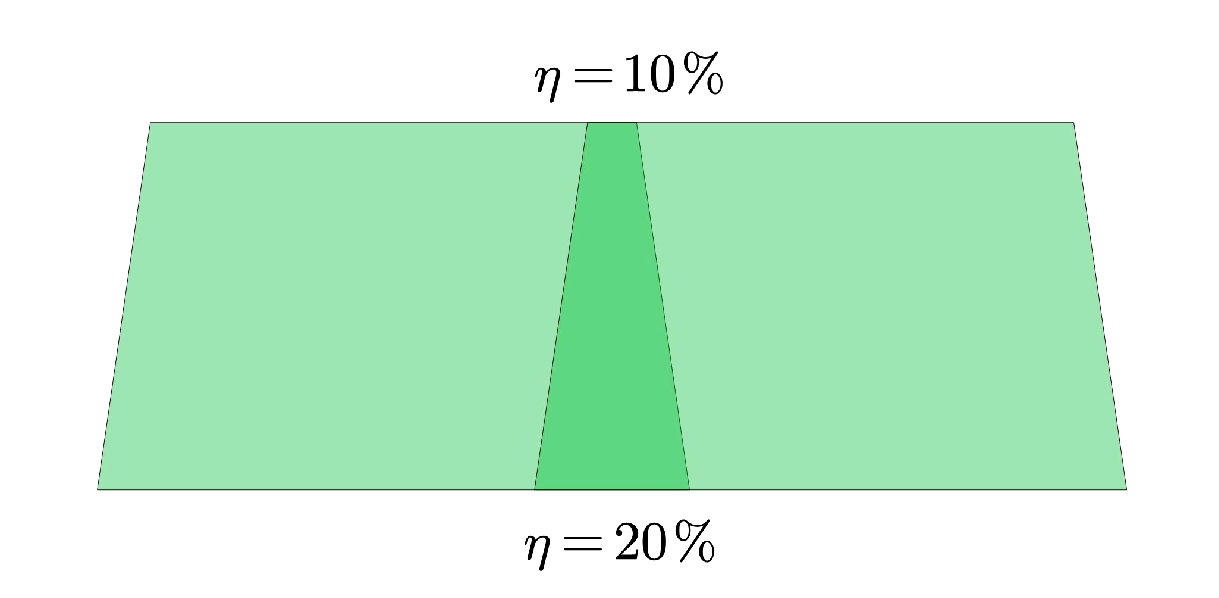
\includegraphics[width=.9\textwidth]{8_9}
            \caption{恰满足重叠率要求情形}
            \label{fig:8_9}
        \end{figure}
        如\cref{fig:8_9},考虑极端情况,让上下底重叠率分别为 $\eta = 10\%$ 和 $\eta = 20\%$, 
        可解出测线上两端点的覆盖宽度比为$\frac{9}{8}$,因此,测线上两端点的覆盖宽度比应小于$\frac{9}{8}$,即深度比应小于$\frac{9}{8}$。这要求沿测线爬升的总高度小于起点高度的$\frac{1}{8}$。由于每条测线的长度 $l$ 相等
        (除边界外),爬升率相等,因此沿测线爬升的总高度相等。因此,爬升总高度小于最小深度的$\frac{1}{8}$,即可满足要求。
        爬升高度:
        \begin{equation}
            \Delta D = l\cos\Phi\tan\alpha \leq \frac{1}{8}D_{min}
            \label{Delta_D1}
        \end{equation}
        其中,$l$ 为测线长度,可得测线与等深线的夹角$\Phi$范围为$0^\circ \sim 1.026^\circ$。
        \begin{figure}[H]
            \centering
            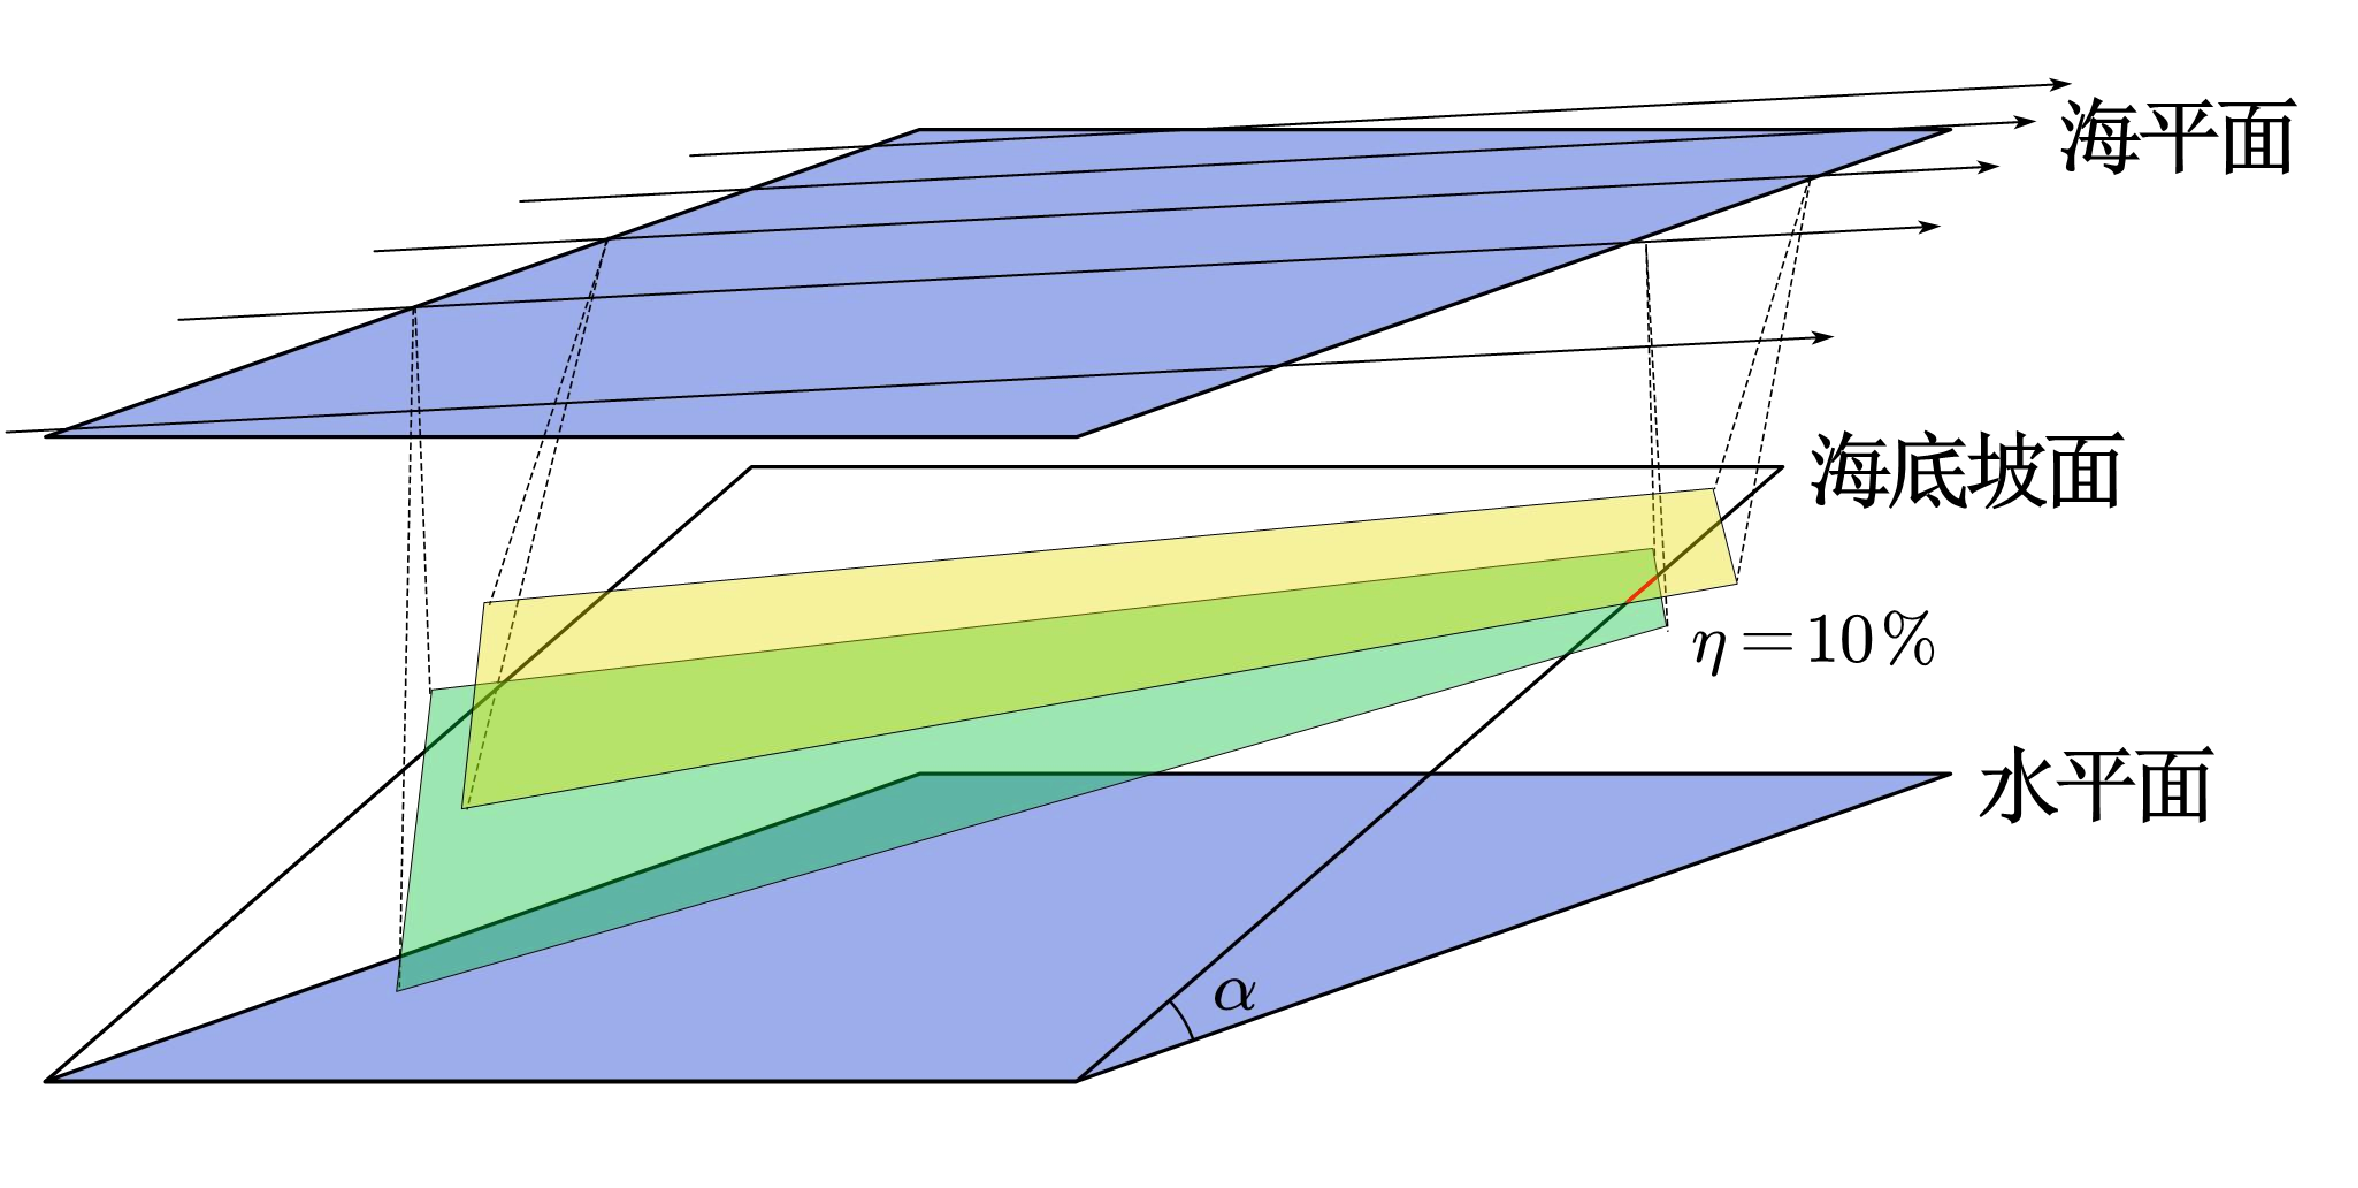
\includegraphics[width=.9\textwidth]{line}
            \caption{方案三示意图}
            \label{fig:line}
        \end{figure}
        在$0^\circ \sim 1.026^\circ$内,只需令最浅处覆盖宽度的重叠率为10\%,即可满足$d_i$最大且最深处覆盖宽度的重叠率小于20\%。
        对于每一组给定角度的测线方案,本文从最浅处入手,仍用方案二中逐步确定$d_i$的方法来确定最优间距。
        我们在$0^\circ \sim 1.026^\circ$内按$0.001^\circ$的步长进行搜索,结果如\cref{fig:result_1}。
        \begin{figure}[H]
            \centering
            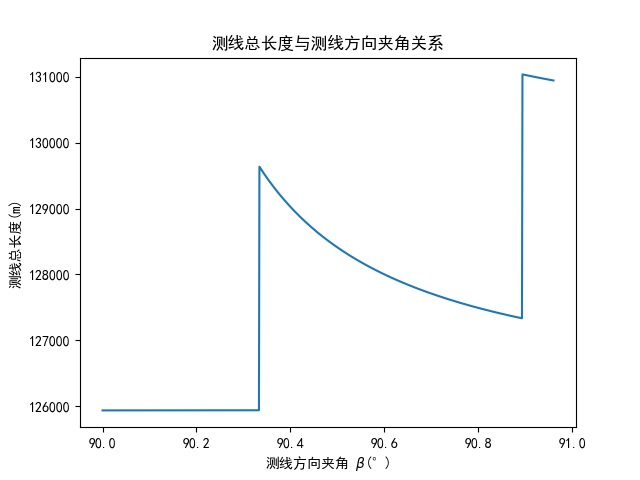
\includegraphics[width=.9\textwidth]{result_1}
            \caption{逐点重叠率条件下搜索结果}
            \label{fig:result_1}
        \end{figure}
        可知最优角度为$\Phi = 0^\circ$。
        
        若仅考虑全面积覆盖率在$10\% \sim 20\%$之间与无漏测要求,约束条件为:
        \begin{equation}
            ld \leq 0.9 l\frac{W_{max}+W_{min}}{2}
            \label{eq:condition_1}
        \end{equation}
        \begin{equation}
            d \leq W_{min}
            \label{eq:condition_2}
        \end{equation}
        为使 式\cref{eq:condition_1} 取等时 式\cref{eq:condition_2} 同时成立,即可得到:
        \begin{equation}
            W_{min} \leq 0.9 \frac{W_{max} + W_{min}}{2}
            \label{eq:target_1}
        \end{equation}
        可知最深处覆盖宽度与最浅处覆盖宽度之比小于$\frac{11}{9}$,即
        \begin{equation}
            \Delta D = l\cos\Phi\tan\alpha \leq \frac{2}{9}D_{min}
            \label{Delta_D2}
        \end{equation}
        可得测线与等深线的夹角 $\Phi$ 的范围为$0^\circ \sim 1.824^\circ$。对应确定最优$d_i$的方案如下:
        \begin{equation}
            d_i = 0.9(\frac{W_{max} + W_{min}}{2})
            \label{eq:solve_di}
        \end{equation}
        由贪心算法依次递推可得所有最优$d_i$。

        我们在$0^\circ \sim 1.824^\circ$内按$0.001^\circ$的步长进行搜索,结果如\cref{fig:result_2}。
        \begin{figure}[H]
            \centering
            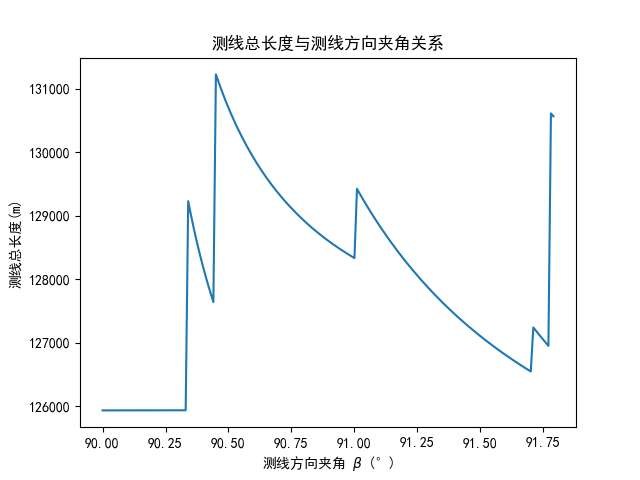
\includegraphics[width=.9\textwidth]{result_2}
            \caption{全面积重叠率条件下搜索结果}
            \label{fig:result_2}
        \end{figure}
        可知最优角度仍为 $\Phi = 0^\circ$。

        经比较可知,沿等深线设平行测线的方案总比等深线呈一定角度设平行测线的方案更优。

        \cref{fig:result_1}、\cref{fig:result_2}中突变较多,主要是因为测线条数为整数,
        而在一些边缘处出现漏测则会导致多出一条测线而导致测线总长度骤增。
        该曲线的主要控制因素为边界条件,不具有通用性。因此,在下文给出沿等深线方向设测线的方案总是最优的的普适性证明。

    
        \subsubsection{证明:沿等深线方向设测线的方案总是最优的}
        \begin{figure}[H]
            \centering
            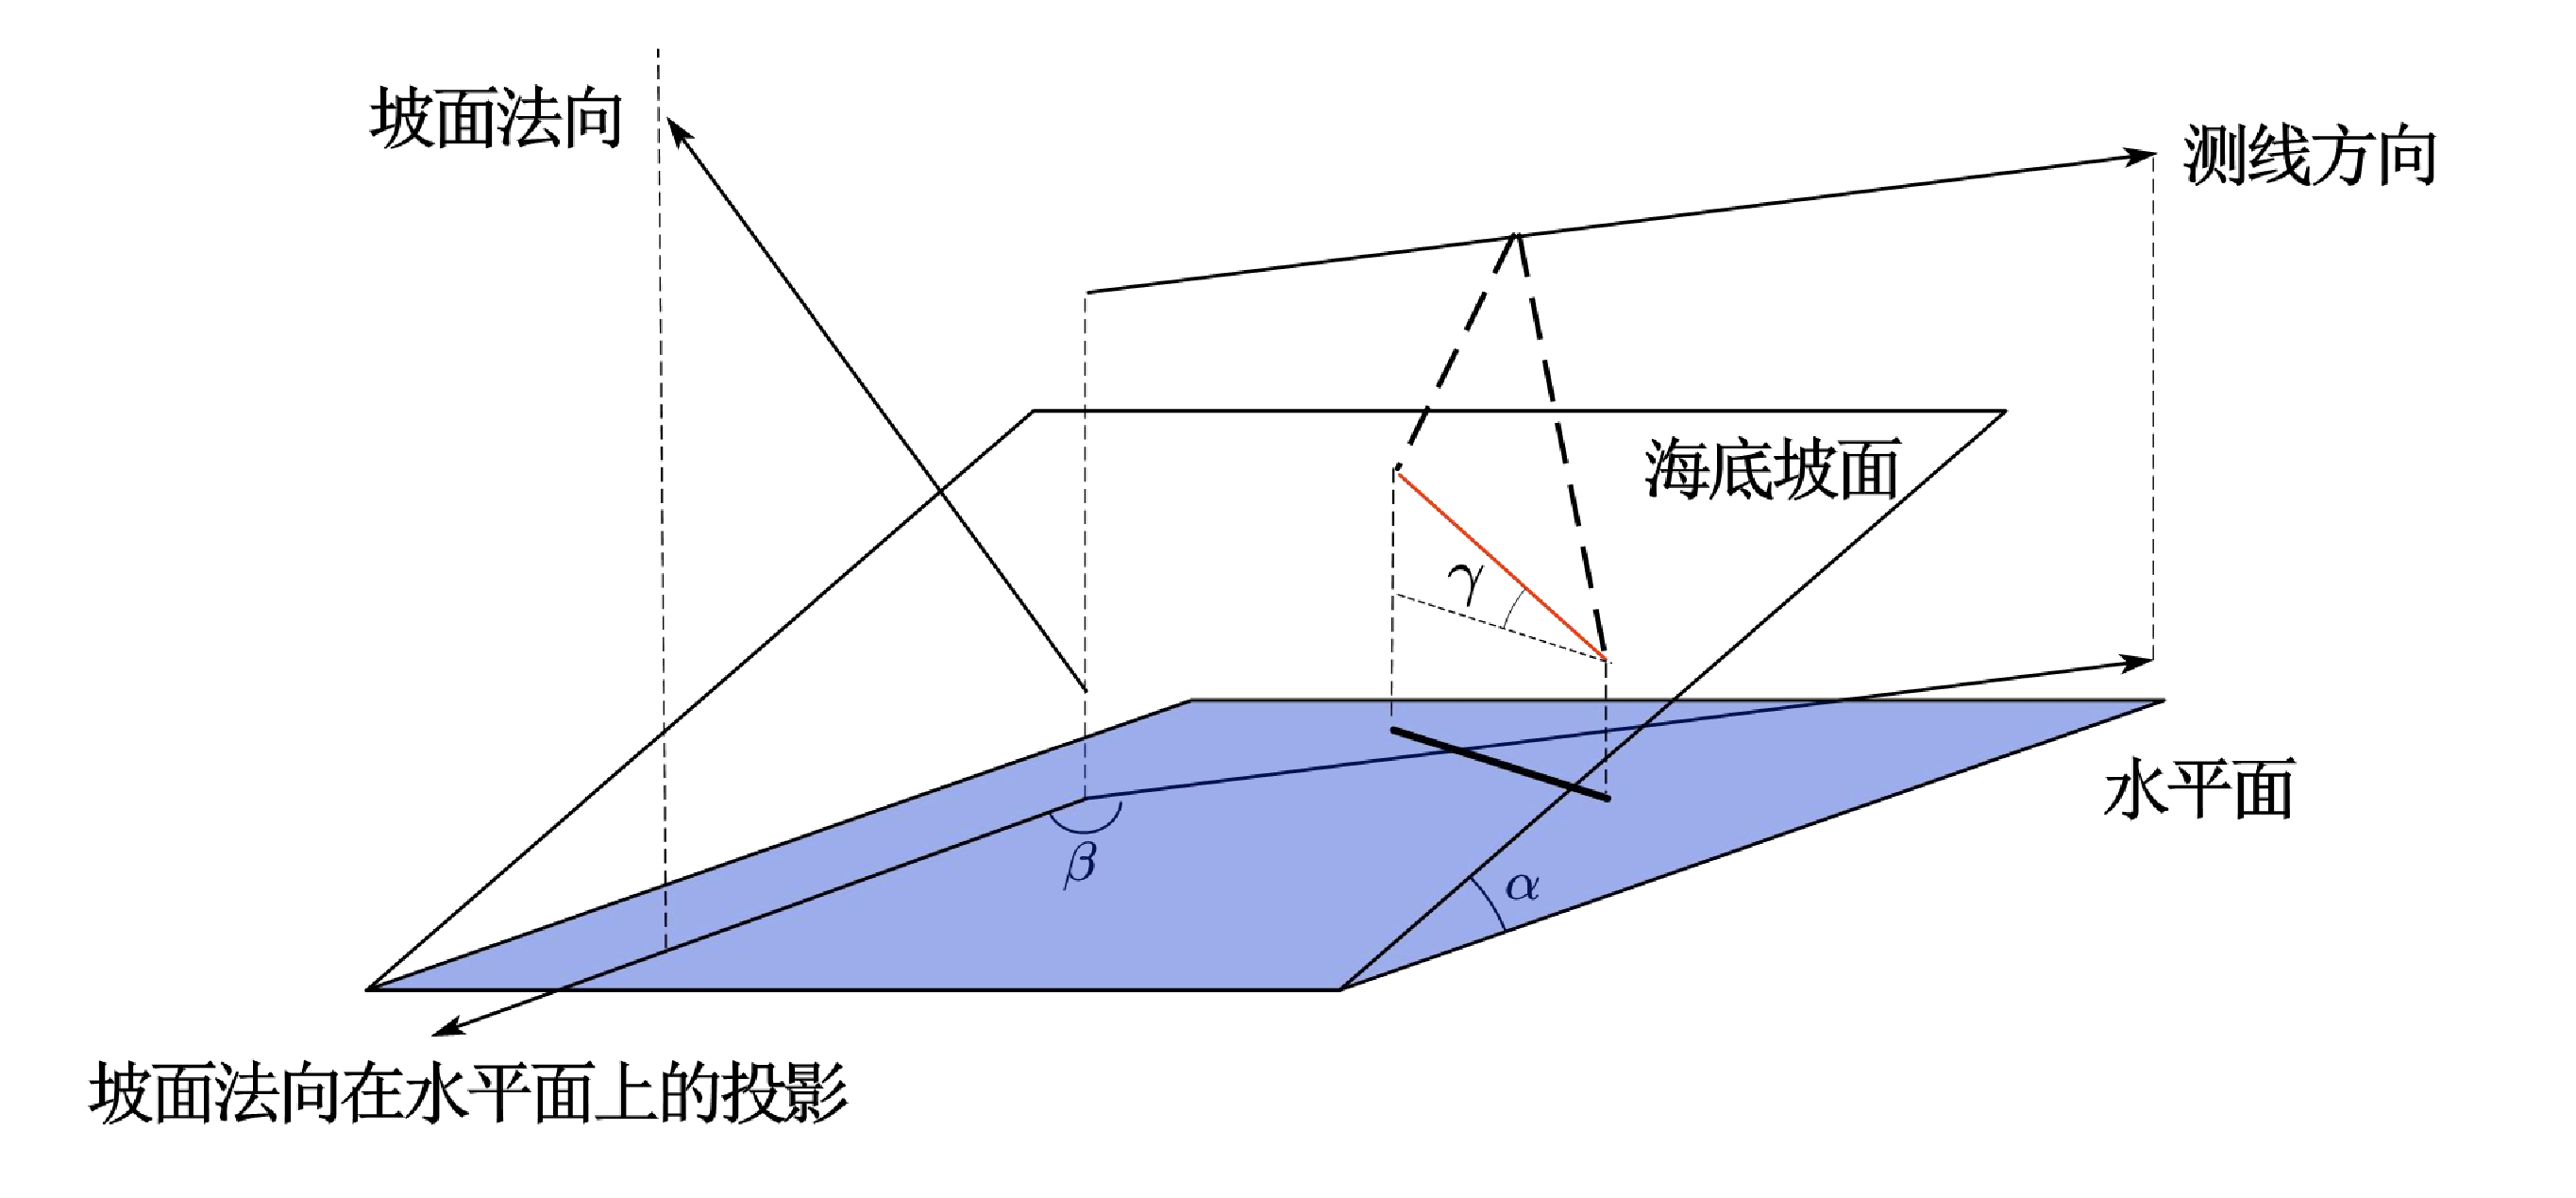
\includegraphics[width=.7\textwidth]{gamma}
            \caption{垂直测线方向爬升角示意图}
            \label{fig:gamma2}
        \end{figure}
        首先证明,在平均深度相等的情况(即测线中点重合的情况)下,沿等深线的测线的平均覆盖宽度最大。
        如\cref{fig:gamma2},当测线与等深线呈角度时,垂直测线方向(即多波束展开的方向)的爬升角为$\gamma$,由
        \begin{equation}
            \tan \gamma = \tan \alpha \cos \Phi \leq \tan \alpha
            \label{eq: solve_gamma}
        \end{equation} 
        可得
        \begin{equation}
            \gamma \leq \alpha
            \label{eq: result2}
        \end{equation} 
        又因为式\cref{eq:over_width_2}
        $$
            W = D\sin\frac{\theta}{2}(\frac{1}{\cos(\frac{\theta}{2}+\gamma)} + \frac{1}{\cos(\frac{\theta}{2} - \gamma)})\cos\gamma
        $$
        带入 $\theta = 120^\circ$ 得
        \begin{equation}
            W = 2\sqrt{3} D \frac{1}{1 - 3\tan^2 \gamma}
            \label{eq: result3}
        \end{equation} 
        显然 $W$ 随 $\gamma$ 在可行范围内单调递增。可知当覆盖宽度 $W$ 达到最大,即 $\gamma = \alpha$ 时,$\Phi = 0^\circ$,即在测线平均深度相等的情况下,沿等深线的测线的平均覆盖宽度最大。
        
        在重叠率要求相同的情况下,由
        \begin{equation}
            S = \int_{0}^l Wdl
            \label{eq: S}
        \end{equation} 
        可得测线平均覆盖宽度越大,条带面积
        等长的测线形成的条带面积越大。在同等覆盖率要求下,可行的测线间距越大。

        再考虑到每条与等深线呈角度的测线的长度为$\frac{2}{\cos\Phi}$(海里),比沿等深线角度测线更长。且为保证条带覆盖到边角处,前者需要加入补漏测线而使总测线长度
        再次变长。

        非平行测线方案中必然存在大量与等深线呈角度的测线,故也必然劣于沿等深线设平行测线的方案。
        
        

        \subsubsection{最终求解结果}
        
        综上可知,布设测线的最优方案为\textbf{沿等深线平行排布},并随深度情况适应间距。
        \textbf{测线总长度最小值}为:$125936.0m$,
        对应的\textbf{测线间距}为:

        $\{d_i\} = \{44.41, 48.20, 52.33, 56.80, 61.66,
        66.93, 72.66, 78.87, 85.61, 92.93,
       100.88, 109.51, \\118.87, 129.04, 140.08,
       152.06, 165.06, 179.17, 194.50, 211.13,
       229.19, 248.79, 270.06, 293.16, 318.23 , \\
       345.44, 374.98, 407.05, 441.86, 479.65,
       520.67, 565.19, 613.53\}$(m)
        \subsection{问题四模型的建立与求解}
        关于优化目标的转化与确定已在问题分析中讨论,此处不再赘述。本文分五个步骤求解问题四:
        (1)分析波束开角、海深数据等不需调整的数据;(2)求解条带面积的近似计算公式;(3)求解相邻波束的重叠率、总漏测率等指标的计算方法;(4)设计测线最优布线方案;
        (5)根据海底地形特征对原有方案进一步优化。
        \begin{figure}[H]
            \centering
            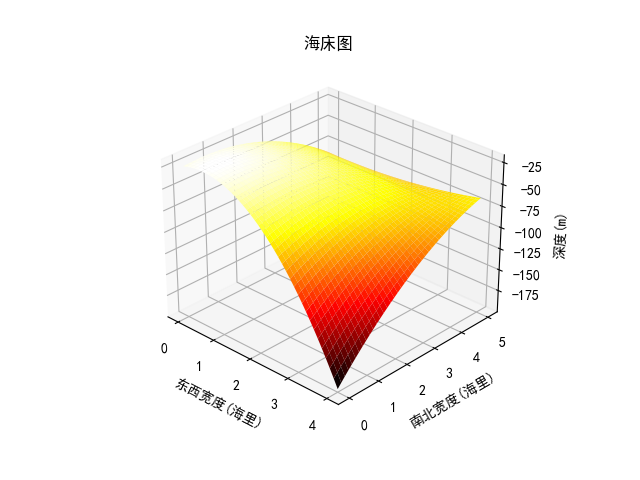
\includegraphics[width=.8\textwidth]{3D_sea_bed}
            \caption{$3D$海底地形图}
            \label{fig:3D_sea_bed}
        \end{figure}
        \subsubsection{模型准备:多波束换能器开角的确定}
        问题四中未限制波束的开角 $\theta $,故需要根据实际情况先确定一个合理的开角。通过查阅文献\cite{bib_4},发现开角 $\theta$ 不能无限接近$180^\circ$的原因有二:
        1. 边缘波束的精度较低,过大的开角会导致大量数据因精度过低而不可用。
        2. 多波束测深得到的误差方差满足$\sigma^2 \approx [D(1-\cos \frac{\theta}{2})]^2$的关系,当开角接近$180^\circ$时,误差方差接近$120^\circ$时的四倍。

        由此可知,开角应尽可能大,但有一个上界。通过查阅文献\cite{bib_2},发现实际测量中一般要求覆盖宽度为海深的$2\sim 4$倍,即对应开角$\theta$范围$90^\circ \sim 126.87^\circ$。
        为方便计算,仍取$120^\circ$作为换能器的开角。
        \subsubsection{模型准备:海深分布数据的分析}
        由问题分析四可知,题中所给单波束测量数据事实上已经过预处理,且分辨率较为合理,故不再对深度数据本身做插值处理。

        将题设数据可视化,将不同范围内的深度映射为不同颜色,并画出每 $10$ 米的等深线用于辅助分析。
        \begin{figure}[H]
            \centering
            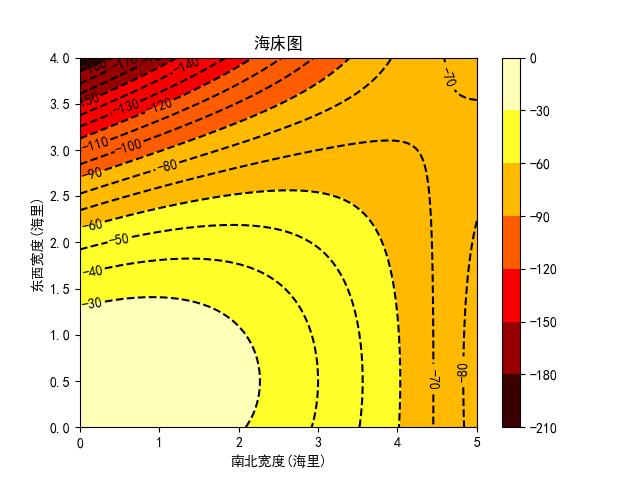
\includegraphics[width=.9\textwidth]{sea_bed}
            \caption{海底等深线图}
            \label{fig:sea_bed}
        \end{figure}
        由\cref{fig:sea_bed}可见,图中的等深线疏密程度不一,延伸方向不一,不同区域的深度也有较大差异。由问题三的分析可知,测线应尽可能平行于等深线,且应该在浅海区密集分布,深海区
        稀疏分布。因此,可将海域根据深度分布剖分为多个区域,再进行分析,后文给出一种具体的海域划分。

        \subsubsection{模型准备:测线条带近似计算方法}
        \begin{figure}[H]
            \centering
            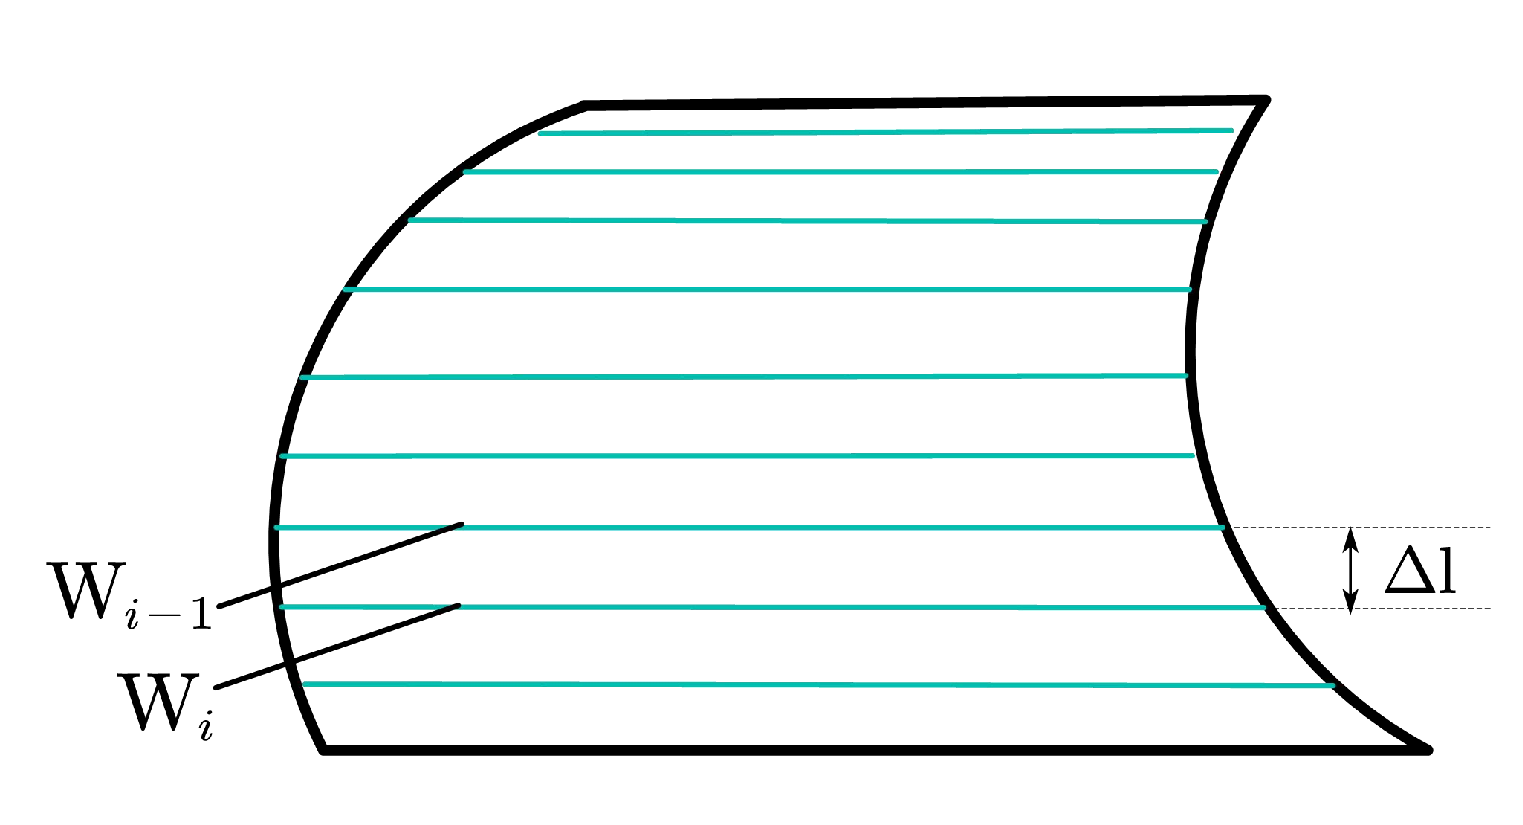
\includegraphics[width=.6\textwidth]{int}
            \caption{测线条带面积近似计算方法}
            \label{fig:int}
        \end{figure}
        题目要求对方案的相邻条带重叠率,测量覆盖率进行测量,因此必须先给出从测线到条带的计算模型。
        若认为海面是连续的,则条带应为一个曲边梯形。考虑到深度数据是离散的,本文给出的条带模型也是离散的,如\cref{fig:int},即只给出沿测线方向所有检查点的覆盖宽度,
        并根据
        \begin{equation}
            S = \sum\limits_{i=1}^{n} \frac{W_i + W_{i-1}}{2} \Delta l
            \label{eq: cross_point}
        \end{equation}
        进行\textbf{数值积分}来计算出总覆盖面积。

        计算覆盖宽度的原始方法为投影法,即直接计算两条最外侧波束与海底面的交点。
        设海底面可表达为$f(x, y, z) = 0$,最外侧波束方向向量为$(\Delta x, \Delta y, \Delta z) $,
        则交点方程为:
        \begin{equation}
            f(x + t \Delta x, y + t \Delta y, z + t \Delta z) = 0
            \label{eq:cross_point}
        \end{equation}  
        又因为数据是离散的,上式可能恒不成立,故将上式弱化为:
        \begin{equation}
            arg\min_{t} f(x + t \Delta x, y + t \Delta y, z + t \Delta z)
            \label{eq:target_3}
        \end{equation} 
        其几何意义为
        选取最外侧波束对应射线上最接近海底平面的点。

        考虑到点的数量较多,投影法计算量过大,本文提出了一种覆盖宽度的近似计算方法:用当前点正下方的海底视为局部平面,用沿垂直测线方向两侧延伸一定距离(一般取为水深的 $1.5$ 倍)取得的点的深度差除以两点间距离近似为附近区域的爬升率,
        沿用问题二中式\cref{eq:over_width_2}直接给出当前点下方的覆盖宽度的估计值 $\hat{W}$,并给出左右边界点在海面上的投影坐标,如\cref{fig:pr_W}:
        \begin{figure}[H]
            \centering
            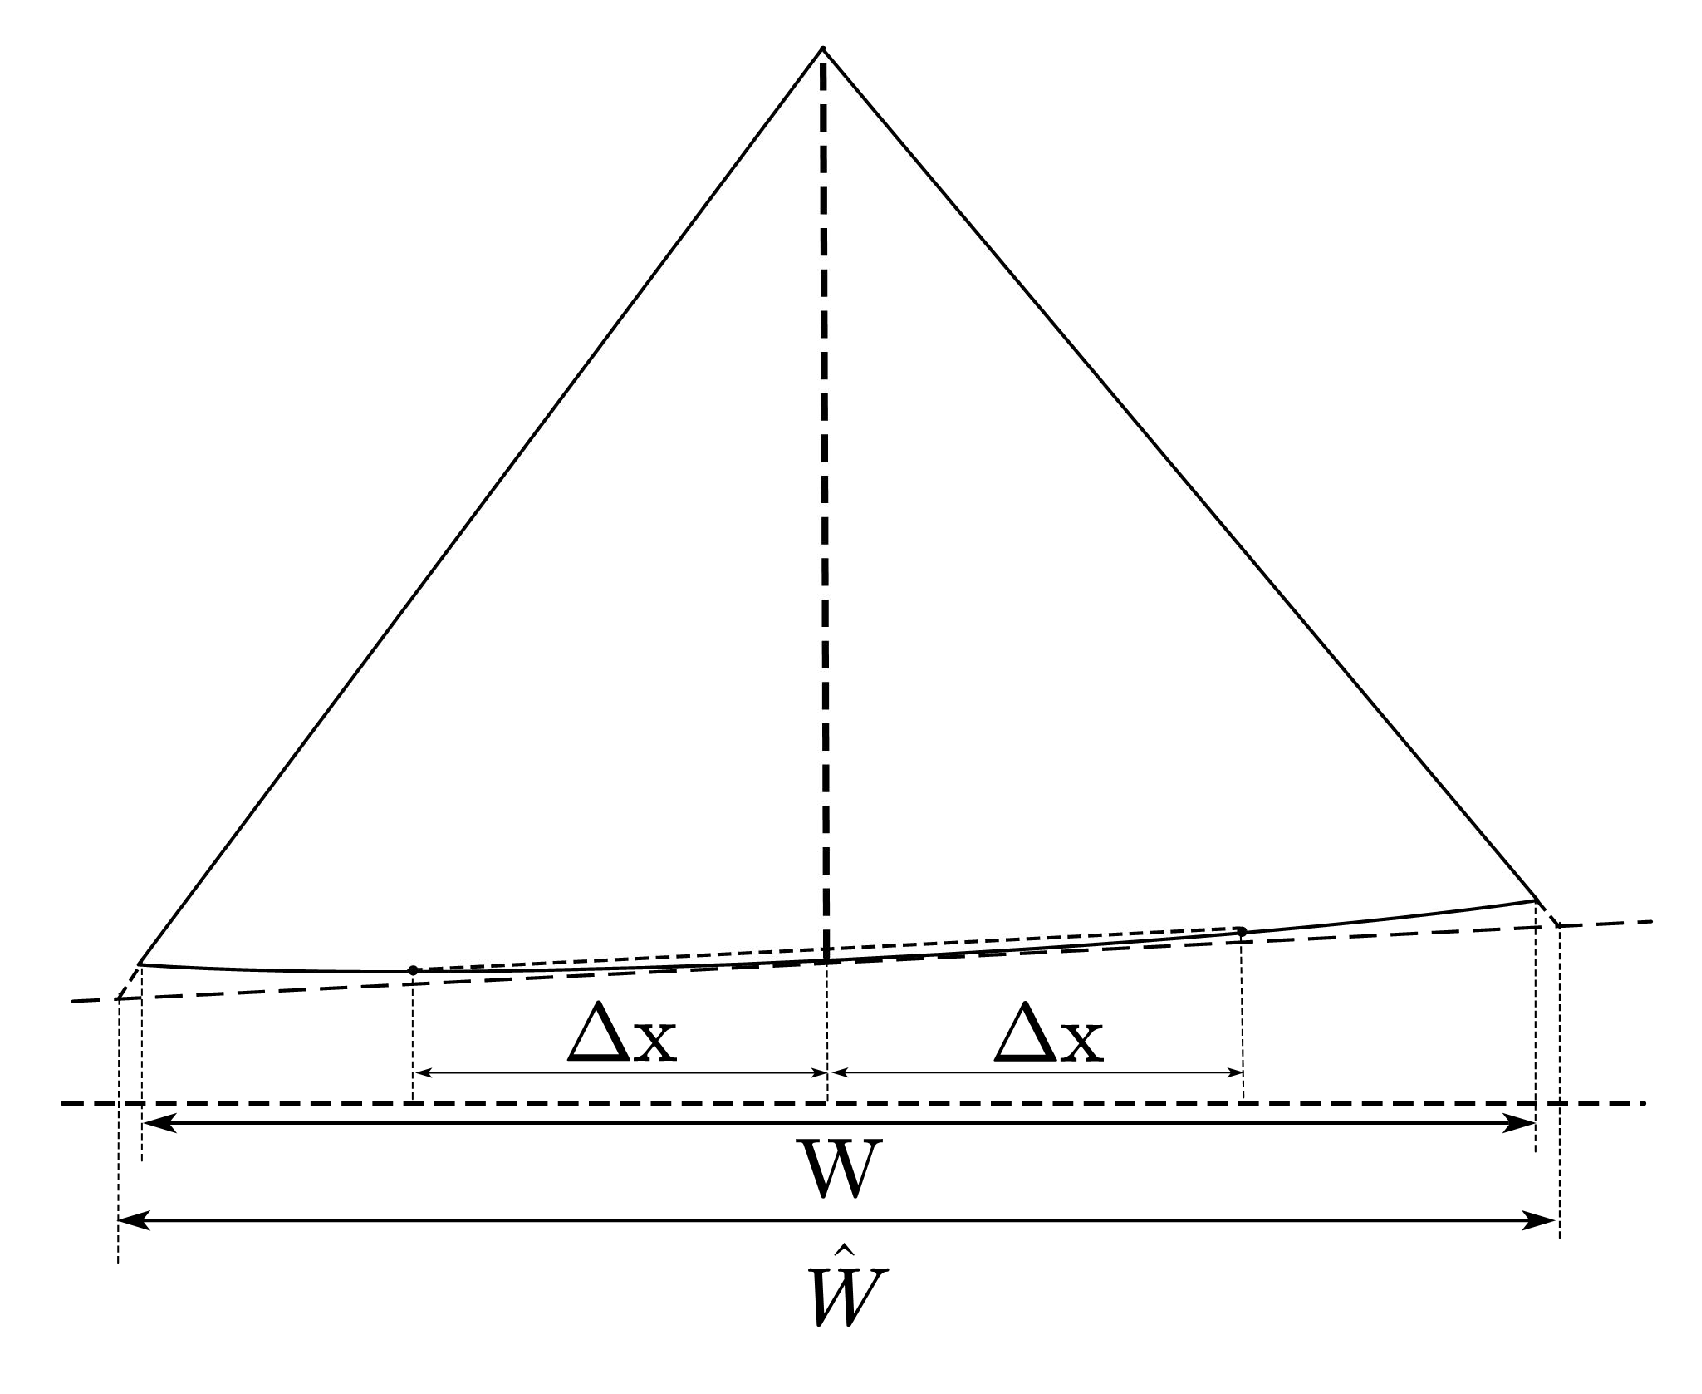
\includegraphics[width=.45\textwidth]{pr_W}
            \caption{覆盖宽度的一种近似算法}
            \label{fig:pr_W}
        \end{figure}

        \subsubsection{模型准备:相邻条带重叠率计算方法}
        先考虑两条相邻平行测线的条带重叠率。由于条带模型是离散的,可将条带重叠率 $\eta_S$(全面积意义)转化为两条测线上对应检查点的覆盖宽度重叠率 $\eta$ 的加权平均值(权重为覆盖宽度$W$),
        即
        \begin{equation}
            \eta_S =\frac{S_r}{S} = \frac{\sum\limits_{i=1}^n W_i\eta_i}{\sum\limits_{i=1}^n W_i}
            \label{eq:eta_S}
        \end{equation}
        考虑到两条相邻平行测线的长度可能有差异,检查点数量可能不同,故在计算前应先将两条测线上的检查点进行匹配,具体流程如下:
        取测线倾斜方向外侧的测线的起始点作为该测线的第一个检查点,然后找到另一条测线上与该点最接近的检查点作为另一条测线的新起始点,然后
        沿测线方向将两条测线上的检查点一一配对,直到其中一条测线的检查点均已被配对。
        \begin{figure}[H]
            \centering
            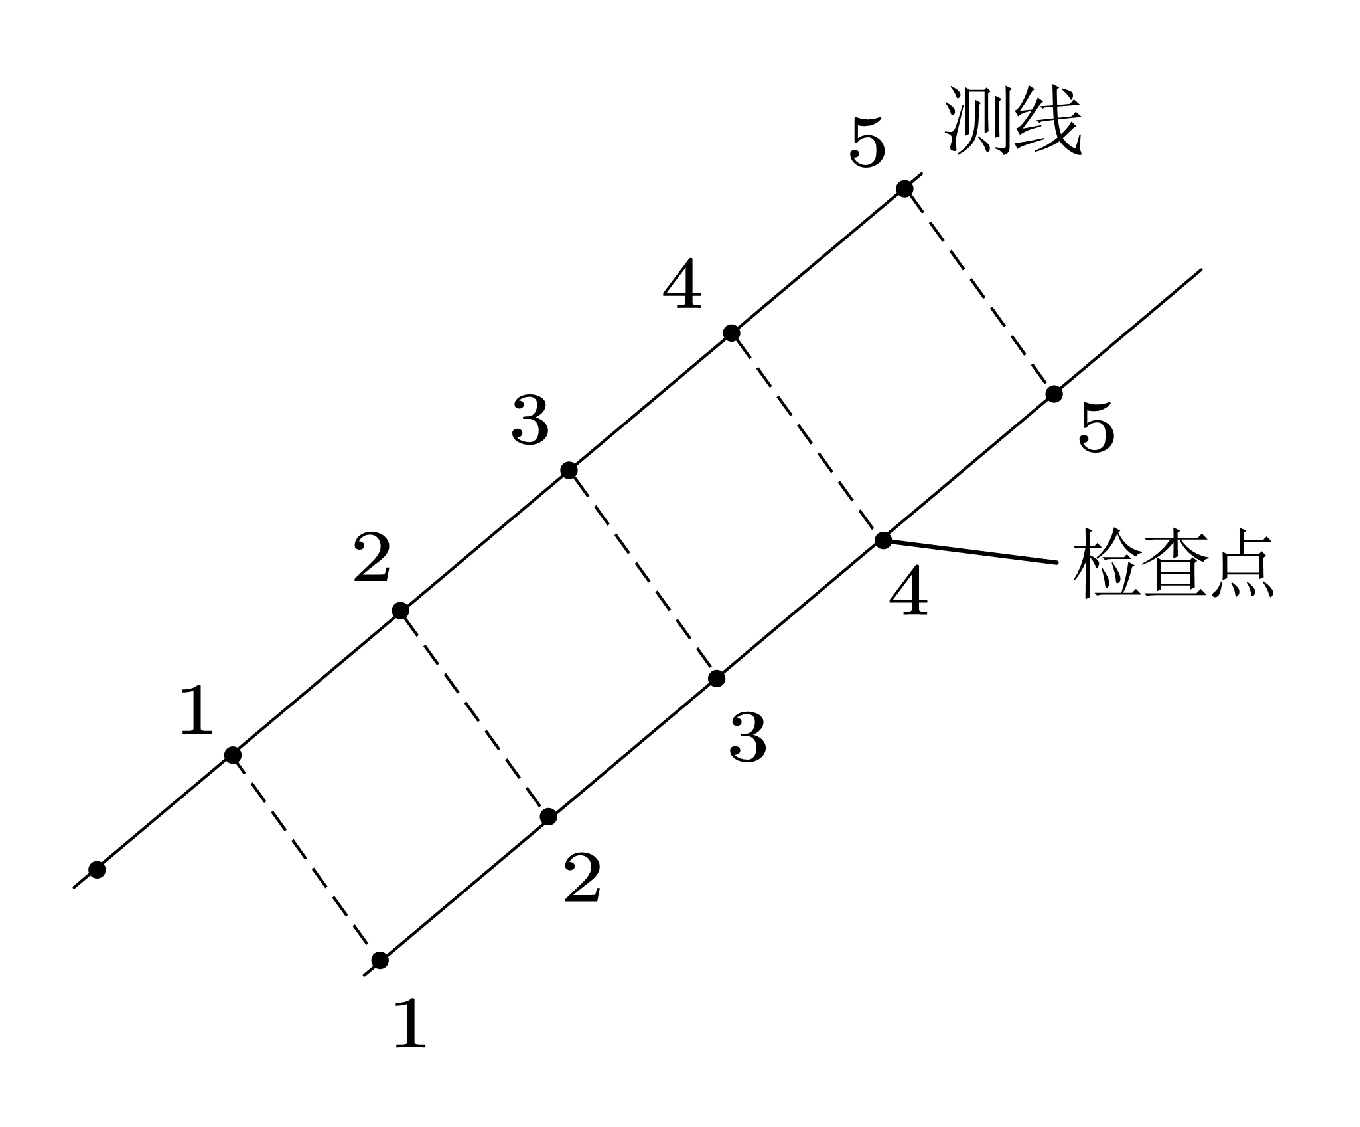
\includegraphics[width=.5\textwidth]{parallel_match}
            \caption{相邻测线检查点的匹配}
            \label{fig:parallel_match}
        \end{figure}

        
        配对完成后,我们可以给出每对检查点发出波束形成的共四个边界点(海面投影坐标),这四个边界点可近似认为在同一直线上(海面投影坐标),如\cref{fig:link_sea_bed}:
        \begin{figure}[H]
            \centering
            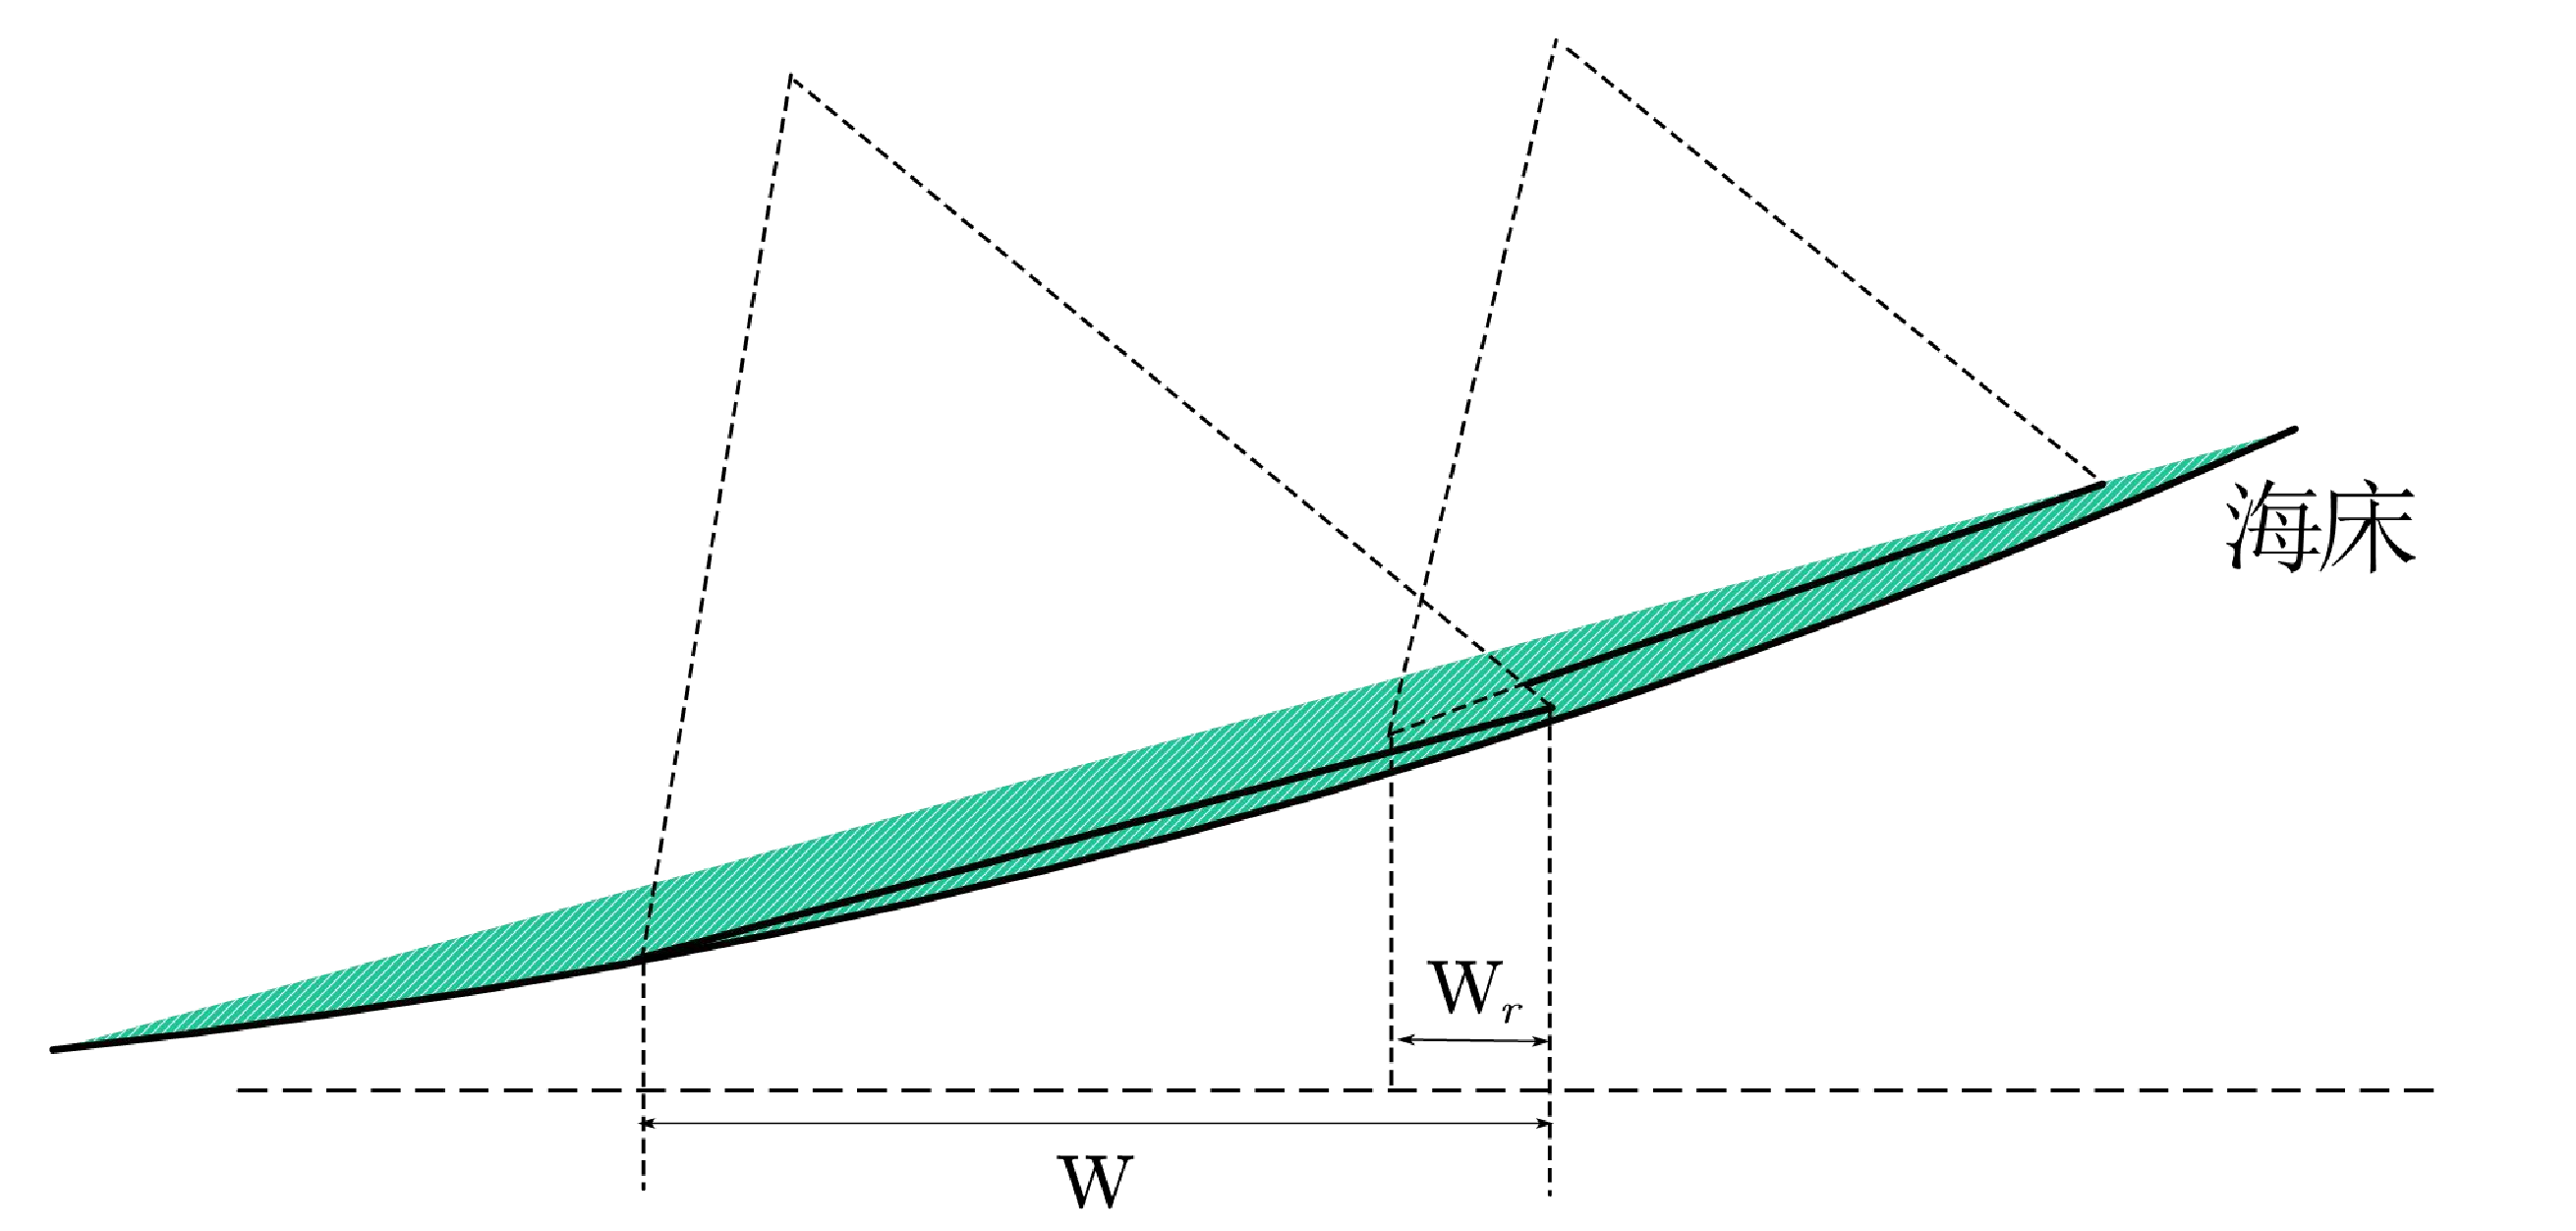
\includegraphics[width=.65\textwidth]{link_sea_bed}
            \caption{不规则海底的覆盖宽度示意}
            \label{fig:link_sea_bed}
        \end{figure}
        因此,可利用边界点坐标(海面投影坐标)计算出当前检查点对相应的重叠率 $\eta = \frac{W_r}{W}$。
        统计$\eta$大于$20\%$的检查点数量,将该数量乘以检查点间距可得当前测线重叠率高于$20\%$部分的长度。

        再考虑相邻测线间不完全平行的情况,实际问题中的测线间角度只可能为较小值,故仍沿用平行情况中使用的检查点匹配方法,并将边界点坐标再次投影到垂直
        测线方向,再使用上述方法计算每对检查点处的重叠率 $\eta$。全面积重叠率仍由式\cref{eq:eta_S}给出。
 
        \subsubsection{模型准备:漏测率计算方法}
        在布线方案相对合理的情况下,发生漏测的原因主要有两种:

        1. 由于测线不平行于海域边界,若不对边界做特殊处理,会导致边界区域出现漏测。

        2. 由于海底地形的复杂性,可能出现某条测线的某一部分的覆盖宽度突然异常减小的情况,进而发生漏测。
        
        对于第一类漏测情况,本文采取主动处理的方式,通过细化边界处理方案来解决,也可在必要时增加沿边界的补漏测线。

        本文主要讨论第二种漏测情况的漏测面积计算方法,并作如下假设:

        1. 对海底的每个点只考虑与其距离最近的两条测线上可能发出的波束,不考虑其他测线可能造成的影响,即不考虑两条测线间漏测区域被其他测线波束覆盖或与其他测线的漏测区重叠的情况。

        2. 已对边界进行处理并保证测线布设方案的相对合理,保证漏测区域仅可能在某两条测线之间。

        以上假设将在模型检验中详细讨论。

        本文沿用计算覆盖率的方法,先对两条测线做检查点配对,再计算每对检查点对应的未覆盖宽度(若无则计为0),利用$S_{\varepsilon} = \sum_{1}^{n} W_{\varepsilon_i} \Delta l$计算漏测面积,
        进而计算漏测海区占总待测海域面积的百分比(漏测率):
        \begin{equation}
            \epsilon = \frac{S_\varepsilon}{S_{a}}
            \label{epsilon}
        \end{equation}
        其中 $S_a$ 为待测海域总面积。

        \subsubsection{通用方法:基于贪心算法的布线策略}
        本问的目标是给出总测线长度、超过20\%重叠率的测线长度以及漏测率均较优的布线方案。假设已找到了一条较好的初始测线,则下一条理想测线应尽可能保证与初始测线的重叠率较小,且尽可能不发生漏测。
        考虑到沿测线方向各检查点深度不同,沿垂直测线的近似爬升率也不同,且并无确定规律,故没有确定的策略可保证每个检查点处重叠率最小或不发生漏测,只能通过以下措施尽可能保证各点的重叠率、
        漏测率均较小:

        1. 根据问题三的分析与结论,当测线方向上深度变化过于剧烈时,不可能同时满足低漏测率与低重叠率的要求。尽可能沿等深线方向设置测线可以保证测线上各检查点的深度较为相似,有利于
        低重叠率与低漏测率的实现。因此,可选取恰能覆盖边界且与等深线方向较为接近、爬升率较小的测线作为初始测线。

        2. 根据等高线图与高度分布图可知,测线两端点一般为该测线的较高点与较低点。
        根据
        $W \approx D\sin\frac{\theta}{2}(\frac{1}{\cos(\frac{\theta}{2}+\hat{\gamma})} + \frac{1}{\cos(\frac{\theta}{2} - \hat{\gamma})})\cos\hat{\gamma}$,
        其中 $\hat{\gamma}$ 为垂直测线方向爬升角的估计值。
        在测线两端点处根据某一固定重叠率确定下一条测线的两端点时,其他检查点对应的覆盖宽度$W_i$大部分在两端点对应的覆盖宽度之间,可知逐点覆盖率也大致在该固定重叠率附近。
        故可根据该固定重叠率与测线两端点处覆盖宽度来确定下一较优测线的位置。以下给出基于该策略的具体方案。

        \subsubsection{基础方案:端点处重叠率一致的布线方案}
        将海平面作为一个整体,在最深端(海域东南角附近)确定第一条测线后,根据两端点处的覆盖宽度 $W$ 与端点处重叠率 $\eta$,确定两个新的端点形成下一条测线。
        以此类推,直到覆盖海域的另一侧边界。

        该方案在确定任何区域的测线时都使用相同的端点处重叠率,该重叠率的大小对总测线长度、超过20\%重叠率测线长度、漏测率均有较大影响。
        
        本文对$3\% \sim 16\%$的端点处重叠率进行搜索,得到端点处重叠率大小与总测线长度、超过20\%重叠率的测线长度、漏测率的关系图如下:
        \begin{figure}[H]
            \centering
            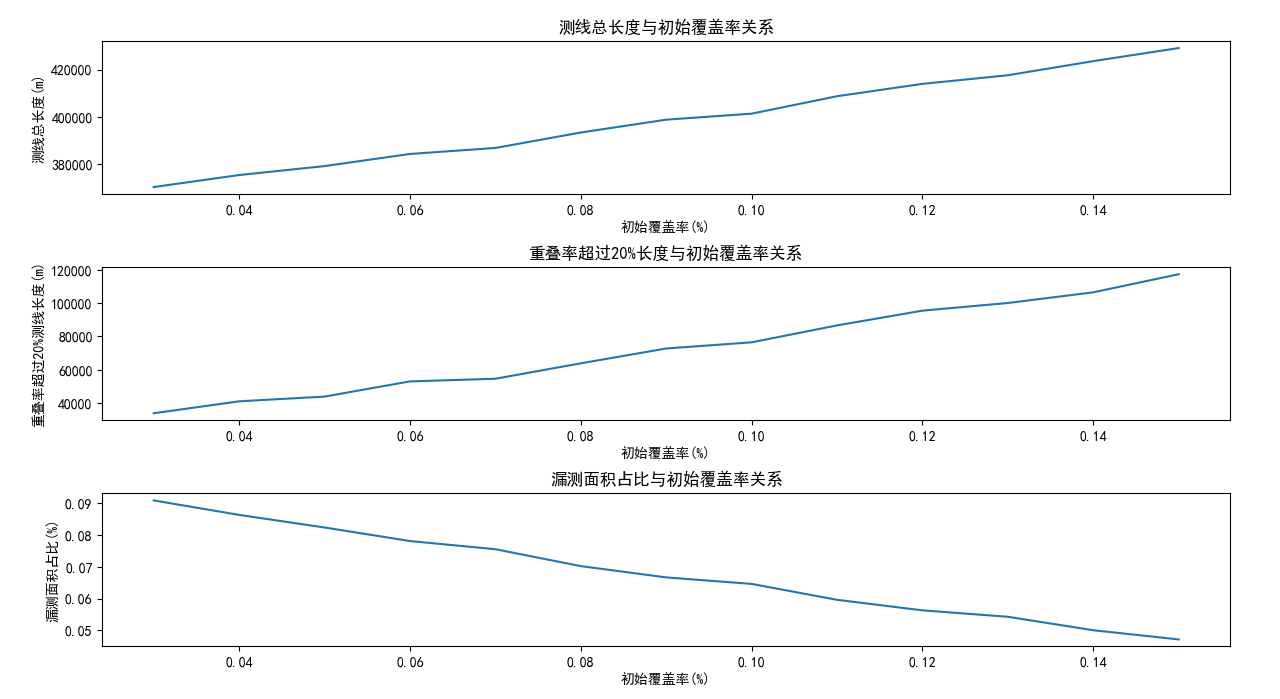
\includegraphics[width=.95\textwidth]{result_3}
            \caption{端点处重叠率对三种指标的影响}
            \label{fig:result_3}
        \end{figure}
        由\cref{fig:result_3}可知,当要求漏测率在5\%以下,端点处重叠率必须在12\%以上,此时超过20\%重叠率的测线长度比例在20\%以上,已造成了较大的数据冗余。

        以下是端点处重叠率为10\%时的条带可视化图,其中蓝色区域表示该区域已被测量,红色纹状区域表示该处重叠率大于20\%,白色区域表示该区域被漏测。
        \begin{figure}[H]
            \centering
            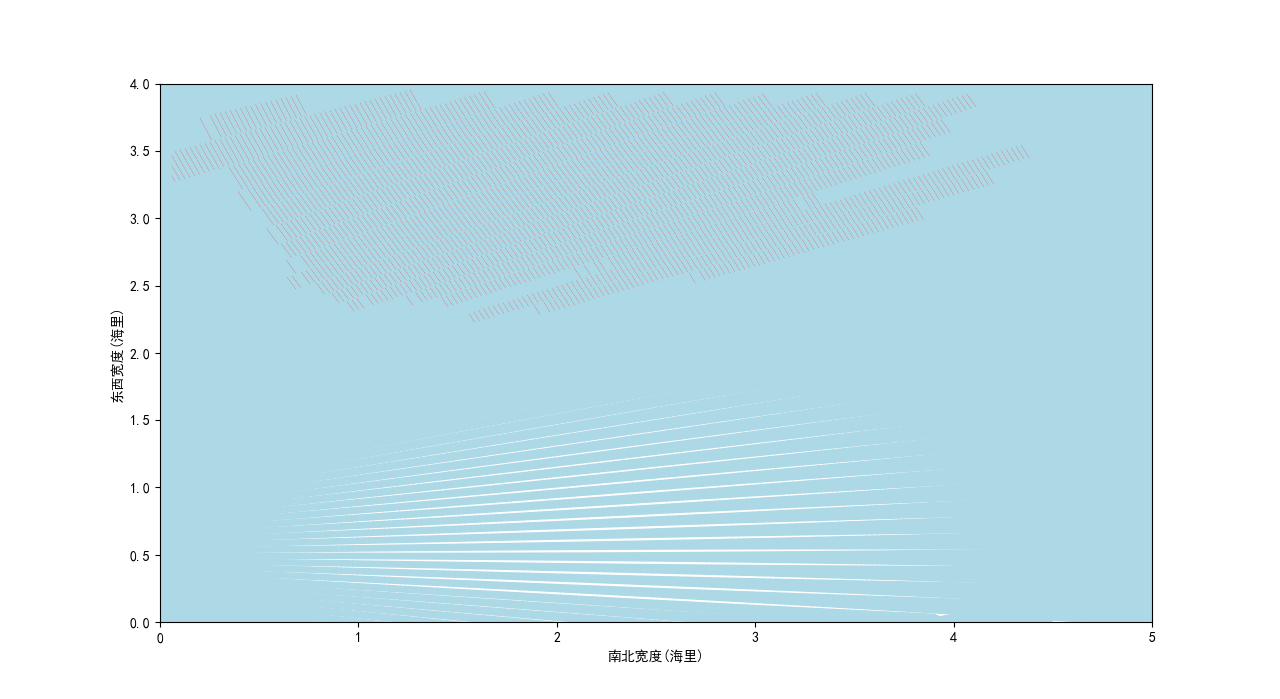
\includegraphics[width=.9\textwidth]{dyn_0}
            \caption{基础方案条带覆盖图}
            \label{fig:dyn_0}
        \end{figure}

        \subsubsection{优化方案一:基于动态端点处重叠率的布线方案}
        分析\cref{fig:result_3}可得,由于方案一中只能设置固定的端点处重叠率,无法灵活处理不同区域的特征差异,导致部分区域冗余严重、部分区域漏测严重的现象。
        考虑相邻测线间地形的局部相似性,本文考虑动态调整端点处重叠率:

        1. 当前测线与前一条测线之间有超过20\%重叠率的部分时,将端点处重叠率略微调小。

        2. 当前测线与前一条测线之间有漏测部分时,将端点处重叠率略微调大。

        3. 否则,继续使用当前的端点处重叠率。

        4. 其他策略与基础方案一致。
        
        该方案保证不会出现大面积的聚集性漏测或冗余,能更好适应地形特征。

        该方案可以优化的参数为端点处重叠率初始值 $\eta_0 $。本文将重叠率的调整幅度设为$1\%$,距离最深处海域边界线的起始点设为 $3.9$(海里)。
        通过\textbf{等距搜索法}得到最优端点处重叠率初始值为 $\eta_0 = 0.02$,
        最终测线分布图如\cref{fig:line_1}:
        \begin{figure}[H]
            \centering
            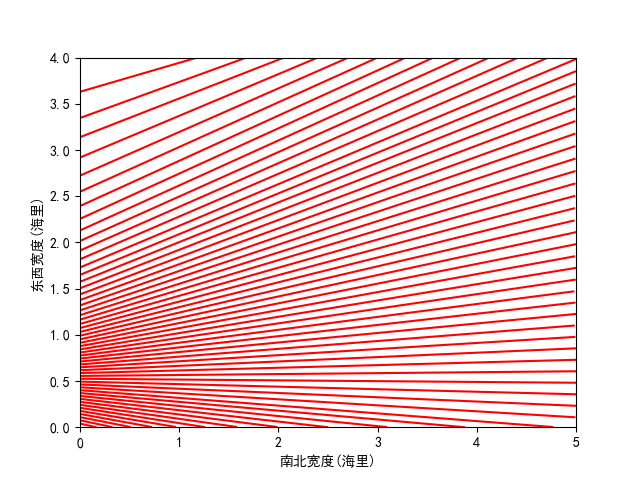
\includegraphics[width=.9\textwidth]{line_1}
            \caption{优化方案一测线分布图}
            \label{fig:line_1}
        \end{figure}
        条带覆盖图如\cref{fig:dyn_1}:
        \begin{figure}[H]
            \centering
            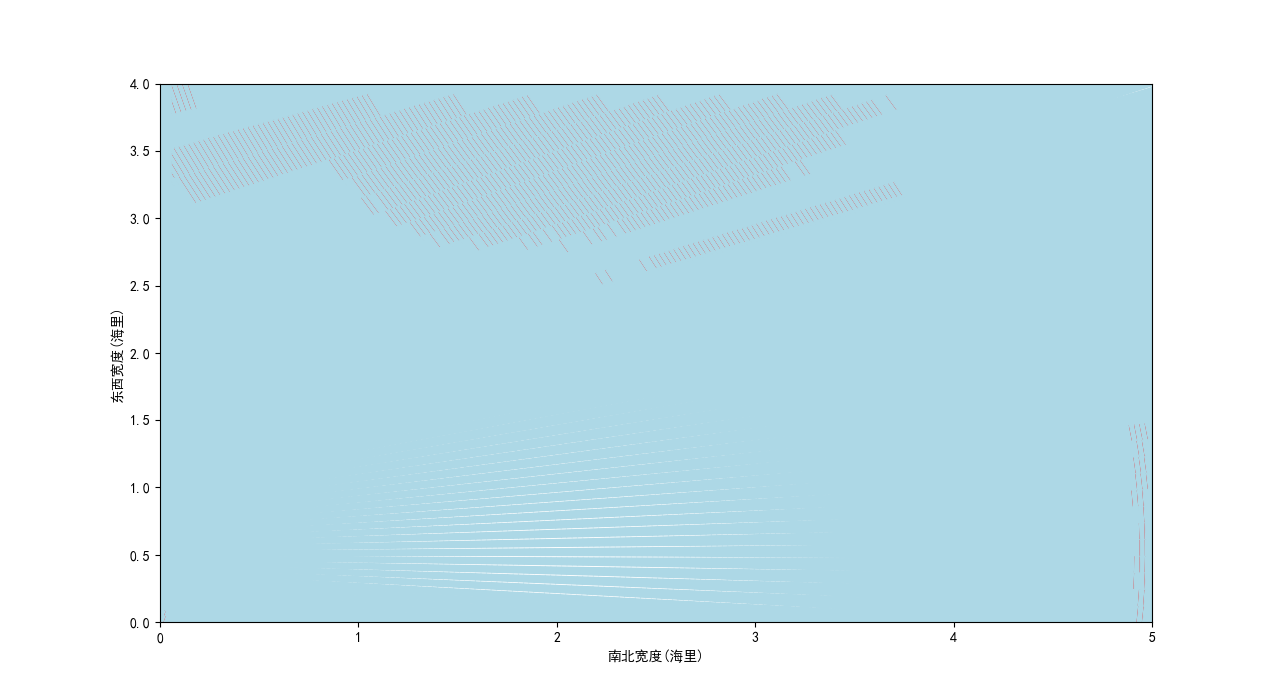
\includegraphics[width=.9\textwidth]{dyn_1}
            \caption{优化方案一条带覆盖图}
            \label{fig:dyn_1}
        \end{figure}
        其中蓝色区域表示该区域已被测量,红色纹状区域表示该处重叠率大于20\%,白色区域表示该区域被漏测。
       
        各指标结果如下:
        \textbf{测线总长度}为:$414100$m,\textbf{漏测海区占总待测海域面积的百分比}:$3.58\%$,\textbf{重叠率超过 $20\%$ 部分的总长度}:$39600$m。
        \subsubsection{优化方案二:基于海域划分的布线方案}
        基础方案的不足在于无法处理不同海域的地形特征差异,故另一种思路是将海域划分为不同的区域处理:

        1. 先使用基础方案逐步确定最优测线,直到连续5条测线没有出现超过20\%重叠率的区域,此时认为海域性质发生变化,沿该测线将已确定测线区域与未确定测线区域
        划分为两个海域。

        2. 为多个海域中分别选取合适的端点处重叠率,将海域分界线作为新海域的起始测线,按当前海域的端点处重叠率继续确定其他测线,直到所有海域的测线都确认完毕。

        3. 其他策略与基础方案一致。

        该方案有较强的抗干扰性,能从整体上适应地形特征。

        该方案可以优化的参数为不同海域的端点处重叠率,本文将海域划分成两个海域,考虑到只有两个参数可以优化,本文运用等距搜索法,
        搜得两片海域最优初始端点处重叠率分别为$\eta_1 = 0.02$与$\eta_2 = 0.15$。
        海域划分图如\cref{fig:sea_bed_part}:
        \begin{figure}[H]
            \centering
            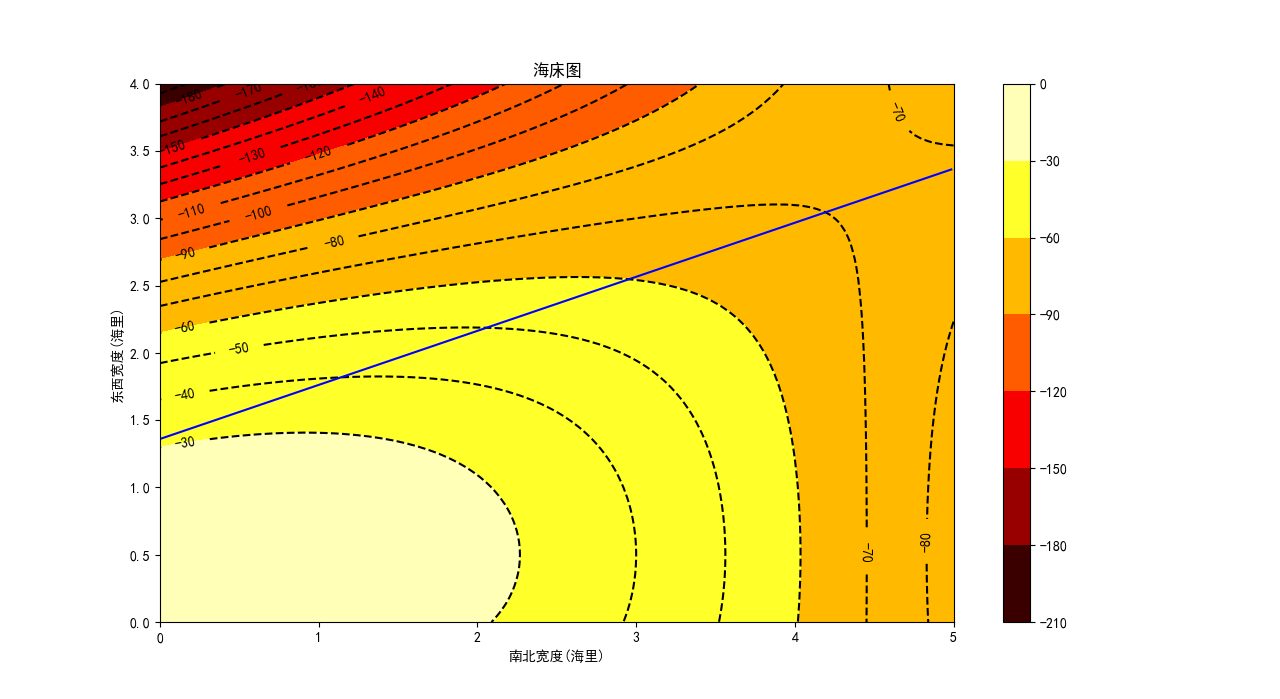
\includegraphics[width=.9\textwidth]{sea_bed_part}
            \caption{海域划分图}
            \label{fig:sea_bed_part}
        \end{figure}
        测线分布图如\cref{fig:line_2}:
        \begin{figure}[H]
            \centering
            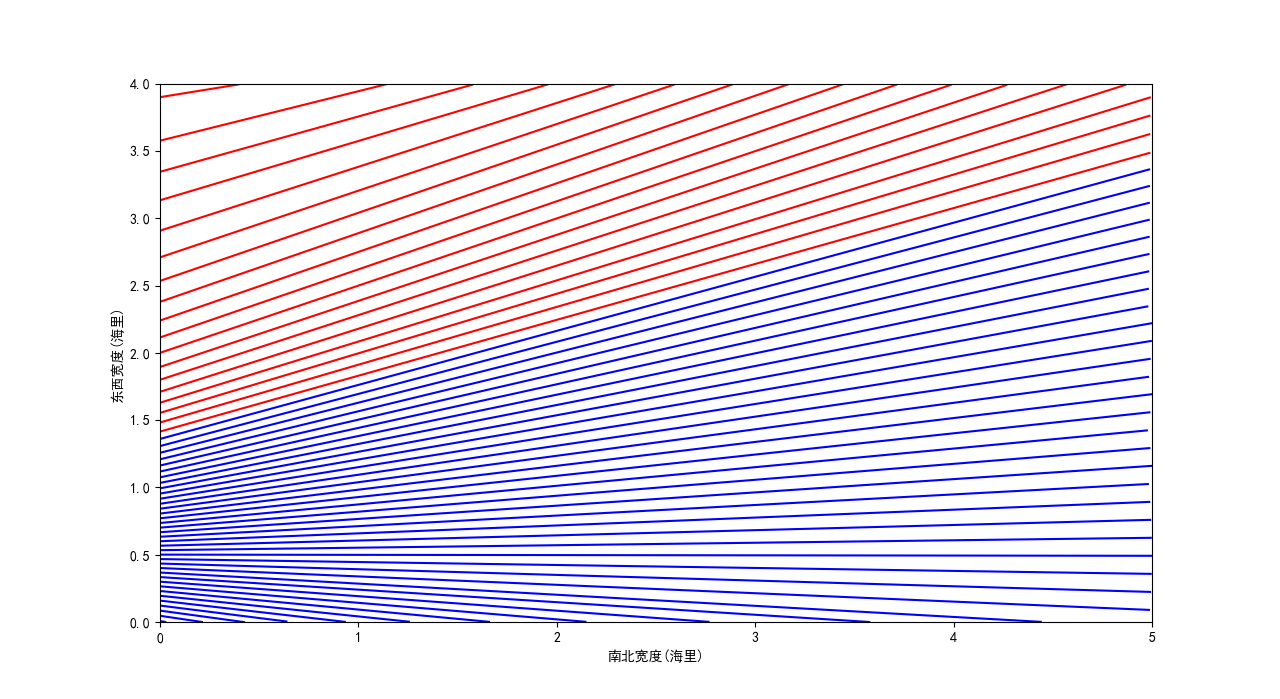
\includegraphics[width=.9\textwidth]{line_2}
            \caption{优化方案二测线分布图}
            \label{fig:line_2}
        \end{figure}
        条带覆盖图如\cref{fig:dyn_2}:
        \begin{figure}[H]
            \centering
            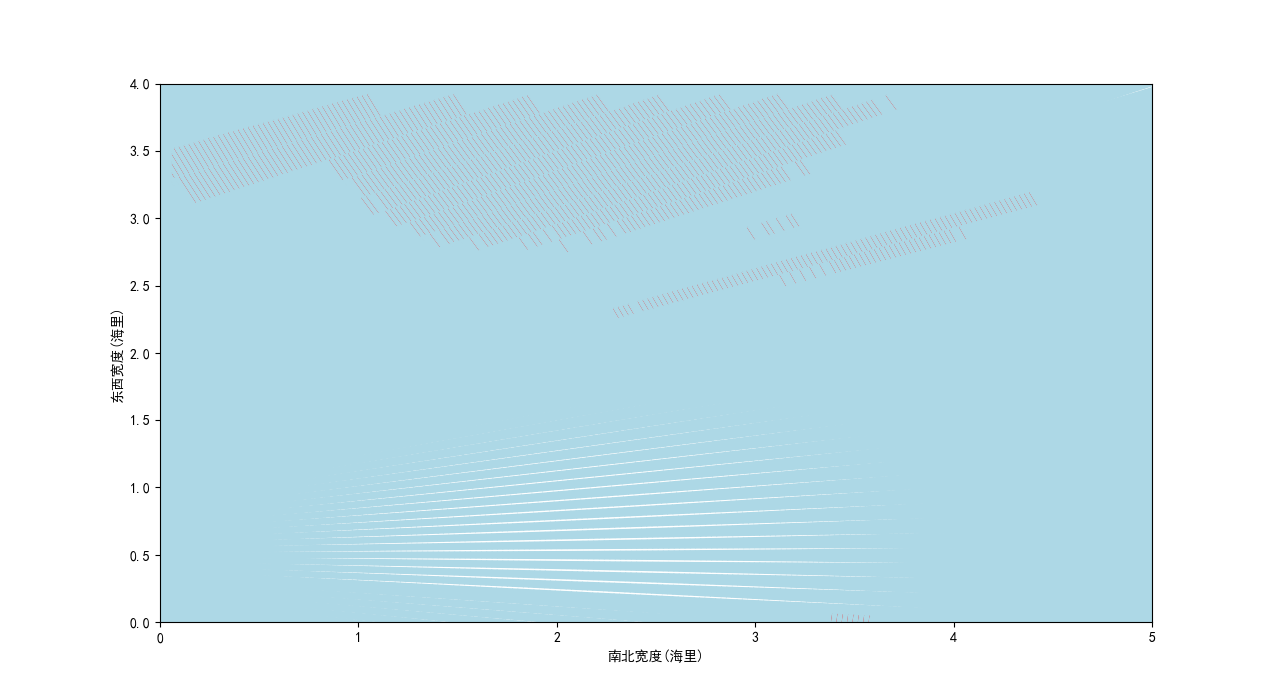
\includegraphics[width=.9\textwidth]{dyn_2}
            \caption{优化方案二条带覆盖图}
            \label{fig:dyn_2}
        \end{figure}
        各指标结果如下:
        \textbf{测线总长度}为:$407050$m,\textbf{漏测海区占总待测海域面积的百分比}:$4.73\%$,\textbf{重叠率超过 $20\%$ 部分的总长度}:$40600$m。

        \subsubsection{求解结果}
        综上所述,优化方案二在满足约束条件下测线总长度达到最小。
        结果如下:
        \textbf{测线总长度}为:$407050$m,\textbf{漏测海区占总待测海域面积的百分比}:$4.73\%$,\textbf{重叠率超过 $20\%$ 部分的总长度}:$40600$m。

        \section{模型的分析与检验}
        \subsection{问题四中误差来源的分析}
        问题四中建立的模型使用了较多近似方法,给出完整误差分析较为困难,故只对误差来源进行分析:

        1. 海底深度数据是离散的,故条带面积数据与真实条带面积存在误差。

        2. 计算覆盖宽度时,为降低计算量未使用投影方法,而使用了近似方法,该方法对异常深度值较为敏感,误差可控性不高。
        
        3. 计算相邻测线的条带重叠率时,离散化为计算匹配点对的覆盖宽度重叠率加权值,在相邻测线角度较大时可能因系统性误差而导致重叠率偏高。

        \subsection{问题四中部分近似方法的合理性检验}
            1.问题四中对每条测线每50米设置一个检查点,用于估计当前测线形成的条带面积。问题四中深度数据的分辨率为0.02海里,即31.64米,这与测线上检查点的间距匹配,基本可
            保证每个检查点计算覆盖宽度时候可以选到不同点,且被跳过的深度数据较少,可知该检查点间距合理。
            
            2.问题四中动态调整端点处重叠率的方案中,假设相邻测线间未被覆盖的区域不会被其他测线覆盖。通过数据分析,所有测线间的逐点重叠率均在100\%以下,即任意测线的外侧波束不可能
            越过相邻波束的另一侧,可知原假设合理。
        
        


        \section{模型的评价、改进与推广}
        \subsection{模型的优点}
        \begin{enumerate}
            \item 理想海底面的测线最优布设方案模型由严谨的几何分析得出,具有较高的可靠性、通用性与可解释性。
            \item 使用贪心算法,将复杂的全局优化问题转化为多步局部优化问题,极大降低了问题的复杂性,使模型简洁高效。
            \item 非理想海底面的测线最优布设方案充分考虑了海底地形特征的区域性,结合理论与数值模拟方法,使模型有较好的适用性。
        \end{enumerate}

        \subsection{模型的缺点}
        \begin{enumerate}
            \item 非理想海底面情形下各指标的数值计算方法误差来源较复杂,不便进行误差分析。
            \item 对海域边界的处理较为粗糙,不利于模型的推广。
            \item 对海域划分的方式较为简单,未给出更通用的海域划分方式。
        \end{enumerate}
        

        \subsection{模型的改进}
        \begin{enumerate}
            \item 将初始测线的选取作为优化问题求解,尽可能给出较好的初始测线。
            \item 使用聚类方法,以海深、等深线方向与密度作为聚类特征,给出更具可解释性的海域划分方式。
            \item 细化端点处重叠率更新的方式,如引入动量法等。
            \item 可先适当降低覆盖率的要求,通过加入补测线的方式覆盖主测线未覆盖的部分,再比较新方案与原方案的测线长度。
        \end{enumerate}
        
    

        \subsection{模型的推广}
        本文基于几何分析方法与贪心算法,给出了一种多波束测深测线最优布线方案。该工作可以被推广到其他场景下的测线布设,如海洋磁力测量、卫星测量等。
        本文也可应用于相似的路径规划问题,如无人机灌溉等场景。
        \begin{thebibliography}{9}%宽度9
            \bibitem[1]{bib_1}
            陈立家,王凯,吴小红等.
            \newblock 船舶运动模型的处理方法、装置及存储介质\allowbreak[P].
            \newblock 湖北省:CN114384821A,2022-04-22.
            \bibitem[2]{bib_2}
            王闰成,黄永军.
            \newblock 多波束测深外业实施研究\allowbreak[J].
            \newblock 海洋测绘,2007(03):66-70.
            \bibitem[3]{bib_3}
            张明亮,许家琨,苏振礼等.
            \newblock 多波束水深测量规范框架研究\allowbreak[J].
            \newblock 海洋测绘,2009,29(03):47-49.
            \bibitem[4]{bib_4}
            邹永刚,贾俊涛,翟京生等.
            \newblock 多波束系统波束宽度对水深点不确定度影响分析\allowbreak[J].
            \newblock 辽宁工程技术大学学报(自然科学版),2011,30(01):68-72.
        \end{thebibliography}
        \newpage
        \begin{appendices}
            \section{支撑材料}
            \begin{lstlisting}
            other.py
            question1.py
            question2.py
            question3.py
            question3_1.py
            question4.py
            save_result.py
            result1.xlsx
            result2.xlsx
            图片文件夹figure
            \end{lstlisting}
            \section{问题一}

            \begin{lstlisting}[language=python]
            import numpy as np
            from save_result import pd_toexcel1
            
            theta = np.pi / 3  # 半开角
            alpha = 1.5 / 180 * np.pi  # 坡度
            d = 200  # 测线间隔
            
            def cal(x, d):
                """计算深度、覆盖宽度、覆盖率"""
                D = 70 - d * x * np.tan(alpha)# 深度 
                W = D * np.sin(theta) * (1 / np.cos(theta - alpha) + 1 / np.cos(theta + alpha)) * np.cos(alpha) # 覆盖宽度
                eta = 1 - (d / W) * (np.cos(theta) * np.cos(alpha) / np.cos(theta - alpha))  # 覆盖率
                return D, W, eta
            
            Data = np.zeros((9, 3))
            for x in range(-4, 5):
                D, W, eta = cal(x, d)
                res = np.array([D, W, eta])
                Data[x + 4] = res
            
            # 保存结果
            pd_toexcel1(Data, 'result1.xlsx')
            \end{lstlisting}

            \section{问题二}

            \begin{lstlisting}[language=python]
            import numpy as np
            from save_result import pd_toexcel2
            
            theta = np.pi / 3  # 半开角
            alpha = 1.5 / 180 * np.pi  # 坡度
            D = 120  # 海域中心深度
            d = 0.3 * 1852# 步长
            
            def cal_w(x, beta):
                """计算深度、覆盖宽度"""
                gamma = np.arctan(np.sin(beta) * np.tan(alpha))  # 测线斜波交线和投影夹角
                tan_phi = -np.cos(beta) * np.tan(alpha)  # 爬升角
                D = 120 - d * x * tan_phi# 深度 
                W = D * np.sin(theta) * (1 / np.cos(theta - gamma) + 1 / np.cos(theta + gamma)) * np.cos(gamma) # 覆盖宽度
                return D, W
            
            Data = np.zeros((8, 8))
            for x in range(8):
                j = 0
                for b in np.arange(0 , 360 , 45) * np.pi / 180:
                    _, W = cal_w(x, b)
                    Data[x, j] = W
                    j += 1
            
            # 保存结果
            pd_toexcel2(Data, 'result2.xlsx')
            \end{lstlisting}

            \section{问题三 —— 逐点覆盖率}
            \begin{lstlisting}[language=python]
            import numpy as np
            import matplotlib.pylab as plt

            theta = np.pi / 3  # 半开角
            alpha = 1.5 / 180 * np.pi  # 坡度
            d = 200  # 测线间隔
            eta = 0.1 # 最小覆盖率

            def depth(x):
                """计算深度"""
                return - 110 - (x - 2 * 1852) * np.tan(alpha)


            def dx(x, y, beta):
                """更新下一个测线最高点的坐标"""
                gamma = np.arcsin(np.sin(beta) * np.tan(alpha))  # 测线斜波交线和投影夹角
                z = depth(y)  # 深度
                W = np.abs(z) * np.sin(theta) * (1 / np.cos(theta - gamma) + 1 / np.cos(theta + gamma)) * np.cos(gamma) # 覆盖宽度
                N = np.abs(z) * np.sin(theta) * 1 / np.cos(theta + gamma) * np.cos(gamma) # 平分线一侧覆盖宽度
                y_1 = y + N * np.cos(beta - np.pi / 2) - W * eta
                L = N - W * eta + np.abs(depth(y_1)) * np.tan(np.pi / 3)
                if x < 2 * 1852:
                    x_new = x + L / np.sin(beta - np.pi / 2) 
                    y_new = y
                    if x_new > 2 * 1852:
                        y_new = (x_new - 2 * 1852) * np.tan(beta - np.pi / 2)
                        x_new = 2 * 1852
                else :
                    x_new = x
                    y_new = y + L / np.cos(beta - np.pi / 2)
                return x_new, y_new


            def init(beta):
                """初始化第一条测线坐标"""
                gamma = np.arctan(np.sin(beta) * np.tan(alpha))  # 测线斜波交线和投影夹角
                z = depth(0)  # 深度
                M = np.abs(z) * np.sin(theta) * 1 / np.cos(theta - gamma) * np.cos(gamma) # 平分线一侧覆盖宽度
                if beta == np.pi / 2:
                    x = np.inf
                else:
                    x = M / np.sin(beta - np.pi / 2)
                if x < 2 * 1852:
                    return x, 0
                else:
                    y = np.abs(z) * np.tan(np.pi / 3)
                    return 2 * 1852, y
                
            def far_y(y, beta):
                """测线侧量的最远点坐标"""
                gamma = np.arctan(np.sin(beta) * np.tan(alpha))  # 测线斜波交线和投影夹角
                z = depth(y)  # 深度
                N = np.abs(z) * np.sin(theta) * 1 / np.cos(theta + gamma) * np.cos(gamma) # 平分线一侧覆盖宽度
                return y + N * np.cos(beta - np.pi / 2)

            def map(x, y, beta):
                """计算当前测线最低点坐标"""
                if x < 2 * 1852:
                    return 0, np.tan(beta - np.pi / 2) * x
                else :
                    return 0, y + 2 * 1852 * np.tan(beta - np.pi / 2)


            def sum_len(beta):
                """计算测线总长度"""
                x, y = init(beta)
                sum = 0
                while x <= 2 * 1852 and far_y(y,beta) <= 4 * 1852:
                    x_1, y_1 = map(x, y, beta)
                    sum += np.sqrt((x_1 - x) ** 2 + (y_1 - y) ** 2)
                    x, y = dx(x, y, beta)
                x_1, y_1 = map(x, y, beta)
                sum += np.sqrt((x_1 - x) ** 2 + (y_1 - y) ** 2)
                return sum


            def is_true(beta):
                """判断是否是合格的测线"""
                gamma = np.arcsin(np.sin(beta) * np.tan(alpha))  # 测线斜波交线和投影夹角
                x, y = init(beta)
                _, y_0 = map(x, y, beta)
                y_f = y_0
                flag = True
                while x <= 2 * 1852 and y <= 4 * 1852:
                    _, y_1 = map(x, y, beta)
                    if y_f != y_0:
                        d = (y_1 - y_f) * np.cos(beta - np.pi / 2)
                        z_f = depth(y_f)
                        W = np.abs(z_f) * np.sin(theta) * (1 / np.cos(theta - gamma) + 1 / np.cos(theta + gamma)) * np.cos(gamma) # 覆盖宽度
                        eta = 1 - (d / W) * (np.cos(theta) * np.cos(gamma) / np.cos(theta - gamma))  # 覆盖率
                        if eta > 0.2:
                            flag = False
                    y_f = y_1
                    x, y = dx(x, y, beta)
                return flag


            def show_line(beta):
                """绘制当前测线"""
                X = np.array([])
                Y = np.array([])
                x, y = init(beta)
                plt.plot((0, 4 * 1852),(0, 0), color = 'gray')
                plt.plot((4 * 1852, 4 * 1852),(0, 2 * 1852), color = 'gray')
                plt.plot((4 * 1852, 0),(2 * 1852, 2 * 1852), color = 'gray')
                plt.plot((0, 0),(2 * 1852, 0), color = 'gray')
                while x <= 2 * 1852 and far_y(y,beta) <= 4 * 1852:
                    x_1, y_1 = map(x, y, beta)
                    plt.plot((y,y_1),(x,x_1), color = 'red')
                    # plt.plot((far_y(y,beta),far_y(y_1,beta)),(x,x_1), color = 'blue')
                    X = np.append(X, x)
                    Y = np.append(Y, y)
                    x, y = dx(x, y, beta)
                x_1, y_1 = map(x, y, beta)
                plt.plot((y,y_1),(x,x_1), color = 'red')
                # plt.plot((far_y(y,beta),far_y(y_1,beta)),(x,x_1), color = 'blue')


            if __name__ == '__main__':
                BETA = np.arange(90, 180, 0.01)
                # 求符合覆盖率的角度范围
                for beta in BETA:
                    if(is_true(beta * np.pi / 180)):
                        continue
                    else:
                        high_beta = beta
                        break
                ans = np.array([])
                low = np.inf
                low_beta = 0
                print('最大可行角度为:' + str(high_beta) + '°')
                BETA = np.arange(90, high_beta - 0.01, 0.001)
                # 求最短测线路径
                for beta in BETA * np.pi / 180:
                    ans_now = sum_len(beta)
                    ans = np.append(ans, ans_now)
                    if ans_now < low:
                        low = ans_now
                        low_beta = beta
                print('最佳测线方向夹角为:' + str(low_beta * 180 / np.pi) + '°')
                print('最短测线总长度为:' + str(low) + 'm')
                plt.rc('font',family='SimHei')
                plt.plot(BETA, ans)
                plt.xlabel('测线方向夹角(°)')
                plt.ylabel('测线总长度(m)')
                plt.title('测线总长度与测线方向夹角关系')
                plt.figure()
                # 绘制测线路径
                show_line(low_beta)
                plt.xlabel('东西宽度(m)')
                plt.ylabel('南北宽度(m)')
                plt.title('测线路径')
                plt.show()

            \end{lstlisting}

            \section{问题三 —— 全面积覆盖率}
            \begin{lstlisting}[language=python]
            import numpy as np
            import matplotlib.pylab as plt
            
            theta = np.pi / 3  # 半开角
            alpha = 1.5 / 180 * np.pi  # 坡度
            d = 200  # 测线间隔
            eta = 0.1
            
            def depth(x):
                """计算深度"""
                return - 110 - (x - 2 * 1852) * np.tan(alpha)
            
            
            def map(x, y, beta):
                """计算当前测线最低点坐标"""
                if x < 2 * 1852:
                    return 0, np.tan(beta - np.pi / 2) * x
                else :
                    return 0, y + 2 * 1852 * np.tan(beta - np.pi / 2)
            
            
            def dx(x, y, beta):
                """更新下一个测线最高点的坐标"""
                gamma = np.arcsin(np.sin(beta) * np.tan(alpha))  # 测线斜波交线和投影夹角
                x_1, y_1 = map(x, y, beta)
                z = depth(y)  # 深度
                z_1 = depth(y_1)
                W = np.abs(z) * np.sin(theta) * (1 / np.cos(theta - gamma) + 1 / np.cos(theta + gamma)) * np.cos(gamma) # 覆盖宽度
                M = np.abs(z) * np.sin(theta) * 1 / np.cos(theta - gamma) * np.cos(gamma) # 平分线一侧覆盖宽度
                W_1 = np.abs(z_1) * np.sin(theta) * (1 / np.cos(theta - gamma) + 1 / np.cos(theta + gamma)) * np.cos(gamma) # 覆盖宽度
                d = (W + W_1) * 9 / 20
                y_2 = y + (d - M) * np.cos(beta - np.pi / 2)
                L = d - M + np.abs(depth(y_2)) * np.tan(np.pi / 3)
                if x < 2 * 1852:
                    x_new = x + L / np.sin(beta - np.pi / 2) 
                    y_new = y
                    if x_new > 2 * 1852:
                        y_new = (x_new - 2 * 1852) * np.tan(beta - np.pi / 2)
                        x_new = 2 * 1852
                else :
                    x_new = x
                    y_new = y + L / np.cos(beta - np.pi / 2)
                return x_new, y_new, (d - M) / np.tan(beta - np.pi / 2) 
            
            
            def init(beta):
                """初始化第一条测线坐标"""
                gamma = np.arctan(np.sin(beta) * np.tan(alpha))  # 测线斜波交线和投影夹角
                z = depth(0)  # 深度
                M = np.abs(z) * np.sin(theta) * 1 / np.cos(theta - gamma) * np.cos(gamma) # 平分线一侧覆盖宽度
                x = M / np.sin(beta - np.pi / 2)
                if x < 2 * 1852:
                    return x, 0
                else:
                    y = np.abs(z) * np.tan(np.pi / 3)
                    return 2 * 1852, y
                
            def far_y(y, beta):
                gamma = np.arctan(np.sin(beta) * np.tan(alpha))  # 测线斜波交线和投影夹角
                z = depth(y)  # 深度
                N = np.abs(z) * np.sin(theta) * 1 / np.cos(theta + gamma) * np.cos(gamma) # 平分线一侧覆盖宽度
                return y + N * np.cos(beta - np.pi / 2)
            
            def low_y(y, beta):
                gamma = np.arctan(np.sin(beta) * np.tan(alpha))  # 测线斜波交线和投影夹角
                z = depth(y)  # 深度
                M = np.abs(z) * np.sin(theta) * 1 / np.cos(theta - gamma) * np.cos(gamma) # 平分线一侧覆盖宽度
                return y - M * np.cos(beta - np.pi / 2)
            
            
            def sum_len(beta):
                """计算测线总长度"""
                x, y = init(beta)
                sum = 0
                _,_,d = dx(x, y, beta)
                while x <= 2 * 1852 and far_y(y,beta) <= 4 * 1852:
                    if x < 2 * 1852:
                        sum += d
                    x_1, y_1 = map(x, y, beta)
                    sum += np.sqrt((x_1 - x) ** 2 + (y_1 - y) ** 2)
                    x, y, d = dx(x, y, beta)
                x_1, y_1 = map(x, y, beta)
                sum += np.sqrt((x_1 - x) ** 2 + (y_1 - y) ** 2)
                return sum
            
            
            def is_true(beta):
                """判断是否是合格的测线"""
                gamma = np.arcsin(np.sin(beta) * np.tan(alpha))  # 测线斜波交线和投影夹角
                x, y = init(beta)
                _, y_0 = map(x, y, beta)
                y_f = y_0
                flag = True
                while x <= 2 * 1852 and y <= 4 * 1852:
                    _, y_1 = map(x, y, beta)
                    if y_f != y_0:
                        d = (y_1 - y_f) * np.cos(beta - np.pi / 2)
                        z_f = depth(y_f)
                        W = np.abs(z_f) * np.sin(theta) * (1 / np.cos(theta - gamma) + 1 / np.cos(theta + gamma)) * np.cos(gamma) # 覆盖宽度
                        eta = 1 - (d / W) * (np.cos(theta) * np.cos(gamma) / np.cos(theta - gamma))  # 覆盖率
                        if eta > 0.2:
                            flag = False
                    y_f = y_1
                    x, y, _ = dx(x, y, beta)
                return flag
            
            
            def show_line(beta):
                """绘制当前测线"""
                X = np.array([])
                Y = np.array([])
                x, y = init(beta)
                plt.plot((0, 4 * 1852),(0, 0), color = 'gray')
                plt.plot((4 * 1852, 4 * 1852),(0, 2 * 1852), color = 'gray')
                plt.plot((4 * 1852, 0),(2 * 1852, 2 * 1852), color = 'gray')
                plt.plot((0, 0),(2 * 1852, 0), color = 'gray')
                while x <= 2 * 1852 and far_y(y,beta) <= 4 * 1852:
                    x_1, y_1 = map(x, y, beta)
                    plt.plot((y,y_1),(x,x_1), color = 'red')
                    # plt.plot((far_y(y,beta),far_y(y_1,beta)),(x,x_1), color = 'blue')
                    # plt.plot((low_y(y,beta),low_y(y_1,beta)),(x,x_1), color = 'green')
                    X = np.append(X, x)
                    Y = np.append(Y, y)
                    x, y, _ = dx(x, y, beta)
                x_1, y_1 = map(x, y, beta)
                plt.plot((y,y_1),(x,x_1), color = 'red')
                # plt.plot((far_y(y,beta),far_y(y_1,beta)),(x,x_1), color = 'blue')
                # plt.plot((low_y(y,beta),low_y(y_1,beta)),(x,x_1), color = 'green')
            
            
            if __name__ == '__main__':
                BETA = np.arange(90, 180, 0.01)
                for beta in BETA:
                    if(is_true(beta * np.pi / 180)):
                        continue
                    else:
                        high_beta = beta
                        break
                ans = np.array([])
                low = np.inf
                low_beta = 0
                BETA = np.arange(90, 91.8, 0.01)
                for beta in BETA * np.pi / 180:
                    ans_now = sum_len(beta)
                    ans = np.append(ans, ans_now)
                    if ans_now < low:
                        low = ans_now
                        low_beta = beta
                print(low_beta * 180 / np.pi)
                plt.plot(BETA, ans)
                plt.figure()
                plt.grid(True)
                show_line(low_beta)
                plt.show()
                
            \end{lstlisting}

            \section{问题三最优布线情况}
            \begin{lstlisting}[language=python]
                import numpy as np
                import matplotlib.pylab as plt
                from question3 import depth
                
                
                theta = np.pi / 3  # 半开角
                alpha = 1.5 / 180 * np.pi  # 坡度
                d = 200  # 测线间隔
                eta = 0.1 # 最小覆盖率
                
                plt.rc('font',family='SimHei')
                plt.rc('axes', unicode_minus=False)
                
                x = np.arange(-2, 2, 0.02) * 1852
                y = - 110 + -x * np.tan(alpha)
                
                plt.plot(x + 2 * 1852, y)
                plt.xlabel('东西宽度(m)')
                plt.ylabel('深度(m)')
                plt.grid(True)
                
                
                # beta = np.pi / 2 的情况
                ans = np.array([])
                max_x = 4 * 1852
                x = 0
                x2 = 0
                while(x2 < max_x):
                    y = depth(x)
                    x1 = x
                    x = x + np.abs(y) * np.tan(np.pi / 3)
                    ans = np.append(ans, x)
                    y = depth(x)
                    W = np.abs(y) * np.sin(theta) * (1 / np.cos(theta - alpha) + 1 / np.cos(theta + alpha)) * np.cos(alpha) # 覆盖宽度
                    x2 = x1 + W
                    x = x2 - eta * W
                
                d = ans[1:] - ans[:-1]
                print(d)
                plt.figure()
                plt.plot(depth(ans[:-1]), d)
                plt.xlabel('深度(m)')
                plt.ylabel('两条测线间隔(m)')
                plt.title('深度和两条测线间隔的关系')
                plt.show()
                
            \end{lstlisting}


            \section{问题四}
            \begin{lstlisting}[language=python]
            import pandas as pd
            import numpy as np
            import matplotlib.pylab as plt
            from matplotlib import cm
            
            H = pd.read_excel(io='attach.xlsx',usecols='C:GU',header=1,names=None).values
            num_pr = 0
            mis_mea = 0
            over_l = 0
            l = 0
            
            def seabed_figure():
                """绘制海床图"""
                x = np.arange(0, 4 + 0.02, 0.02)
                y = np.arange(0, 5 + 0.02, 0.02)
                X , Y = np.meshgrid(x, y)
            
                plt.rc('font',family='SimHei')
                plt.rc('axes', unicode_minus=False)
                # 3D等高图
                # plt.figure()
                # ax = plt.axes(projection='3d')
                # ax.plot_surface(X, Y, -H, cmap = 'hot', edgecolor='none')
                # ax.set_xlabel('东西宽度(海里)')
                # ax.set_ylabel('南北宽度(海里)')
                # ax.set_zlabel('深度(m)')
                # plt.title('海床图')
                # 平面等高图
                plt.figure()
                cset = plt.contourf(Y,X,-H,6,cmap='hot') 
                contour = plt.contour(Y,X,-H,20,colors='k')
                plt.clabel(contour,fontsize=10,colors='k')
                plt.colorbar(cset)
                plt.xlabel('南北宽度(海里)')
                plt.ylabel('东西宽度(海里)')
                plt.title('海床图')
            
            
            def cal_gamma(x, y, z, b):
                """计算覆盖宽度线段与水平面夹角"""
                t = 1.5
                x1 = int((x - 0.75 * z * np.cos(b)) / (1852 * 0.02))
                x2 = int((x + 0.75 * z * np.cos(b)) / (1852 * 0.02))
                y1 = int((y - 0.75 * z * np.sin(b)) / (1852 * 0.02))
                y2 = int((y + 0.75 * z * np.sin(b)) / (1852 * 0.02))
                try : 
                    z1 = H[x1,y1]
                except:
                    z1 = z
                    t /= 2
                try:
                    z2 = H[x2,y2]
                except:
                    z2 = z
                    t /= 2
                gamma = np.arctan((z1 - z2) / 
                                (t * z))
                return gamma
            
            def cal_des(x, y, beta):
                '''计算终点坐标'''
                if x == 0:
                    if 4 * 1852 - y <= np.tan(beta - np.pi / 2) * 5 * 1852:
                        return (4 * 1852 - y) / np.tan(beta - np.pi / 2) ,4 * 1852
                    else:
                        return 5 * 1852, y + 5 * 1852 * np.tan(beta - np.pi / 2)
                else:
                    return 5 * 1852, (5 * 1852 - x) * np.tan(beta - np.pi / 2)
                
            def cal_coord(x, y, M, N, beta):
                x1 = x - M * np.sin(beta - np.pi / 2)
                y1 = y + M * np.cos(beta - np.pi / 2)
                x2 = x + N * np.sin(beta - np.pi / 2)
                y2 = y - N * np.cos(beta - np.pi / 2)
                return x1,y1,x2,y2
            
            def cal_gap(x, y, x2, y2, x0, beta):
                """计算间距"""
                l1 = y - (x-x0) * np.tan(beta - np.pi / 2)
                l2 = y2 - (x2-x0) * np.tan(beta - np.pi / 2)
                return (l1 - l2) * np.cos(beta - np.pi / 2)
            
            def cal_W(x, y, beta, X_pr,Y_pr,X2_pr,Y2_pr,W_pr,h = 200 , theta = np.pi / 3, x0 = 5 * 1852, y0 = 4 * 1852,draw = False, color = 'red'):
                """计算覆盖面积"""
                global num_pr, mis_mea, over_l,H,l
                X = np.array([])
                Y = np.array([])
                X1 = np.array([])
                Y1 = np.array([])
                X2 = np.array([])
                Y2 = np.array([])
                W_s = np.array([])
                w_pr = 0
                sum = 0
                dis = (x - X_pr[0]) ** 2 + (y - Y_pr[0]) ** 2
                gap_pr = 0
                z = 0
                i = 1
                flag = False
                while(0 <= x <= x0 and 0 <= y <= y0 and z <= h):
                    X = np.append(X, x)
                    Y = np.append(Y, y)
                    x_0 = int(x / (1852 * 0.02))
                    y_0 = int(y / (1852 * 0.02))
                    z = H[x_0, y_0]
                    gamma = cal_gamma(x, y, z, np.pi - beta)
                    W = z * np.sin(theta) * (1 / np.cos(theta - gamma) + 1 / np.cos(theta + gamma)) * np.cos(gamma)
                    M = z * np.sin(theta) * 1 / np.cos(theta - gamma) * np.cos(gamma)   
                    N = z * np.sin(theta) * 1 / np.cos(theta + gamma) * np.cos(gamma)
                    x1, y1, x2, y2 = cal_coord(x, y, M, N, beta)
                    # if len(X1) != 0 and draw:
                    #     plt.fill([x1 / 1852, x2 / 1852, X2[-1] / 1852, X1[-1] / 1852], [y1 / 1852, y2 / 1852, Y2[-1] / 1852, Y1[-1] / 1852], color = 'lightblue')
                    X1 = np.append(X1, x1)
                    Y1 = np.append(Y1, y1)
                    X2 = np.append(X2, x2)
                    Y2 = np.append(Y2, y2)
                    W_s = np.append(W_s, W)
                    if flag == False and num_pr != 0:
                        if dis < (x - X_pr[0]) ** 2 + (y - Y_pr[0]) ** 2:
                            dis = (x - X_pr[0]) ** 2 + (y - Y_pr[0]) ** 2
                        else:
                            flag = True
                    if flag and i < num_pr:
                        gap = cal_gap(x1, y1, X2_pr[i], Y2_pr[i], X_pr[i], beta)
                        if gap < 0 and gap_pr < 0:
                            mis_mea += -(gap+gap_pr) * 50 / 2
                        elif gap > 0:
                            if gap / W_pr[i] > 0.2:
                                over_l += 50
                                # if draw:
                                #     plt.fill([x1 / 1852, x2 / 1852, X2[-1] / 1852, X1[-1] / 1852], [y1 / 1852, y2 / 1852, Y2[-1] / 1852, Y1[-1] / 1852], color = 'red')
                        i += 1
                        gap_pr = gap
                    if w_pr != 0:
                        sum += (w_pr + W) * 50 / 2
                    x += 50 * np.cos(beta - np.pi / 2)
                    y += 50 * np.sin(beta - np.pi / 2)
                    w_pr = W
                for i in range(10):
                    x += 100 * np.cos(beta - np.pi / 2)
                    y += 100 * np.sin(beta - np.pi / 2)
                    x1, y1, x2, y2 = cal_coord(x, y, w_pr / 2, w_pr / 2 , beta)
                    # if draw:
                    #     plt.fill([x1 / 1852, x2 / 1852, X2[-1] / 1852, X1[-1] / 1852], [y1 / 1852, y2 / 1852, Y2[-1] / 1852, Y1[-1] / 1852], color = 'lightblue')
                    X1 = np.append(X1, x1)
                    Y1 = np.append(Y1, y1)
                    X2 = np.append(X2, x2)
                    Y2 = np.append(Y2, y2)
                if draw:
                    plt.plot(X / 1852, Y / 1852, color = color)
                    # plt.fill([0,0,0.05,0.05],[0.1,4,4,0.1],color = 'lightblue')
                num_pr = len(X)
                l += len(X) * 50
                return sum,X,Y,X2,Y2,W_s
            
            def cal_div(x, y, beta, x0,h = 200 , theta = np.pi / 3):
                """计算稳定情况"""
                X = np.array([x])
                Y = np.array([y])
                W_s = np.array([])
                Z = np.array([])
                z = 0
                w_pr = 0
                div = 0
                while(0 <= x <= x0 and 0 <= y <= 4 * 1852 and z <= h):
                    X = np.append(X, x)
                    Y = np.append(Y, y)
                    x_0 = int(x / (1852 * 0.02))
                    y_0 = int(y / (1852 * 0.02))
                    z = H[x_0, y_0]
                    Z = np.append(Z, z)
                    gamma = cal_gamma(x, y, z, np.pi - beta)
                    W = z * np.sin(theta) * (1 / np.cos(theta - gamma) + 1 / np.cos(theta + gamma)) * np.cos(gamma)
                    W_s = np.append(W_s, W)
                    if w_pr != 0:
                        div += np.abs(W - w_pr)
                    x += 100 * np.cos(beta - np.pi / 2)
                    y += 100 * np.sin(beta - np.pi / 2)
                    w_pr = W
                return div
            
            def dx(x, y, beta, theta = np.pi / 3, eta = 0.05):
                """计算下一测线起点坐标"""
                z = H[int(x / (1852 * 0.02)), int(y / (1852 * 0.02))]
                gamma = cal_gamma(x, y, z, np.pi - beta)
                W = z * np.sin(theta) * (1 / np.cos(theta - gamma) + 1 / np.cos(theta + gamma)) * np.cos(gamma)
                M = z * np.sin(theta) * 1 / np.cos(theta - gamma) * np.cos(gamma)   
                N = z * np.sin(theta) * 1 / np.cos(theta + gamma) * np.cos(gamma)
                if x == 0:
                    L = N - W * eta
                    x1 = x + L * np.sin(beta - np.pi / 2)
                    y1 = y - L * np.cos(beta - np.pi / 2)
                    z1 = H[int(x1 / (1852 * 0.02)), int(y1 / (1852 * 0.02))]
                    L += z1 * np.tan(np.pi / 3)
                    y = y - L / np.cos(beta - np.pi / 2)
                    if y > 0:
                        return x,y
                    else:
                        return np.abs(y) / np.tan(beta - np.pi / 2),0
                if y == 0:
                    L = N - W * eta
                    x1 = x + L * np.sin(beta - np.pi / 2)
                    z1 = H[int(x1 / (1852 * 0.02)), 0]
                    L += z1 * np.tan(np.pi / 3)
                    x = x + L / np.sin(beta - np.pi / 2)
                    return x,y
            
            def dx2(x, y, beta, theta = np.pi / 3, eta = 0.05):
                """计算下一测线终点坐标"""
                z = H[int(x / (1852 * 0.02)), int(y / (1852 * 0.02))]
                gamma = cal_gamma(x, y, z , np.pi - beta)
                W = z * np.sin(theta) * (1 / np.cos(theta - gamma) + 1 / np.cos(theta + gamma)) * np.cos(gamma)
                N = z * np.sin(theta) * 1 / np.cos(theta + gamma) * np.cos(gamma)
                if x == 5 * 1852:
                    L = N - W * eta
                    x1 = x + L * np.sin(beta - np.pi / 2)
                    y1 = y - L * np.cos(beta - np.pi / 2)
                    z1 = H[int(x1 / (1852 * 0.02))-1, int(y1 / (1852 * 0.02))]
                    L += z1 * np.tan(np.pi / 3)
                    y = y - L / np.cos(beta - np.pi / 2)
                    return x,y
                if y == 4 * 1852:
                    L = N - W * eta
                    x1 = x + L * np.sin(beta - np.pi / 2)
                    z1 = H[int(x1 / (1852 * 0.02)), 0]
                    L += z1 * np.tan(np.pi / 3)
                    x = x + L / np.sin(beta - np.pi / 2)
                    if x < 5 * 1852:
                        return x,y
                    else:
                        return 5 * 1852,4 * 1852 - (x - 5 * 1852) * np.tan(beta - np.pi / 2)
                    
            
            def init_beta(x,y):
                """计算初始角度"""
                min_div = np.inf
                best_beta = 0
                for beta in np.arange(80, 120, 0.1) * np.pi / 180:
                    div = cal_div(x, y, beta, np.cos(beta - np.pi / 2) * 500)
                    if div < min_div:
                        min_div = div
                        best_beta = beta
                return best_beta
            
            def cal_etachange():
                """求因eta变化引起的三个指标的变化趋势"""
                global mis_mea, over_l, l
                x, y = 0, 3.8 * 1852
                best_beta = init_beta(x,y)
                print(best_beta * 180 / np.pi)
                X_pr,Y_pr,X2_pr,Y2_pr,W_pr = np.zeros(120),np.zeros(120),np.zeros(120),np.zeros(120),np.zeros(120)
                ETA = np.arange(0.03, 0.16, 0.01)
                Mis_mea = np.array([])
                Over_l = np.array([])
                L = np.array([])
                for eta in ETA:
                    print(eta)
                    mis_mea = 0
                    over_l = 0
                    l = 0
                    x, y = 0, 3.8 * 1852
                    best_beta = init_beta(x,y)
                    while 0 <= x <= 5 * 1852 and 0 <= y <= 4 * 1852:
                        sum,X_pr,Y_pr,X2_pr,Y2_pr,W_pr = cal_W(x,y, best_beta,X_pr,Y_pr,X2_pr,Y2_pr,W_pr)
                        x1,y1 = cal_des(x,y,best_beta)
                        x1,y1 = dx2(x1,y1,best_beta,eta=eta)
                        x, y = dx(x, y, best_beta, eta=eta)
                        best_beta = np.arctan((y1 - y) / (x1 - x)) + np.pi / 2
                    Mis_mea = np.append(Mis_mea, mis_mea)
                    Over_l = np.append(Over_l, over_l)
                    L = np.append(L, l)
                plt.rc('font',family='SimHei')
                plt.subplot(311)
                plt.plot(ETA, L)
                plt.xlabel('初始覆盖率(%)')
                plt.ylabel('测线总长度(m)')
                plt.title('测线总长度与初始覆盖率关系')
                plt.subplot(312)
                plt.plot(ETA, Over_l)
                plt.xlabel('初始覆盖率(%)')
                plt.ylabel('重叠率超过20%测线长度(m)')
                plt.title('重叠率超过20%长度与初始覆盖率关系')
                plt.subplot(313)
                plt.plot(ETA, Mis_mea/(5*4*1852*1852))
                plt.xlabel('初始覆盖率(%)')
                plt.ylabel('漏测面积占比(%)')
                plt.title('漏测面积占比与初始覆盖率关系')
                
            
            def dyn_strategy(x, y, eta, draw=True):
                '''动态调整策略'''
                global mis_mea, over_l, l
                mis_mea = 0
                over_l = 0
                l = 0
                best_beta = init_beta(x,y)
                sum_all = 0
                pr_over_l = 0
                X_pr,Y_pr,X2_pr,Y2_pr,W_pr = np.zeros(120),np.zeros(120),np.zeros(120),np.zeros(120),np.zeros(120)
                while 0 <= x <= 5 * 1852 and 0 <= y <= 4 * 1852:
                    sum,X_pr,Y_pr,X2_pr,Y2_pr,W_pr = cal_W(x,y, best_beta,X_pr,Y_pr,X2_pr,Y2_pr,W_pr,draw=draw)
                    if pr_over_l == over_l:
                        eta += 0.01
                    pr_over_l = over_l
                    x1,y1 = cal_des(x,y,best_beta)
                    sum_all += sum
                    x1,y1 = dx2(x1,y1,best_beta,eta=eta)
                    x, y = dx(x, y, best_beta, eta=eta)
                    best_beta = np.arctan((y1 - y) / (x1 - x)) + np.pi / 2
                if draw:
                    plt.xlim(0, 5)
                    plt.ylim(0, 4)
                    plt.xlabel('南北宽度(海里)')
                    plt.ylabel('东西宽度(海里)')
                    print('动态调整策略策略')
                    print('扫描面积:',sum_all)
                    print('漏测率:',mis_mea / (5*4*1852*1852),'大于20%测线长度占比:',over_l / l)
                    print('大于20%测线长度:',over_l)
                    print('总测线长度:',l)
            
            def div_strategy(x,y,eta1,eta2,draw=True):
                '''划分策略'''
                global mis_mea, over_l, l
                mis_mea = 0
                over_l = 0
                l = 0
                best_beta = init_beta(x,y)
                sum_all = 0
                eta = eta1
                pr_over_l = 0
                i = 0
                X_pr,Y_pr,X2_pr,Y2_pr,W_pr = np.zeros(120),np.zeros(120),np.zeros(120),np.zeros(120),np.zeros(120)
                while 0 <= x <= 5 * 1852 and 0 <= y <= 4 * 1852:
                    if i == 6:
                        sum,X_pr,Y_pr,X2_pr,Y2_pr,W_pr = cal_W(x,y, best_beta,X_pr,Y_pr,X2_pr,Y2_pr,W_pr,draw=draw,color = 'blue')
                        i += 1
                    else:
                        sum,X_pr,Y_pr,X2_pr,Y2_pr,W_pr = cal_W(x,y, best_beta,X_pr,Y_pr,X2_pr,Y2_pr,W_pr,draw=draw)
                    if pr_over_l == over_l and i < 5:
                        i += 1
                        if i == 5:
                            eta = eta2
                            i += 1
                    pr_over_l = over_l
                    x1,y1 = cal_des(x,y,best_beta)
                    sum_all += sum
                    x1,y1 = dx2(x1,y1,best_beta,eta=eta)
                    x, y = dx(x, y, best_beta, eta=eta)
                    best_beta = np.arctan((y1 - y) / (x1 - x)) + np.pi / 2
                if draw:
                    plt.xlim(0, 5)
                    plt.ylim(0, 4)
                    plt.xlabel('南北宽度(海里)')
                    plt.ylabel('东西宽度(海里)')
                    print('划分策略')
                    print('扫描面积:',sum_all)
                    print('漏测率:',mis_mea / (5*4*1852*1852),'大于20%测线长度占比:',over_l / l)
                    print('大于20%测线长度:',over_l)
                    print('总测线长度:',l)
                return l
            
            def best_dyn_strategy():
                min_l = np.inf
                best_y = 4 * 1852
                best_eta = 0
                for y in np.arange(3.9 * 1852, 3.85 * 1852, -100):
                    for eta in np.arange(0.02, 0.20, 0.01):
                        dyn_strategy(0, y, eta,draw = False)
                        if min_l > l and mis_mea / (5*4*1852*1852) < 0.05:
                            min_l = l
                            best_y = y
                            best_eta = eta
                print(best_y / 1852, best_eta)
                dyn_strategy(0, best_y, best_eta, draw = True)
            
            def best_div_strategy():
                min_l = np.inf
                best_y = 4 * 1852
                best_eta = 0
                for y in np.arange(3.9 * 1852, 3.85 * 1852, -100):
                    for eta1 in np.arange(0.02, 0.20, 0.01):
                        for eta2 in np.arange(0.02, 0.20, 0.01):
                            div_strategy(0, y, eta1, eta2,draw = False)
                            if min_l > l and mis_mea / (5*4*1852*1852) < 0.05:
                                min_l = l
                                best_y = y
                                best_eta1 = eta1
                                best_eta2 = eta2
                print(best_y / 1852, best_eta1, best_eta2)
                div_strategy(0, best_y, best_eta1, best_eta2, draw = True)
            
            if __name__ == '__main__':
                plt.rc('font',family='SimHei')
                # 绘制海床图
                seabed_figure()
                
                # 三种指标随着覆盖率的变化
                plt.figure()
                cal_etachange()
            
                # 优化动态调整策略
                # best_dyn_strategy()
                # 优化划分策略
                # best_div_strategy()
            
                # 显示最终结果
                plt.figure()
                dyn_strategy(0, 3.630021598272138 * 1852, 0.03, draw = True)
                plt.figure()
                div_strategy(0, 3.9 * 1852, 0.02, 0.15, draw = True)
                plt.show()
            \end{lstlisting}

            \section{保存数据}

            \begin{lstlisting}[language=python]
            import pandas as pd
            import openpyxl
            
            def pd_toexcel1(data,filename):
                """保存问题1的数据到excel"""
                dfData = { 
                '-800':data[0],
                '-600':data[1],
                '-400':data[2],
                '-200':data[3],
                '0':data[4],
                '200':data[5],
                '400':data[6],
                '600':data[7],
                '800':data[8],
                }
                df = pd.DataFrame(dfData) # 创建DataFrame
                #用openpyxl打开excel
                wb = openpyxl.load_workbook(filename)
                #打开指定的Sheet
                ws = wb['Sheet1']
                
                startCol = 2
                startRow = 2
                
                # 将df1的每一行转成列表
                for i in range(0, df.shape[0]):
                    eachRowList = df.iloc[i,:].tolist()
                    #取每个列表里面的值
                    for j in range(0,len(eachRowList)):
                        #row 代表从几行开始, columns 代表从第几列开始
                        ws.cell(row = startRow+i, column = startCol+j).value =eachRowList[j]
                
                #保存为新的表格
                wb.save(filename)
            
            
            def pd_toexcel2(data,filename):
                """保存问题1的数据到excel"""
                dfData = { 
                '0':data[0],
                '0.3':data[1],
                '0.6':data[2],
                '0.9':data[3],
                '1.2':data[4],
                '1.5':data[5],
                '1.8':data[6],
                '2.1':data[7],
                }
                df = pd.DataFrame(dfData) # 创建DataFrame
                #用openpyxl打开excel
                wb = openpyxl.load_workbook(filename)
                #打开指定的Sheet
                ws = wb['Sheet1']
                
                startCol = 3
                startRow = 3
                
                # 将df1的每一行转成列表
                for i in range(0, df.shape[0]):
                    eachRowList = df.iloc[i,:].tolist()
                    #取每个列表里面的值
                    for j in range(0,len(eachRowList)):
                        #row 代表从几行开始, columns 代表从第几列开始
                        ws.cell(row = startRow+i, column = startCol+j).value =eachRowList[j]
                
                #保存为新的表格
                wb.save(filename)
            \end{lstlisting}
            

        \end{appendices}
    \end{document}

